\documentclass{article}

% -------------------- Packages --------------------
\usepackage{amsmath}
\usepackage{amssymb}
\usepackage{amsfonts}
\usepackage{graphicx}
\usepackage{float}
\usepackage{geometry}
\usepackage{xcolor}
\usepackage{listings}
\usepackage{caption}
\usepackage{subcaption}
\usepackage[framemethod=TikZ]{mdframed}
\usepackage{hyperref}

% Link styling
\hypersetup{
    colorlinks=true,
    linkcolor=blue,
    filecolor=magenta,      
    urlcolor=blue,
    pdftitle={Engineering Mathematics Homework},
}

\usepackage{cleveref}


\geometry{margin=1in}
\setlength{\parindent}{0pt}

\newcommand{\norm}[1]{\left\lVert#1\right\rVert}

% Define your custom color palette
\definecolor{modalBg}{HTML}{F3F4F6}     % Light gray background
\definecolor{modalText}{HTML}{1E3A8A}   % Dark blue text
\definecolor{modalBorder}{HTML}{D1D5DB} % Soft gray border

% Define a global style for the modal
\mdfdefinestyle{modalStyle}{
    backgroundcolor=modalBg,
    linecolor=modalBorder,
    linewidth=1pt,
    roundcorner=6pt,         % Defines the arc of the rounded corners
    font=\color{modalText},  % Forces all text inside the box to be dark blue
    %
    % Inner Padding (Spacing around the text inside the box)
    innertopmargin=12pt,
    innerbottommargin=12pt,
    innerleftmargin=15pt,
    innerrightmargin=15pt,
    %
    % Outer Margin / Sizing (To make it look like a centered modal)
    leftmargin=0.1\textwidth,
    rightmargin=0.1\textwidth,
    needspace=2cm            % Keeps the box from leaving orphan headings at page bottoms
}

%\begin{mdframed}[style=modalStyle]\end{mdframed}

\usepackage{fontspec}
\setmonofont{DejaVu Sans Mono}[Scale=0.9]

\definecolor{LightGray}{gray}{0.95} % 0.95 is a nice, subtle light gray. Lower numbers are darker.\
\usepackage{minted}
\setminted{
    breaklines=true,
    encoding=utf8,
    fontsize=\small,
    bgcolor=LightGray, % Applies the gray background
    frame=single,      % Draws a solid box around the code
    framesep=0mm       % Adds a little padding between the text and the box
}

\lstset{
  basicstyle=\ttfamily\small,  % This now points to DejaVu Sans Mono
  columns=flexible,
  breaklines=true,
  keepspaces=true,
  % LuaLaTeX needs this to pass the raw UTF-8 bytes to the font
  extendedchars=true,
}

% -------------------- MATLAB Listings Style --------------------
\lstdefinestyle{matlab}{
    language=Matlab,
    basicstyle=\ttfamily\small,
    keywordstyle=\color{blue},
    commentstyle=\color{gray},
    stringstyle=\color{teal},
    numbers=left,
    numberstyle=\tiny,
    stepnumber=1,
    numbersep=10pt,
    frame=single,
    breaklines=true,
    tabsize=2,
    showstringspaces=false
}

% --- Define Julia Language --- %
\lstdefinelanguage{Julia}{
  morekeywords={
    abstract,break,case,catch,const,continue,do,else,elseif,end,export,false,for,function,
    immutable,import,importall,if,in,macro,module,quote,return,struct,true,try,type,
    typealias,using,while
  },
  sensitive=true,
  morecomment=[l]{\#},
  morecomment=[s]{\#=}{=\#},
  morestring=[b]",
  morestring=[m]'
}

% --- Custom Styling for Julia --- %
\lstset{
    language=Julia,
    backgroundcolor=\color{gray!5},
    basicstyle=\ttfamily\small,
    keywordstyle=\color{blue}\bfseries,
    commentstyle=\color{green!50!black},
    stringstyle=\color{magenta},
    numbers=left,
    numberstyle=\tiny\color{gray},
    stepnumber=1,
    breaklines=true,
    frame=single,
    showstringspaces=false
}

\lstset{style=matlab}

% ---------- My Macros ---------- %



\title{Homework for Engineering Mathematics}
\author{Esraaj Sarkar Gupta}
\date{February 2026}


\begin{document}

\begin{titlepage}
    \centering
    \vspace*{3cm}
    
    % Course Name / Title
    {\Huge \textbf{Robot Motion Simulation and Optimization -- RO3103} \par}
    \vspace{2cm}
    
    % Author Name
    {\Large Esraaj Sarkar Gupta \par}
    \vspace{0.5cm}
    
    % University Name
    {\large Plaksha University \par}
    \vspace{2cm}
    
    % Date
    {\large May 18, 2026 \par}
    
    \vfill
    
    % GitHub Link Placeholder
    {\large \textbf{Homework Source Code:}\\
    \vspace{0.2cm}
    \url{https://github.com/Esraaj-Sarkar-Gupta/Robot-Motion-Simulation-and-Optimization} \par}
    
    \vspace{2cm}
\end{titlepage}

\section{Syntactic Introduction}

I have attempted and successfully completed exercises from Getting Started with Matlab by Rudra Pratap. I am now familiar with the basics of Matlab syntax.

\section{Numerical Differentiation -- Forward Difference Method}


The analytic solution of the differential of $\sin(x)$
\begin{equation}
    \frac{d\sin(x)}{dx} = \cos(x)
\end{equation}

is approximated to

\begin{equation}
    \frac{d\sin(x)}{dx} = \lim_{\epsilon \xrightarrow{} 0} \frac{\sin{(x + \epsilon)} - \sin(x)}{\epsilon}
\end{equation}

\begin{lstlisting}
% ===== Engineering Mathematics -- Homework 1 ===== %
% Author: Esraaj Sarkar Gupta
% Date: 1st February, 2026

% -- Some commonly used helper functions -- %
function err = Error(x,y)
arguments
    x (:,1) double
    y (:,1) double = 0
end
    err = abs(x-y);
end

% ---- Question 2 ---- %

function dsin = dsin_numerical(x, epsilon)
arguments
    x (1,1) double = 1          % Accept coloumn vectors
    epsilon (1 ,1) double = 1e-3 % Default epsilon value
end

    dsin = (sin(x + epsilon) - sin(x)) ./ epsilon;
end

% -- 2 Part A: Compute dsinx(x = 1) -- The numerical derivative -- %

x_qn2 = 1.0;
numerical_derivative_sinx = dsin_numerical(1.0);
analytical_derivative_sinx = cos(x_qn2);

fprintf("The numerically computed derivative is %.5f and the analytically computed derivative is %.5f\n", ...
    numerical_derivative_sinx, analytical_derivative_sinx);

error = Error(numerical_derivative_sinx, analytical_derivative_sinx);

fprintf("The error is %.5f\n", error)

% -- 2 Part B : Generating the h vs err graph -- %

epsilon_values = logspace(-1, -16, 100);
numerical_derivative_values = arrayfun(@(e) dsin_numerical(x_qn2, e), epsilon_values);

error_arr = Error(numerical_derivative_values, analytical_derivative_sinx);

% Plot graph
loglog(epsilon_values, error_arr);
grid on
xlabel('\epsilon');
ylabel('|error|');
title("\epsilon vs Error graph");
shg

%{
    From the graph it is evident that the best value for epsilon lies
    around the value 1e-8, after which roundoff errors pick up.
%}

% -- 2 Part C : Using eps to estimate ideal h (hoipefully for extra credit) -- %

h_eps = sqrt(eps(max(1, abs(x_qn2)))) * max(1, abs(x_qn2)); % Use matlab eps

d_eps = dsin_numerical(x_qn2, h_eps);
err_eps = Error(d_eps, cos(x_qn2));

fprintf("h from eps is %.5e\n", h_eps);
fprintf("Derivative using h_eps is %.5f, error is %.5e\n", d_eps, err_eps);

% Compare with sweep minimum
[err_min, idx] = min(error_arr);
h_min = epsilon_values(idx);

fprintf("Best h from sweep is %.5e with error %.5e\n", h_min, err_min);

hold on
loglog(h_eps, err_eps, 'o')
loglog(h_min, err_min, 'x')
legend('|error|', 'h\_eps', 'h\_min', 'Location', 'best')
hold off
   
\end{lstlisting}

We measure the absolute error $e = |\cos(x) - f(x)|$ where $f'(x)$ is the numerical derivative of the function $f(x)$.

\textbf{Console Output}
\begin{lstlisting}[language={}]
The numerically computed derivative is 0.53988 and the analytically computed derivative is 0.54030
The error is 0.00042
h from eps is 1.49012e-08
Derivative using h_eps is 0.54030, error is 6.90507e-09
Best h from sweep is 7.56463e-09 with error 1.03059e-09
\end{lstlisting}

\begin{figure}
    \centering
    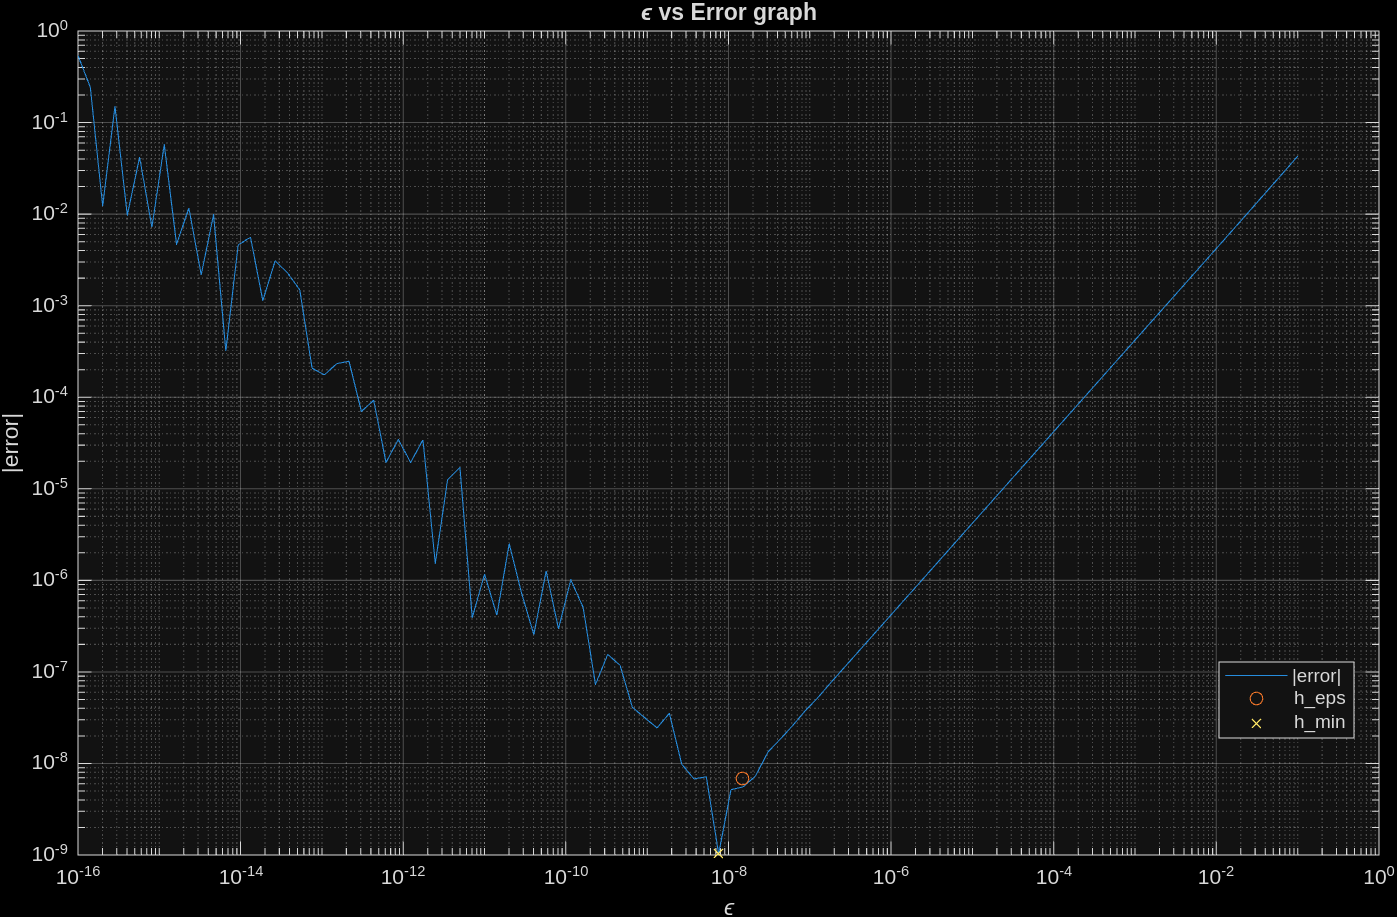
\includegraphics[width=0.5\linewidth]{question2/error_graph.png}
    \caption{Forward Difference Error vs $\epsilon$ Graph}
    \label{fig:forward_difference_error_vs_h}
\end{figure}

\section{Estimating the True Error Without an Analytical Solution}

Estimating errors in numerical ODE solving (Euler's Method) and the relation so step size. This can be done without knowing the exact analytical solution. We know that

\begin{equation}
    x_{t+1}^{(h)} = x_t + h f(x_t, t),
\end{equation}

and thus

\begin{equation}
    x_{t+1}^{(h/2)} = x_t + \frac{h}{2} f(x_t, t).
\end{equation}

If we define the exact solution of the ODE to be $y_t$, and assuming that the error in Euler's Method is $\mathcal{O}(h)$, we may write that

\begin{equation}
    y_t = x_t^{(h)} + Ch + \mathcal{O}(h^2).
\end{equation}

With the difference

\begin{equation}
    x_t^{(h/2)} - x_t^{(h)} = \bigg(y_t - C\frac{h}{2} - \mathcal{O}(h^2)\bigg) - \bigg(y_t - Ch - \mathcal{O}(h^2)\bigg)
\end{equation}

and ignoring the $\mathcal{O}(h^2)$ term,

\begin{equation}
    x_t^{(h)} - x_t^{(h/2)} = C \frac{h}{2}.
\end{equation}

Thus, we may estimate the error $Ch = y_t - x_t^{(h)}$ as

\begin{equation}
    \text{error}(h) \approx 2 \bigg(x_t^{(h)} - x_t^{(h/2)} \bigg)
\end{equation}

\begin{lstlisting}
% ===== Engineering Mathematics -- Homework 1 ===== %
% Author: Esraaj Sarkar Gupta
% Date: 1st February, 2026

% Housekeeping
clear; clc; close all;

% ---- Question 3 -- Euler: error vs step size ---- %
% ODE: dx(t) = p x(t),  x(0)=X0

p  = -1;     % Parameter
X0 =  4;     % Initial condition
T  =  5;     % Final time

% Step sizes
h_values = logspace(-4, -7, 100).';

% Exact value at T (solved analytically by esraaj)
xT_exact = X0 * exp(p*T);

% Arrays to store resultant data
err_true_T   = zeros(size(h_values));   % |x_h(T) - x_true(T)|

% Relative error esitmates
err_est_T    = zeros(size(h_values));   % |x_h(T) - x_h/2(T)|
err_est_2x   = zeros(size(h_values));   % 2*|x_h(T) - x_h/2(T)|

% --- Main loop-- sweep h --- %
for i = 1:numel(h_values)
    h = h_values(i);

    % Euler with step h
    [t_h, x_h] = Eulers_Method(X0, p, h, T);
    xT_h = x_h(end);

    [t_h2, x_h2] = Eulers_Method(X0, p, h/2, T);
    xT_h2 = x_h2(end);

    err_true_T(i) = abs(xT_h - xT_exact);

    err_est_T(i)  = abs(xT_h - xT_h2);

    err_est_2x(i) = 2 * err_est_T(i);
end

% ---- Plot: true error and the estimate ---- %
figure('Name','Euler: error vs h','NumberTitle','off');
loglog(h_values, err_true_T, 'LineWidth', 2); hold on;
loglog(h_values, err_est_T,  'LineWidth', 2);
loglog(h_values, err_est_2x, 'LineWidth', 2);
grid on
xlabel('h');
ylabel('Error at t = T');
title('Euler method: true error vs step-doubling estimate');
legend('|x_h(T) - x_{exact}(T)|', '|x_h(T) - x_{h/2}(T)|', '2|x_h(T) - x_{h/2}(T)|', ...
       'Location','best');
shg

% -- Local Functions -- %

function dX = f(X, p)
    dX = p * X;
end

function [t, X] = Eulers_Method(X0, p, h, T)
    % Euler method for scalar ODE X' = f(X,p), with X(0) = X0
    % We force the grid to land exactly on T.

    N = round(T/h) + 1;       % number of points
    t = linspace(0, T, N).';  % time vector
    h = t(2) - t(1);          % actual step used

    X = zeros(N,1);
    X(1) = X0;

    for k = 1:N-1
        X(k+1) = X(k) + h * f(X(k), p);
    end
end
\end{lstlisting}

\begin{figure}[!h]
    \centering
    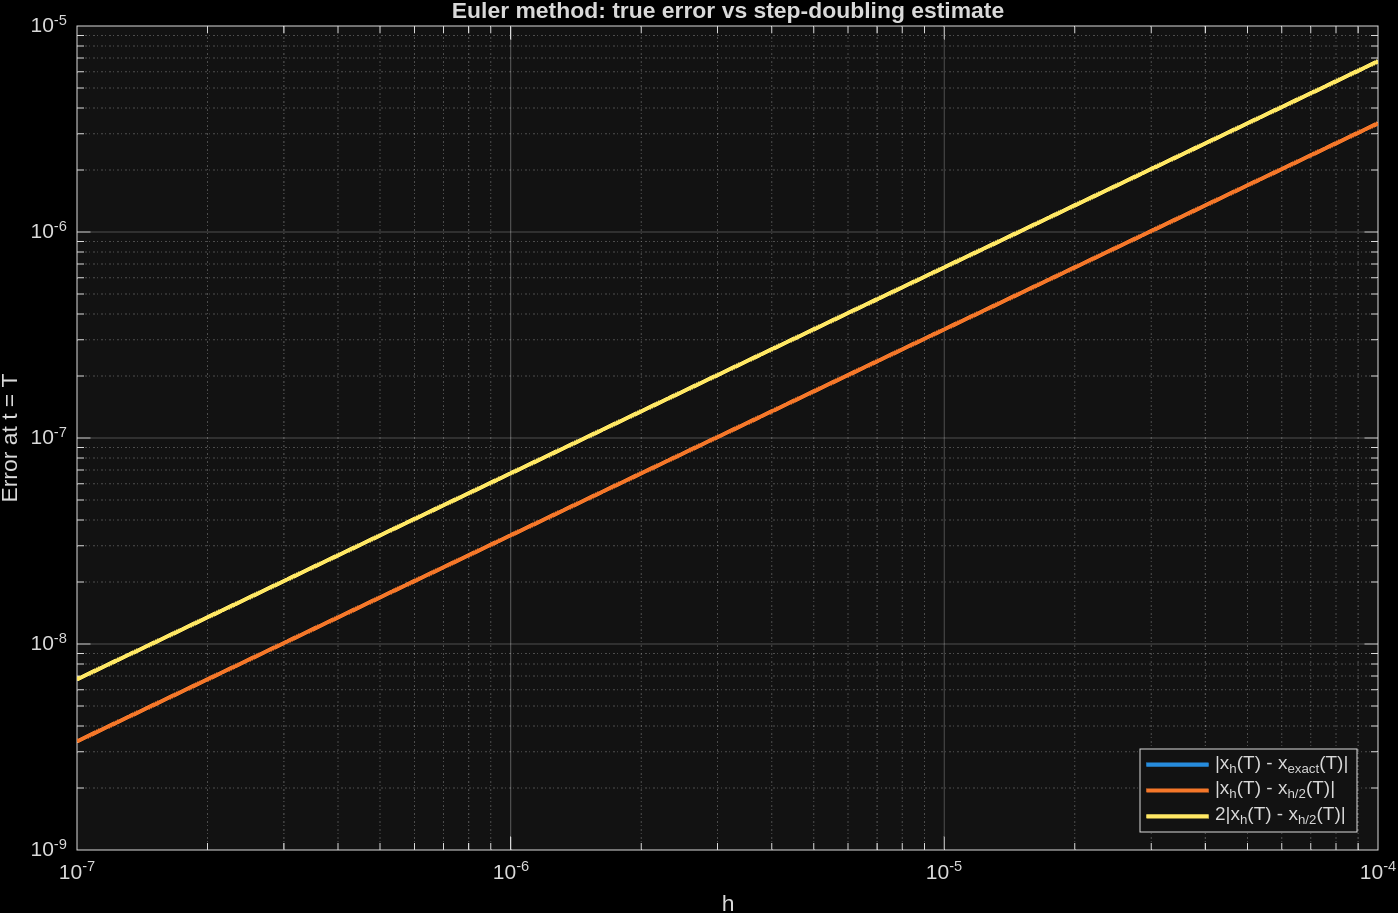
\includegraphics[width=0.5\linewidth]{question3/error_vs_h.png}
    \caption{Estimating the true error without an analytical solution}
    \label{fig:Estimating the true error without an analytical solution}
\end{figure}


\section{Solving ODEs using Euler's Method}

We find the solution to the ordinary differential equation $\dot{X} = pX$ for some arbitrary parameter $p \in \mathbb{R}$.\\
\\
The system $\dot{X} = -X$ is considered here. The step size $h$ and max time $T$ are passed to the solver as hyperparameters, along with the system's inital state \texttt{X0}.\\
\\
The number of iterations that the solver takes is calculated as
$N = \texttt{round}(T/h)$. 

\begin{lstlisting}
% ===== Engineering Mathematics -- Homework 1 ===== %
% Author: Esraaj Sarkar Gupta
% Date: 1st February, 2026

% ---- Question 4 -- Euler's Method ---- %

p = [-1];   % Parameter list
X0 = [4];   % Initial Conditions: x_0,
h = 0.01;   % Step size
T = 5;      % Final time

% Main Function
[t, X] = Eulers_Method(X0, p, h, T);

% Plotting
plot(t, X)
xlabel('t'); ylabel('X(t)')
title('Euler method solution')
grid on
shg

% -- Local Functions -- %

function dX = f(X, p)
    dX = p * X;
end

function [t, X] = Eulers_Method(X0, p, h, T)
    N = round(T/h) + 1;         % Number of steps
    t = linspace(0, T, N).';    % Time values
    X = zeros(N,1);             % X values
    X(1) = X0;                  % Initial X value
    
    % Main loop
    for k = 1:N-1
        X(k+1) = X(k) + h * f(X(k), p);
    end
end
\end{lstlisting}

\begin{figure}
    \centering
    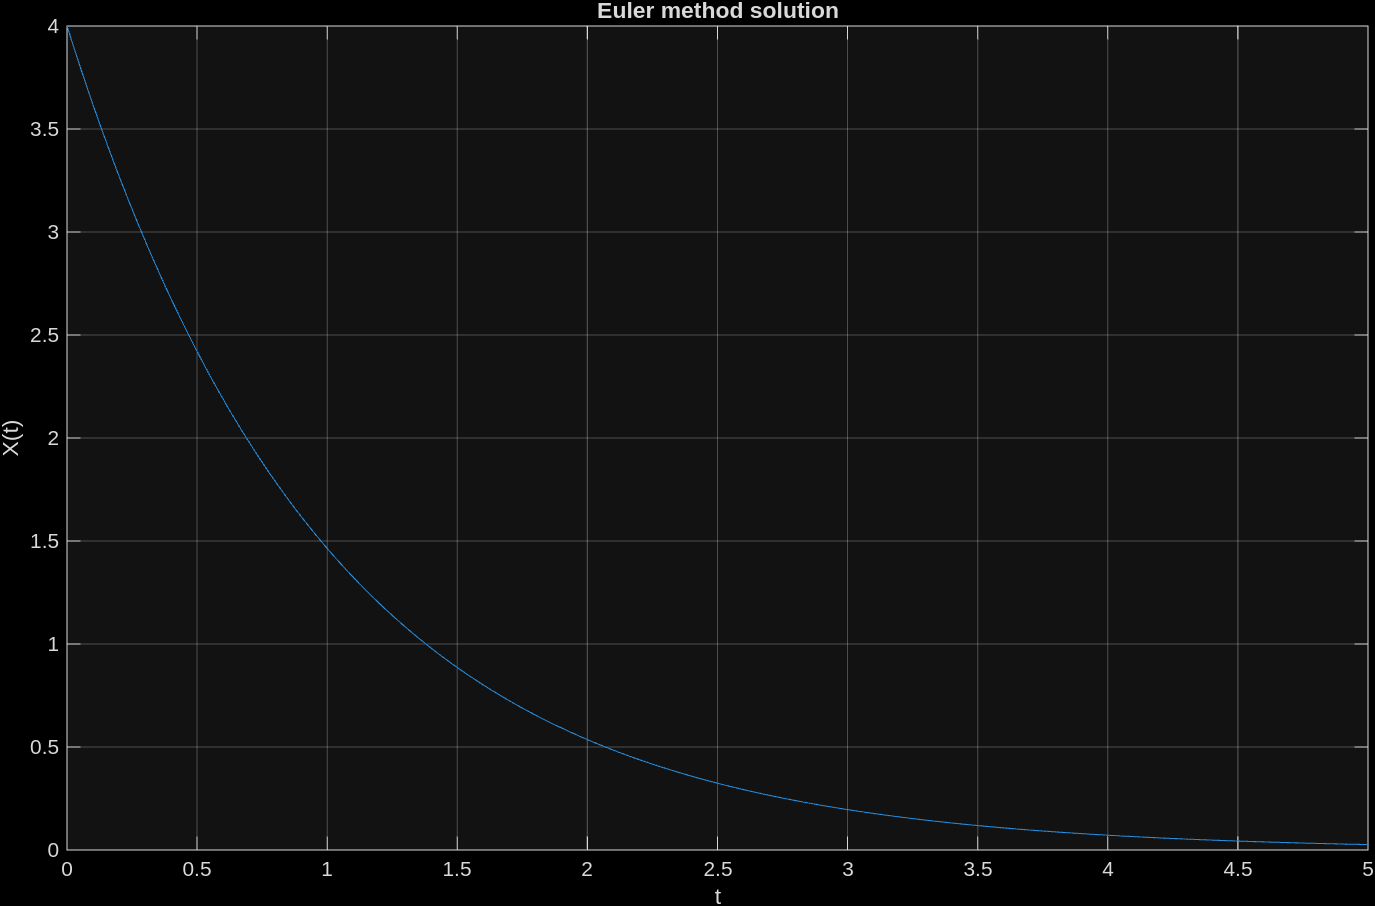
\includegraphics[width=0.5\linewidth]{question4/euler_solution.png}
    \caption{Euler Method Solution to $\dot{X} = pX$}
    \label{fig:placeholder}
\end{figure}

\section{The Motion of a Double Pendulum}

The system consists of a double pendulum modeled with two point masses ($m_1, m_2$) and two linkages ($R, \delta$). This setup represents a coupled, non-linear dynamical system where the motion of the secondary mass is governed by both gravitational potential and the inertial torque transmitted through the primary linkage, leading to characteristic chaotic behavior.\\
\\
The dynamics were derived via Lagrangian Mechanics. To simplify the implementation, the system is expressed using the following geometric and inertial constants:

\begin{align*}
    A &= \frac{1}{3}m_1 R^2 + 1.5 m_2 \delta^2 \\
    B &= 1.5 \delta^2 \\
    C &= 2 m_2 g R \\
    D &= m_2 B \\
    E &= 2 m_2 g \delta
\end{align*}

The second-order coupled ordinary differential equations (ODEs) for the angular displacements $\theta$ and $\phi$ are given by:

\begin{equation}
    \ddot{\theta} = \frac{B E \cos(\phi) - C D \sin(\theta)}{AD}
\end{equation}

\begin{equation}
    \ddot{\phi} = \frac{-(A+B) E \cos(\phi) + C D \sin(\theta)}{AD}
\end{equation}

For numerical integration, these are reduced to a first-order system $\dot{\mathbf{y}} = f(t, \mathbf{y})$ where $\mathbf{y} = [\theta, \dot{\theta}, \phi, \dot{\phi}]^T$.

\begin{lstlisting}
% ===== Engineering Mathematics -- Homework 1 ===== %
% Author: Esraaj Sarkar Gupta
% Date: 1st February, 2026

% Housekeeping
clear; clc; close all;

% ---- Question 5 -- Equations of Motion of a Double Pendulum ---- %

% -- System Parameters -- %
g = 9.8;
m1 = 2;
m2 = 3;
R = 10;
delta = 3;

% Simplify parameteras (for the sake of our sanity)
A = (m1 * R^2 / 3) + (1.5 * m2 * delta^2);
B = 1.5 * delta^2;
C = 2 * m2 * g * R;
D = m2 * B;
E = 2 * m2 * g * delta;

% Parameter Vector
p = [A; B; C; D; E];

% -- Time Spans -- %
t0 = 0;
T  = 20;

% Euler step size
h = 1e-6;

% -- Intial Conditions -- %
y0 = [1.0; 0.0; 0.0; 0.0]; % y = [theta, theta_dot, phi, phi_dot]

% -- Main Function --%
rhs = @(t,y) coupled_system_rhs(t, y, p);

% Solve using Euler
[t, Y] = euler_system(rhs, t0, T, y0, h);

theta     = Y(:,1);
theta_dot = Y(:,2);
phi       = Y(:,3);
phi_dot   = Y(:,4);

% ---- Plotting ---- %
figure('Name','Angles vs time','NumberTitle','off');
plot(t, theta, 'LineWidth', 2); hold on;
plot(t, phi,   'LineWidth', 2);
xlabel('Time');
ylabel('Angle (radians)');
legend('\theta_1(t)','\theta_2(t)','Location','best');
grid on;
title('Euler Method Solution of the Coupled System');
shg

figure('Name','Phase space','NumberTitle','off');

subplot(1,2,1);
plot(theta, theta_dot, 'LineWidth', 1.5);
xlabel('\theta_1'); ylabel('\dot{\theta_1}');
title('Phase Space: \theta_1 vs. \dot{\theta_1}');
grid on;

subplot(1,2,2);
plot(phi, phi_dot, 'LineWidth', 1.5);
xlabel('\theta_2'); ylabel('\dot{\theta_2}');
title('Phase Space: \theta_2 vs. \dot{\theta_2}');
grid on;

shg

%{
    One may observe non-linear patterns and chaotic aperiodicity in these
    graphs, indicative of a double pendulum's chaotic motion. This is
    especially evident in the non-closed phase diagrams.
%}

% == Local Functions == %
%{
    Likely to Professor Ruina's disappointment, I derived these equations
    of motion of a double pendulum using Lagrangian Mechanics as opposed to
    having used moment balance.

    One day I will learn to do better.
%}

function dydt = coupled_system_rhs(~, y, p)
    % Unpack parameters
    A = p(1); B = p(2); C = p(3); D = p(4); E = p(5);

    % y = [theta, theta_dot, phi, phi_dot]
    theta     = y(1);
    theta_dot = y(2);
    phi       = y(3);
    phi_dot   = y(4);

    % Equations of Motion
    theta_ddot = (B * E * cos(phi) - C * D * sin(theta)) / (A * D);
    phi_ddot   = (-A * E * cos(phi) - B * E * cos(phi) + C * D * sin(theta)) / (A * D);

    dydt = [theta_dot; theta_ddot; phi_dot; phi_ddot];
end

function [t, Y] = euler_system(rhs, t0, tf, y0, h)
    % Euler integrator for vector ODEs y' = rhs(t,y)
    arguments
        rhs (1,1) function_handle
        t0  (1,1) double
        tf  (1,1) double
        y0  (:,1) double
        h   (1,1) double {mustBePositive}
    end

    N = floor((tf - t0)/h) + 1;
    t = t0 + (0:N-1)'*h;

    nstate = numel(y0);
    Y = zeros(N, nstate);
    Y(1,:) = y0.';

    for k = 1:N-1
        yk = Y(k,:).';
        Y(k+1,:) = (yk + h * rhs(t(k), yk)).';
        % If you start seeing NaNs, your step is too big (Euler is fragile).
    end
end
\end{lstlisting}

\begin{figure}[!h]
    \centering
    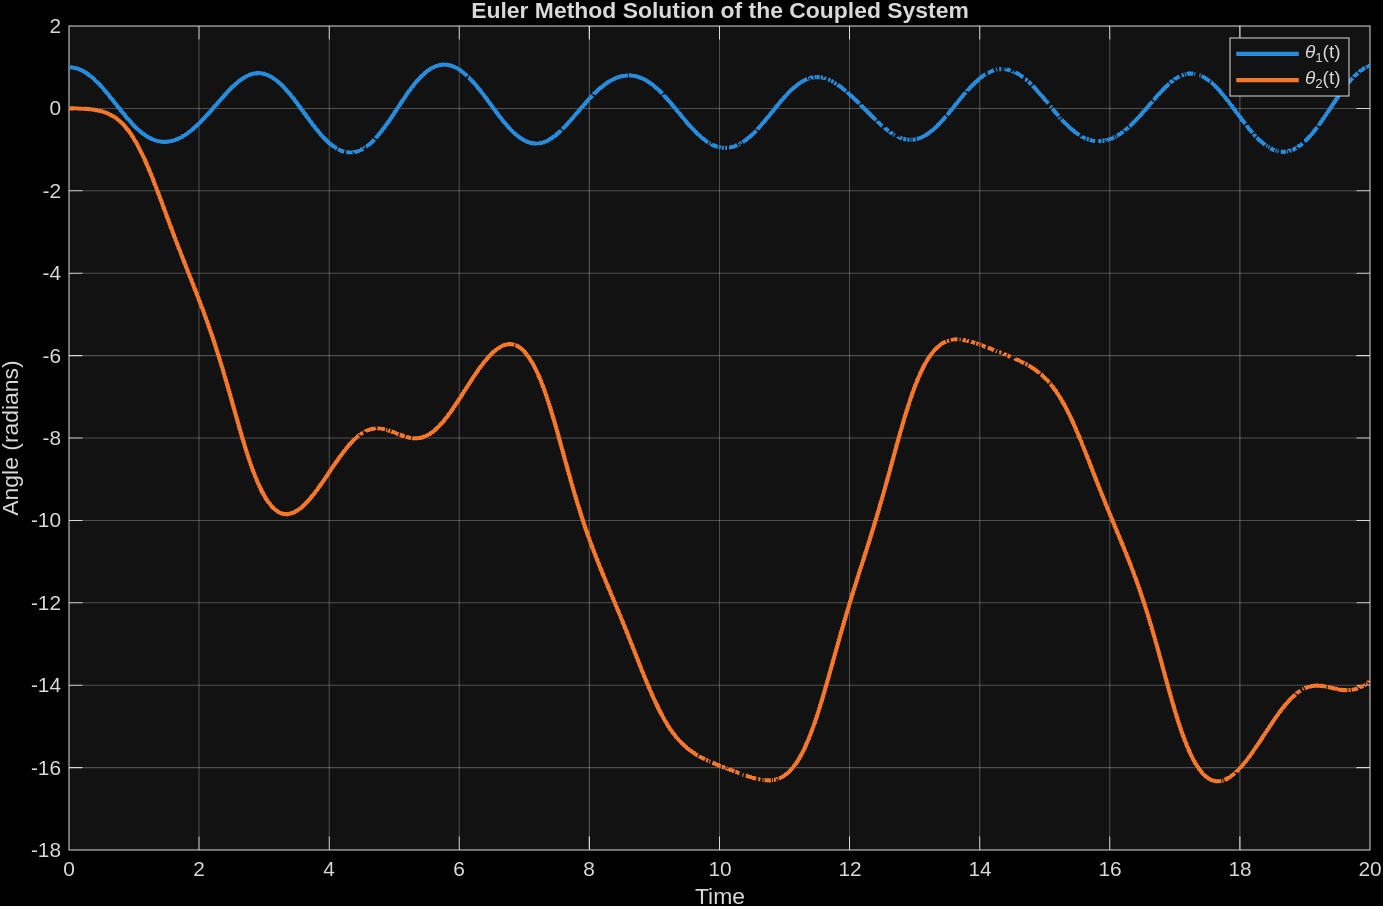
\includegraphics[width=0.5\linewidth]{question5/dPendu_angles_vs_time.png}
    \caption{Double Pendulum Angles vs Time}
    \label{fig:placeholder}
\end{figure}

The simulation yields several key insights into the nature of coupled oscillations:
\begin{itemize}
    \item \textbf{Chaotic Aperiodicity:} The time-series plot of $\theta_1(t)$ and $\theta_2(t)$ demonstrates a lack of repeating patterns. Unlike a simple pendulum, the energy transfer between the two masses prevents a simple harmonic steady state.
    \item \textbf{Phase Space Divergence:} The phase diagrams ($\theta_1$ vs. $\dot{\theta_1}$ and $\theta_2$ vs. $\dot{\theta_2}$) show non-closed trajectories. In a dissipative or simple periodic system, these would form closed loops or spirals; here, they fill the phase plane in a manner indicative of strange attractors.
    \item \textbf{Numerical Sensitivity:} The "Euler fragility" mentioned in the source code is evident. Because Euler's method does not conserve energy, small errors in the $\ddot{\theta_1}$ calculation accumulate rapidly, necessitating the infinitesimal step size to prevent the solution from diverging to infinity (NaN results).
\end{itemize}

\begin{figure}[h!]
    \centering
    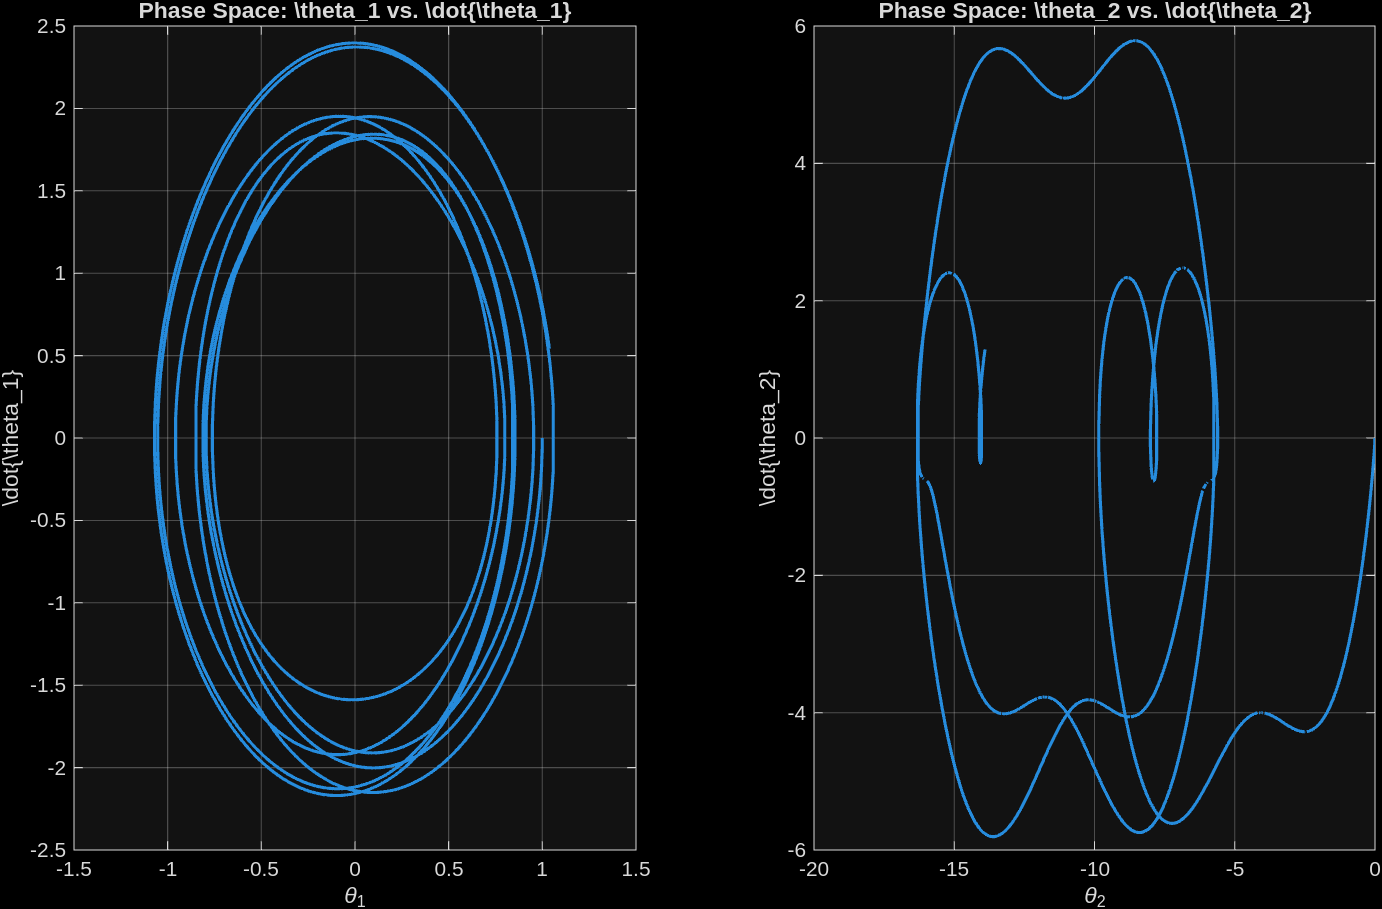
\includegraphics[width=0.8\linewidth]{question5/dPendu_phase_space.png}
    \caption{Double Pendulum Phase Spaces}
    \label{fig:placeholder}
\end{figure}


\section{Central Difference Differentiation -- RK2}

This analysis explores the numerical approximation of the derivative of $f(x) = \sin(x)$. By comparing the Forward Difference and Central Difference methods across a logarithmic range of step sizes ($10^{-2}$ to $10^{-16}$), we characterize the transition from discretization-limited regimes to precision-limited regimes.\\
\\
The Central Difference method is a second-order approximation derived from the Taylor series expansion. The formula used for evaluation is:

\begin{equation}
    f'(x) \approx \frac{f(x + h) - f(x - h)}{2h}
\end{equation}

For comparison, the first-order Forward Difference method is defined as:

\begin{equation}
    f'(x) \approx \frac{f(x + h) - f(x)}{h}
\end{equation}

\begin{lstlisting}
% ===== Engineering Mathematics -- Homework 2, Question 6 ===== %
% Author: Esraaj Sarkar Gupta
% Date: 8th February, 2026

% Housekeeping
clc; clear; close all;

% ==== Higher Order Methods ==== %

%% Part A -- Differentiation using Central Difference %%


% -- Function to be Differentiated -- %
f = @(x) sin(x);

% True analytic derivative
df = @(x) cos(x);

% ---- Numerical Evaluation -- Central Difference Method ---- %

% delta_f(x) ~ f(x + h) - f(x-h) / 2h


X0  = 1.0;

% -- List of h values -- %
h_values = logspace(-2, -16, 100);
evaluation = central_difference(f, X0, h_values);

% ---- Error Evaluation ---- %
true_val = df(X0);
errors = abs(true_val * ones(size(h_values)) - evaluation);

% Plot
figure;
loglog(h_values, errors, 'o-', 'LineWidth', 1.6, 'MarkerSize', 4);
xlabel('h', 'FontSize', 12)
ylabel('Absolute error', 'FontSize', 12)
title('Central difference error for d/dx(sin x) at x=0', 'FontSize', 13)
legend('Central difference', 'Location', 'best')
set(gca, 'FontSize', 11, 'LineWidth', 1.1)
hold off
shg;

% ---- Comparing h error vs Forward Difference Method ---- %
evaluation_forward_difference = forward_difference(f, X0, h_values);
errors_forward_difference = abs(true_val * ones(size(h_values)) - evaluation_forward_difference);

% Comparision plot
figure;
loglog(h_values, errors, 'o-', 'LineWidth', 1.6, 'MarkerSize', 4);
hold on
loglog(h_values, errors_forward_difference, 's--', 'LineWidth', 1.6, 'MarkerSize', 4);
hold off
xlabel('h', 'FontSize', 12)
ylabel('Absolute error', 'FontSize', 12)
title('Comparison between central difference and forward difference methods for sin(x = 0).', 'FontSize', 13)
legend('Central difference', 'Forward difference', 'Location', 'best')
set(gca, 'FontSize', 11, 'LineWidth', 1.1)
shg;


% ---- Functions ----- #
function delta_f = central_difference(f, x, h)
    delta_f = ( f(x + h) - f(x - h)) ./ (2*h);
end

function delta_f = forward_difference(f, x, h)
    delta_f = ( f(x + h) - f(x) ) ./ h;
end

%% Part B -- Solving ODEs using the Midpoint Method %%

% Housekeeping
clear;

% -- System -- %
p = [1];     % Parameters
X0 = [4];    % Intial conditions
h = 1e-4;    % Step size
T = 5;       % Final time

% -- Main Function -- %
[t, X] =  RK2(X0, p, h, T);

% Plotting
figure;
plot(t, X)
xlabel('t'); ylabel('X(t)')
title('RK2 (Midpoint Method) solution')
grid on
shg

% -- Local Functions -- %
function dX = g(X, t, p)
arguments
    X
    t
    p (1,1) double = 1
end
    % Example: time-dependent system dX/dt = p * t * X
    % (uses t explicitly; p is correctly applied as a scalar parameter)
    dX = p * t .* X;
end


function [t, X] = RK2(X0, p, h, T)
    N = round(T/(2*h)) + 1;     % Number of steps
    t = linspace(0, T, N).';    % Time values
    X = zeros(N, 1);            % Init X values
    X(1) = X0;                  % Initial value

    for k = 1:N-1
        X_mid = X(k) + g(X(k), t(k), p) * (h/2);
        X(k+1) =  X(k) + h * g(X_mid, t(k) + h/2);
    end
end
\end{lstlisting}


\begin{figure}
    \centering
    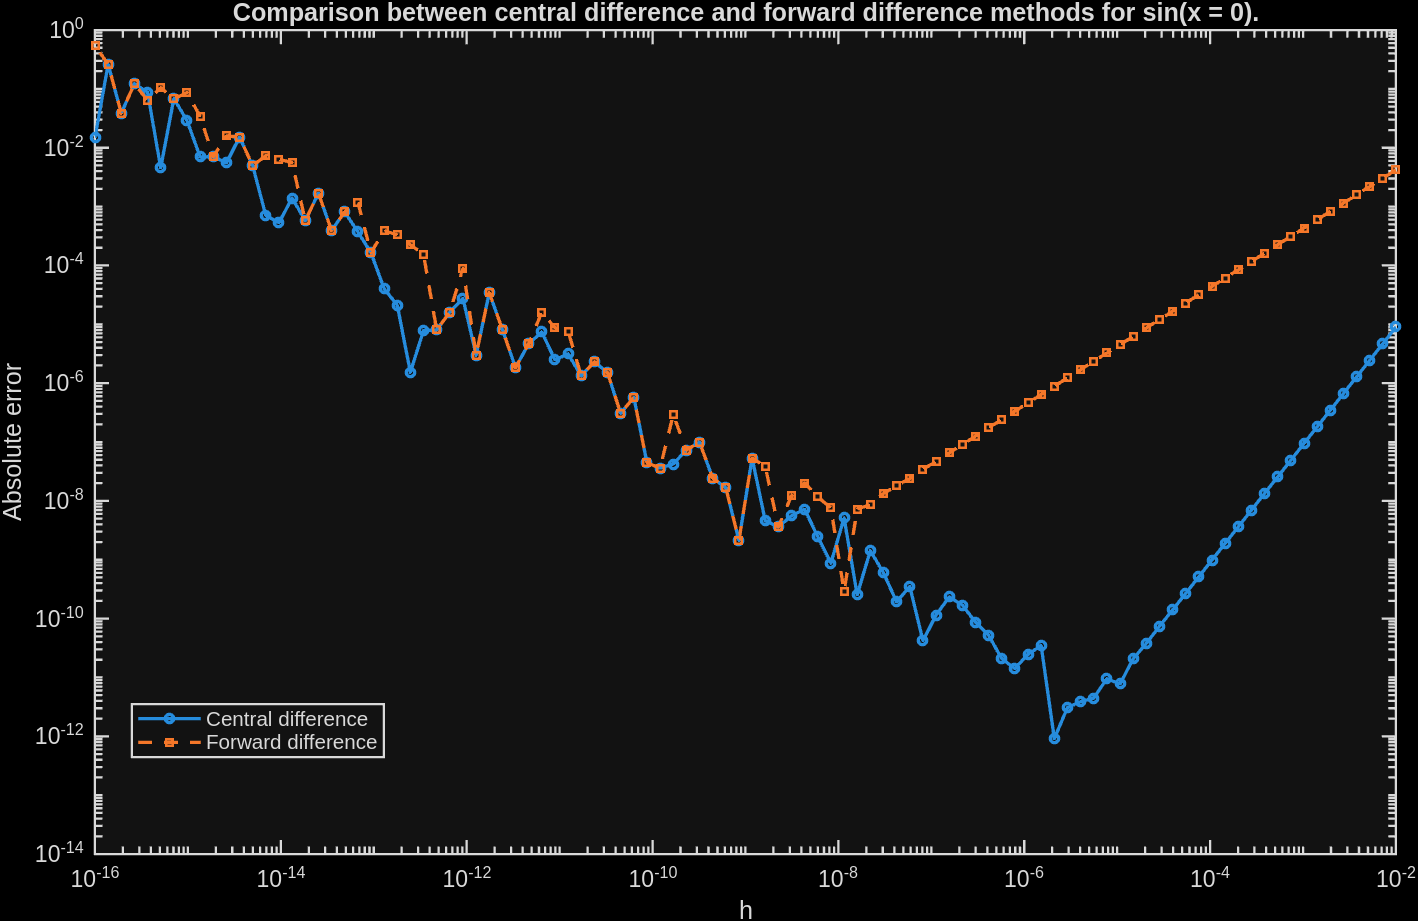
\includegraphics[width=0.5\linewidth]{question6/rk2_vs_euler_error.png}
    \caption{Forward Difference Differentiation vs Central Difference Differentiation}
    \label{fig:placeholder}
\end{figure}

The log-log error plot (Fig. 1) reveals the fundamental constraints of numerical computing:

\begin{itemize}
    \item \textbf{Order of Accuracy (Slopes):} In the right-hand side of the graph ($h > 10^{-8}$), the error decreases as $h$ gets smaller. The Central Difference curve has a steeper slope of 2 in the log-log space, confirming its $O(h^2)$ truncation error, while the Forward Difference curve follows a slope of 1, confirming $O(h)$.

        \begin{eqnarray}
        E & = & Ch^2 \nonumber \\
        \log(E) & = & \log(C) + 2\log(h)
        \end{eqnarray}
    
    \item \textbf{The "V-Shape" (Round-off Error):} Below a critical $h$ value, the error stops decreasing and begins to increase. This is due to \textit{floating-point subtraction error}. As $h \to 0$, the values of $f(x+h)$ and $f(x-h)$ become so similar that their subtraction results in a loss of significant digits, amplified by the $1/h$ term in the denominator.
    
    \item \textbf{Optimal Step Size:} The Central Difference method achieves a significantly lower minimum error ($\approx 10^{-12}$) compared to the Forward Difference ($\approx 10^{-8}$). Furthermore, the "sweet spot" for Central Difference occurs at a larger $h$ ($\approx 10^{-5.5}$) than the Forward Difference ($\approx 10^{-8}$), making it both more accurate and computationally more robust against round-off.

\end{itemize}

\subsection{A Challenge : Estimating the slope of the floating-point errors}

It is fairly obvious that the slope of errors in the central difference method is twice of the forward difference method. Expanding $f(x+h)$ in its Taylor Series, 
\begin{equation}
    f(x+h) = f(x) + h\frac{df(x)}{dx} + \frac{h^2}{2}\frac{d^2f(x)}{dx^2} + \dots
\end{equation}

Ignoring the second order terms, we get 

\begin{equation}
    \frac{df(x)}{dx} = \frac{f(x+h) - f(x)}{h}
\end{equation}

which in the log-log space, is

\begin{equation}
    \log(\text{error}) = \log(f(x+h) - f(x)) = 1 \cdot \log(h) + \log(C_1)
\end{equation}

in the form of a straight line $y = mx + c$.

In central difference, $f(x+h) - f(x-h)$ is approximated to

\begin{equation}
    \frac{f(x+h) - f(x-h)}{2h} = \frac{df}{dx} + \frac{h^2}{6}\frac{d^3f}{dx^3} + \dots
\end{equation}

which gives us a log-log expression of 

\begin{equation}
    \log(\text{error}) = 2 \log\bigg(\frac{h}{6}\bigg) + \log(C_2).
\end{equation}

The accuracy of a 16-bit computer is bound by \textit{machine epsilon} $\epsilon_m \approx 10^{-16}$. As $h$ is decreased to the same order of $\epsilon_m$, we see that $f(x) \approx f(x+h) \approx f(x-h)$. Subtracting nearly identical numbers on a computer results in a phenomenon known as \textit{catastrophic subtraction}, where only the roundoff noise remains and is stored as the result of the computation.\\
\\
Here the roundoff error is given by the following expression since in both cases, the result of the catastrophic subtraction is divided by $h$.
\begin{equation}
    E_\text{rf} \approx \frac{\epsilon_m}{h}
\end{equation}

In the log-log space, this expression clearly demonstrates a slope of $-1$ as $h$ varies irrespective of the coefficient of $h$.

\begin{equation}
    \log(E_\text{rf}) = -1 \log(hc) + \log(\epsilon_m) = -1 \log(h) + \log(C_3).
\end{equation}

This derived result is consistent with observation.

\section{Spring and Mass System}

% Definition of the radial distance and unit vector
Let $r = \sqrt{x^2 + y^2}$ be the magnitude of the position vector, and $\hat{e} = \frac{x\mathbf{i} + y\mathbf{j}}{r}$ be the unit vector in the radial direction.

% The coupled differential equations
\begin{align}
    \ddot{x} &= -\frac{k}{m} \left( r - L_0 \right) \frac{x}{r} \label{eqn:question7_eomx}\\
    \ddot{y} &= -g - \frac{k}{m} \left( r - L_0 \right) \frac{y}{r} \label{eqn:question7_eomy}
\end{align}

\begin{lstlisting}
% ===== Engineering Mathematics -- Homework 2, Question 7 ===== %
% Author: Esraaj Sarkar Gupta
% Date: 8th February, 2026

% Housekeeping
clc; clear; close all;

%% Part A -- Equations of Motion %%

%{
    Equations of Motion (derived analytically)

    x_ddot = (1/m) [ -k ( sqrt(x^2 + y^2) - L0) \hat{e} dot i]
    y_ddot = (1/m) [(-mg) - k ( sqrt(x^2 + y^2) - L0 \hat{e} dot j]
    
        where \hat{e} = (xi + yj) / sqrt(x^2 + y^2)
%}

%% Part B -- Plotting the Trajectory of the Mass

% System parameter struct
params.m  = 1.0;
params.k  = 1000.0;
params.L0 = 5.0;
params.g  = 9.81;

S0 = [5.0; 0.0; 0.0; 0.0];          % [x0; y0; vx0; vy0]
tspan = [0 10];                      % Initial time, Final time

h = 1e-3;

% -- SOLVE -- %
[t, S] = RK2(@(t,S) system(t,S,params), tspan, S0, h);

% -- Plotting Results -- %

x = S(:,1);
y = S(:,2);

figure;
plot(x, y, 'LineWidth', 1.5);
axis equal
grid on
xlabel('x'); ylabel('y');
title('Trajectory of the mass (RK2 Midpoint)');

% -- Animation -- %
fig = figure;
ax = axes(fig);
cla(ax, 'reset');
hold(ax, 'on');
axis(ax, 'equal');
grid(ax, 'on');
xlabel(ax, 'x'); ylabel(ax, 'y');
title(ax, 'Animation of System');

% -- Lock Figure Axes -- %
pad = 0.1;  % 10% padding
xmin = min(x); xmax = max(x);
ymin = min(y); ymax = max(y);

xr = xmax - xmin;  yr = ymax - ymin;

if xr == 0, xr = 10; end
if yr == 0, yr = 10; end

xlim(ax, [xmin - pad*xr, xmax + pad*xr]);
ylim(ax, [ymin - pad*yr, ymax + pad*yr]);

axis(ax, 'manual');

% Create handles
mass_pt   = plot(ax, x(1), y(1), 'o', 'MarkerSize', 10, 'LineWidth', 2);
spring_ln = plot(ax, [0 x(1)], [0 y(1)], '-', 'LineWidth', 1.5);
trail_ln  = plot(ax, x(1), y(1), '-', 'LineWidth', 1.2);

trail_len = 300;
skip = 5;

for k = 1:skip:length(t)
    % -- Dynamically update plot elements -- %
    set(mass_pt,   'XData', x(k),     'YData', y(k));
    set(spring_ln, 'XData', [0 x(k)], 'YData', [0 y(k)]);

    k0 = max(1, k - trail_len);
    set(trail_ln,  'XData', x(k0:k),  'YData', y(k0:k));

    drawnow;
end


% -- Local Functions -- %

% Modelling the System
function dS = system(t, S, params)

% -- Unpack State -- %
% Python tuple unpacking is better <\3
x  = S(1);
y  = S(2);
vx = S(3);
vy = S(4);

% -- Unpack parameter structure -- % 
m  = params.m;
k  = params.k;
L0 = params.L0;
g  = params.g;

% -- Geometry -- %
r2 = x^2 + y^2;
r  = sqrt(r2);
if r == 0
    e_x = 0;
    e_y = 0;
else
    e_x = x / r;
    e_y = y / r;
end

deltaL = r - L0;

% -- Forces -- %

F_spring_mag = -k * deltaL;
F_spring_x   = F_spring_mag * e_x;
F_spring_y   = F_spring_mag * e_y;

F_grav_x = 0;
F_grav_y = -m * g;

F_net_x = F_spring_x + F_grav_x;
F_net_y = F_spring_y + F_grav_y;

ax = F_net_x / m;
ay = F_net_y / m;

% -- Pack Derivatives -- %

dx  = vx;
dy  = vy;
dvx = ax;
dvy = ay;


dS = [dx; dy; dvx; dvy];
end

function [t, S] = RK2(f, tspan, S0, h)
    t0 = tspan(1);
    tf = tspan(2);

    N = floor((tf - t0)/h) + 1;      % Number of steps
    t = (t0 + (0:N-1)*h).';          % Time values

    S = zeros(N, numel(S0));         % State history
    S(1,:) = S0(:).';                % Initial state

    for k = 1:N-1
        tk = t(k);
        Sk = S(k,:).';               % column state

        k1 = f(tk, Sk);
        S_mid = Sk + (h/2)*k1;

        k2 = f(tk + h/2, S_mid);
        S_next = Sk + h*k2;

        S(k+1,:) = S_next.';
    end
end

%}

\end{lstlisting}


\begin{itemize}
\item \textbf{No Spring (k=0):} In the absence of spring force, the mass behaves as a projectile. It falls vertically if the initial velocity is zero and follows a parabolic trajectory if the initial velocity is non-zero.
\item \textbf{Rigid Connection ($k\approx 10^5$ ):} Theoretically, an infinitely stiff spring should mimic a rigid pendulum. With the right initial conditions ($\Delta L = 0, \vec{v}_0 = 0$), this result is observed in the numerical solution.
\item \textbf{Zero Gravity and Velocity (g=0,v=0):} Under these conditions, the system's motion is constrained to a straight line, as there are no external lateral forces to perturb the radial oscillation of the spring.
\item \textbf{Zero Rest Length $(L_0 = 0)$:} When the rest length is zero, the spring force becomes perfectly linear along both the x and y axes. This simplifies the system into a 2D harmonic oscillator, causing the mass to move along a radial line passing through the origin.
\end{itemize}

\begin{figure}[htbp]
     \centering
     % --- Row 1 ---
     \begin{subfigure}[b]{0.45\textwidth}
         \centering
         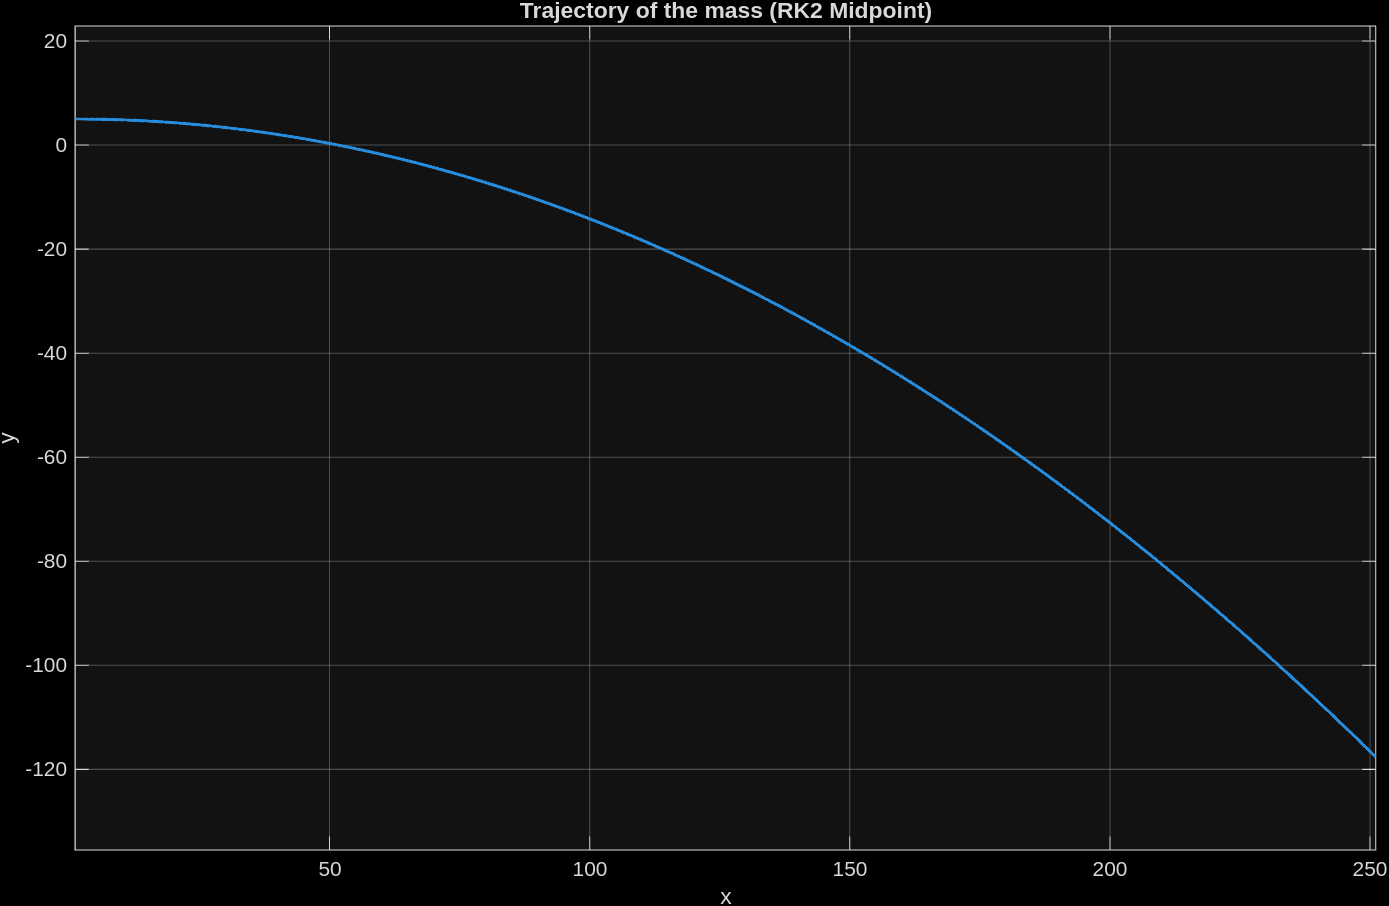
\includegraphics[width=\textwidth]{question7/kzero.png}
         \caption{No Spring ($k=0$)}
         \label{fig:k0}
     \end{subfigure}
     \hfill
     \begin{subfigure}[b]{0.45\textwidth}
         \centering
         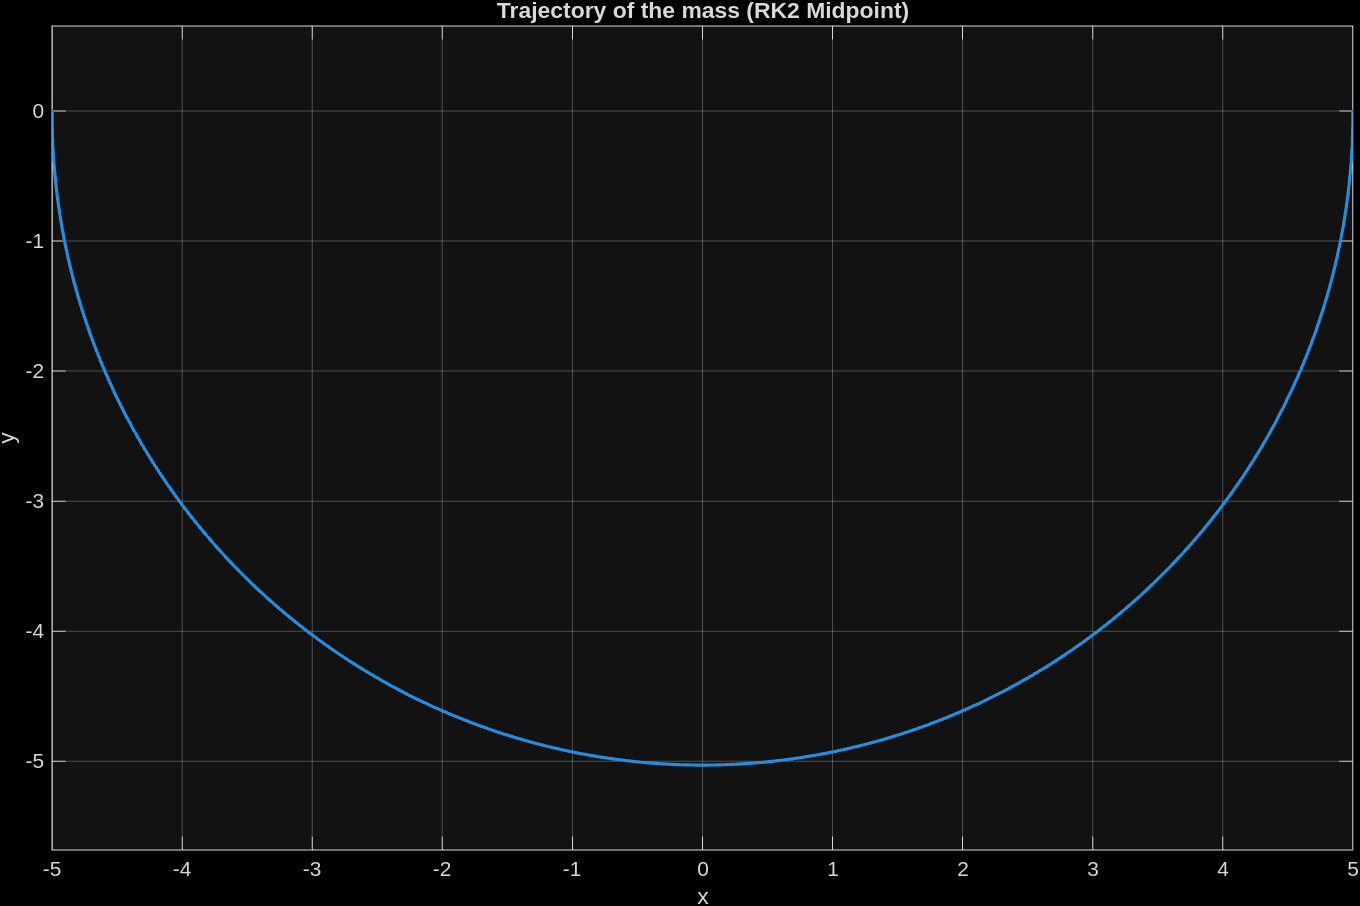
\includegraphics[width=\textwidth]{question7/pendu.png}
         \caption{Rigid Connection}
         \label{fig:rigid}
     \end{subfigure}

     \vspace{0.5cm} % Add some vertical spacing between rows

     % --- Row 2 ---
     \begin{subfigure}[b]{0.45\textwidth}
         \centering
         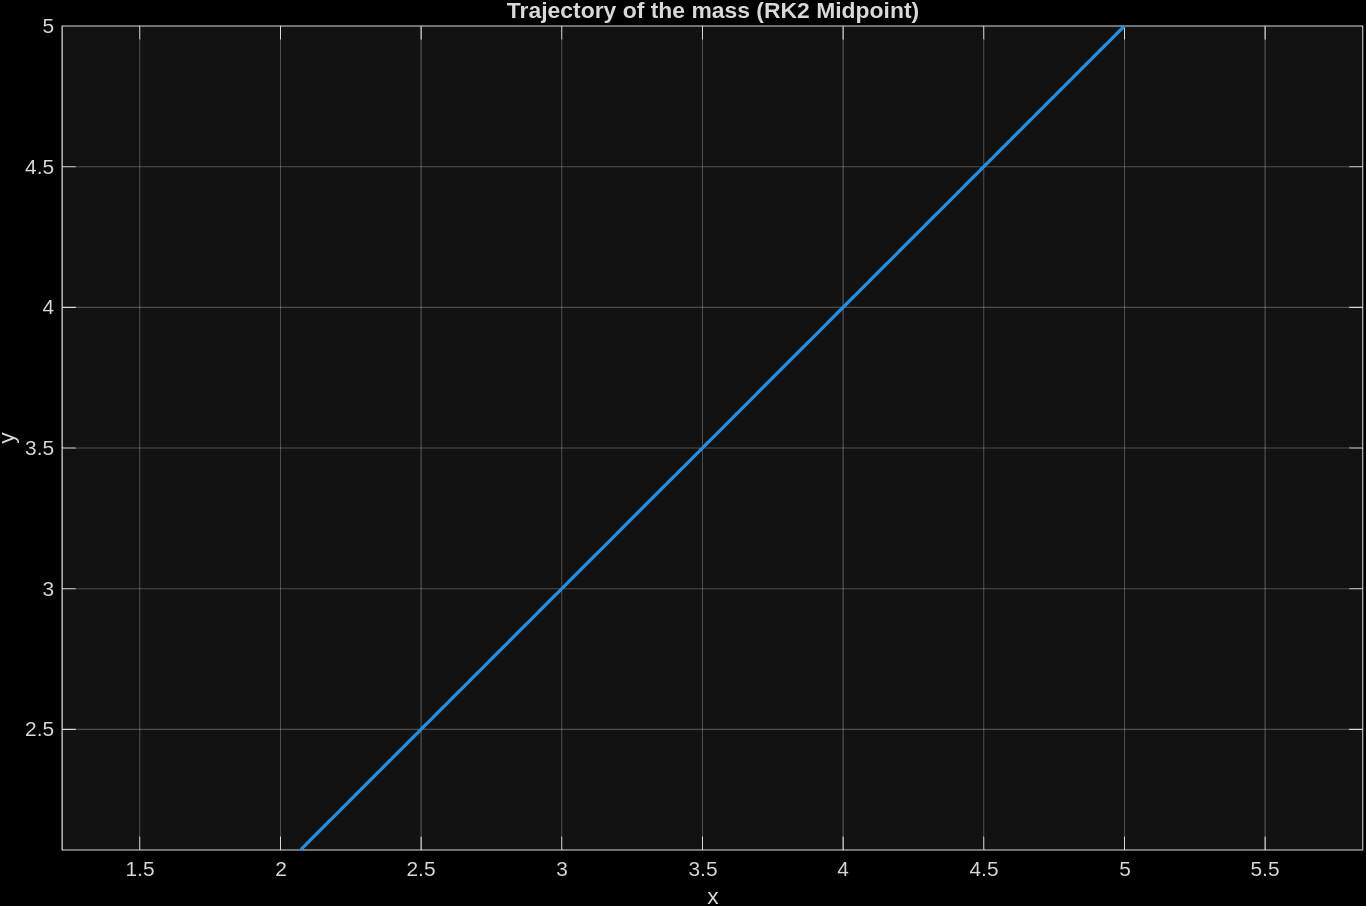
\includegraphics[width=\textwidth]{question7/gzero_vzero.png}
         \caption{Zero Gravity ($g=0$)}
         \label{fig:g0}
     \end{subfigure}
     \hfill
     \begin{subfigure}[b]{0.45\textwidth}
         \centering
         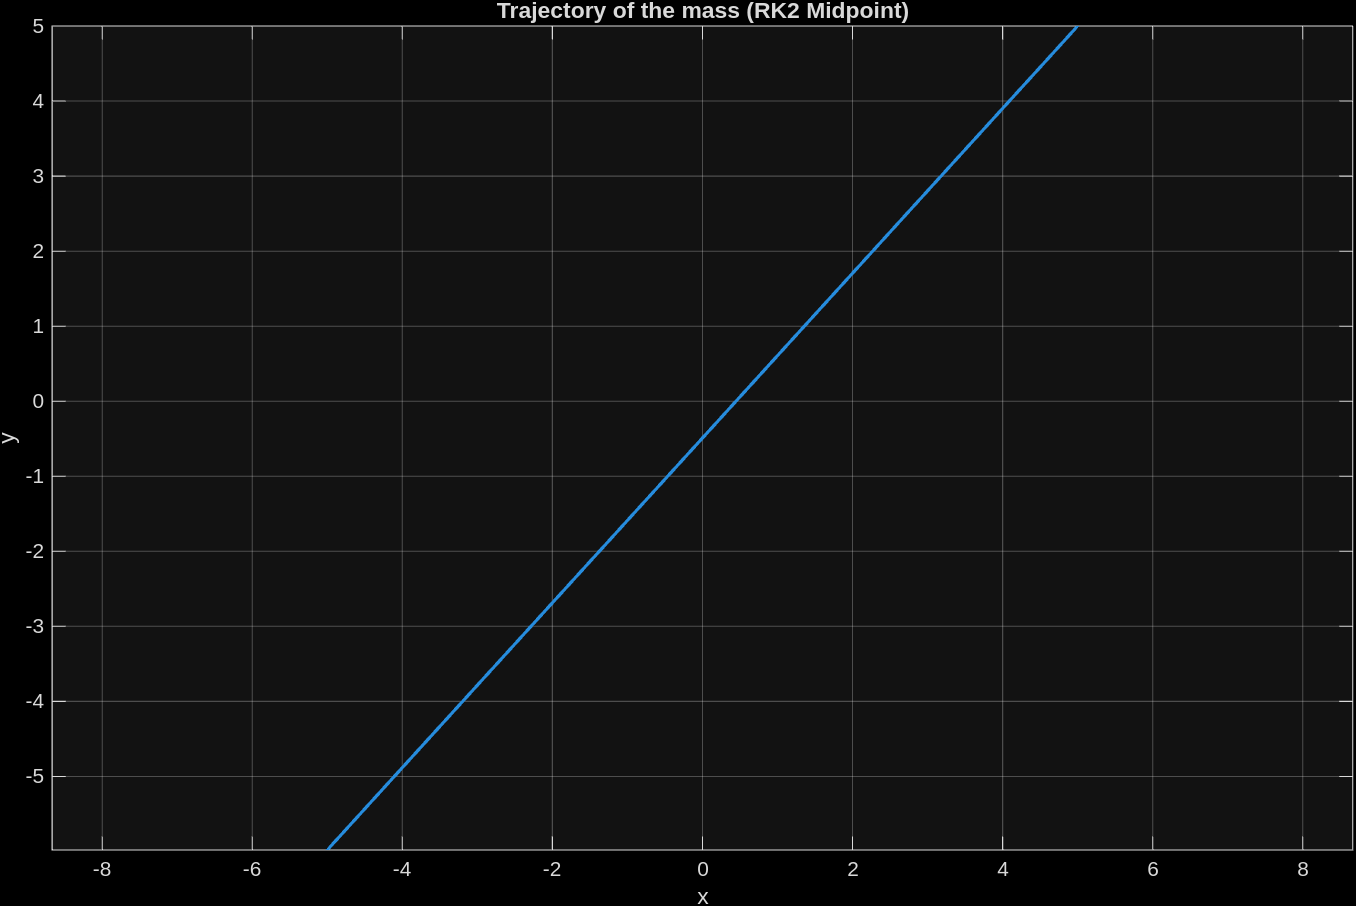
\includegraphics[width=\textwidth]{question7/harmonic_oscillator.png}
         \caption{Zero Rest Length ($L_0=0$), Harmonic Oscillator}
         \label{fig:L0}
     \end{subfigure}
     
     \caption{Numerical Simulation Results for Various System Parameters}
     \label{fig:results_grid}
\end{figure}

\subsection{A Challenge: Circular Motion in the Harmonic Oscillator}
In this subsection we attempt to derive the system parameters required to simulate circular motion in the \textbf{Zero Rest Length} case where the system behaves like a 2D harmonic oscillator.\\

Any 2D system in circular motion may be described with the positions

\begin{align}
    x &= A\cos(\omega t) \\
    y &= A\sin(\omega t).
\end{align}

which result in the second order derivatives

\begin{align}
    \ddot{x} &= -A\omega^2\cos(\omega t) \\
    \ddot{y} & = -A\omega^2\sin(\omega t).
\end{align}

Applying these solutions to Eq. \eqref{eqn:question7_eomx} and Eq. \eqref{eqn:question7_eomy}, we see that this solution holds if and only if $\frac{k}{m} = \omega^2$ and $g = 0$. One can achieve the condition $g = 0$ if the 2D system is placed orthogonal to $\vec{F}_g$.\\
\\
To demonstrate this, we chose a simple example where $w^2 = \frac{k}{m} = 1$. One must chose appropriate initial conditions to observe the circular motion -- the initial velocity must be perpendicular to initial position vector (drawn from the center of the desired circle). Thus, the initial conditions $\vec{v}_0 = 1.0\; \hat{j}$ and $\vec{r} = 1.0 \; \hat{i}$ are chosen.

\begin{figure}
    \centering
    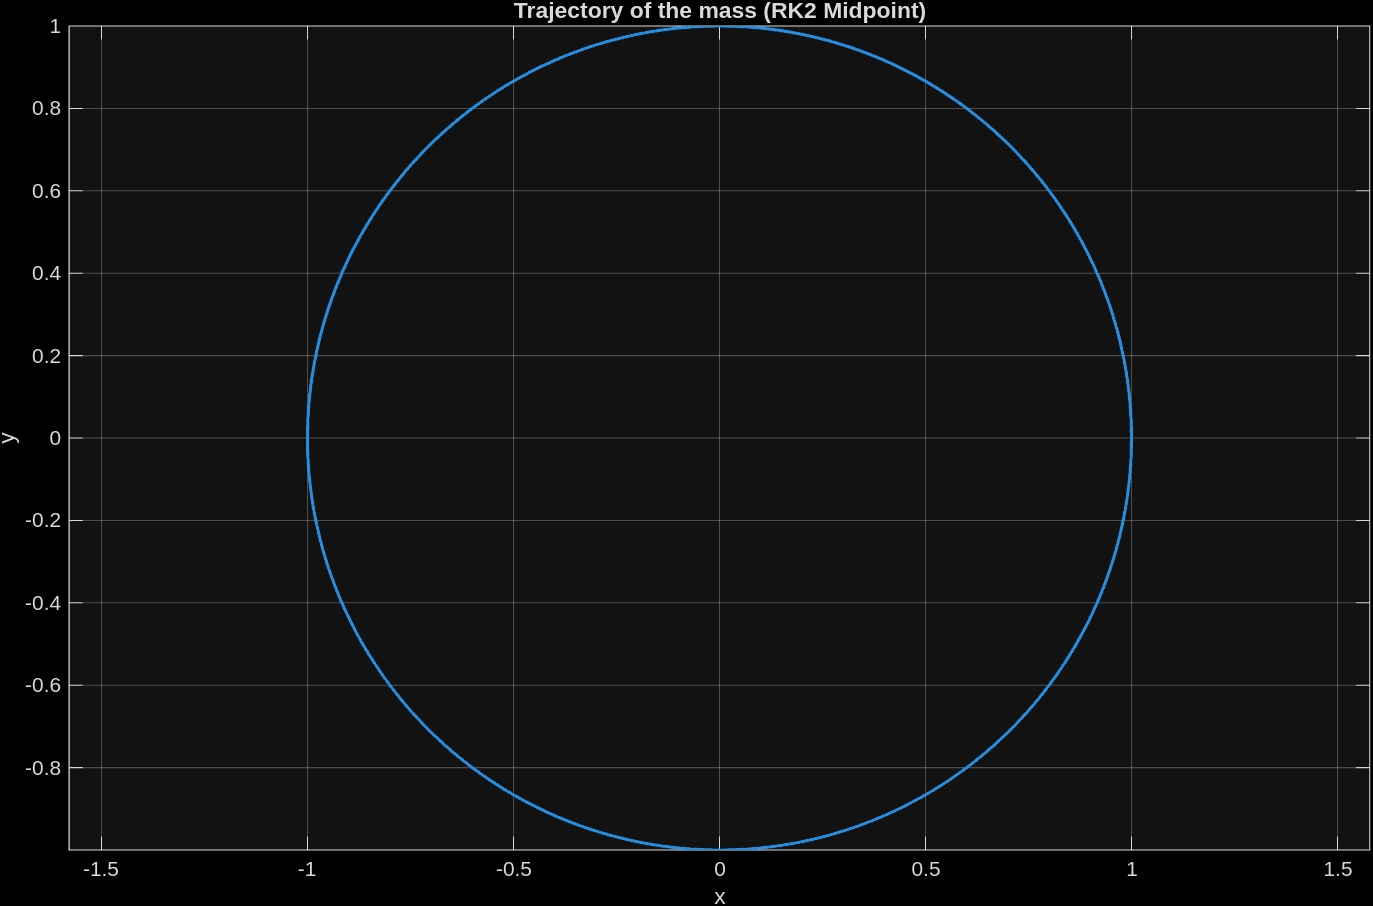
\includegraphics[width=0.5\linewidth]{question7/challenge_circular_motion.png}
    \caption{Observed Circular Motion when $k = 1.0$, $m = 1.0$, $\vec{v}_0 = 1.0\; \hat{j}$ and $\vec{r} = 1.0 \; \hat{i}$}
    \label{fig:placeholder}
\end{figure}


\section{The Trajectory of a Cannon Ball}

The equations of motion of the system are 
\begin{align}
\ddot{x} &= -k \dot{x} \\
\ddot{y} &= -g - k \dot{y}
\end{align}

where $k = \frac{c_d}{m}$.\\
\\

In state-space form, where $u=[x,y,\dot{x},\dot{y}]^\text{T}$, the system is defined as:
\begin{equation}
\frac{d}{dt} \begin{bmatrix} x \ y \ v_x \ v_y \end{bmatrix} = \begin{bmatrix} v_x \ v_y \ -k v_x \ -g - k v_y \end{bmatrix}
\end{equation}

One may derive explicit solutions for the position of the projectile.

\begin{align}
x(t) &= \frac{v_{x0}}{k} \left( 1 - e^{-kt} \right) \\
y(t) &= \frac{v_{y0}}{k} \left( 1 - e^{-kt} \right) - \frac{g}{k} \left( t - \frac{1}{k}(1 - e^{-kt}) \right)
\end{align}

\begin{minted}{julia}
# ===== Engineering Mathematics -- Homework 3, Question 8 ===== #
# Author: Esraaj Sarkar Gupta
# Date: 15th February, 2026

using DifferentialEquations
using LinearAlgebra
using Plots

# --- Define Parameters --- #
m   = 1
θ   = pi/4
v₀  = 10
g   = 1
c   = 1

k = c/m

t_final = 20

t = range(.0, t_final; length=1000)

# --- Initial Conditions --- #
x₀, y₀ = .0, .0
vx₀ = v₀ * cos(θ)
vy₀ = v₀ * sin(θ)

# ===== Part A ===== #
# I have solved for the system analytically, I may not be correct,
# but I have tried.

function projectile_analytic(t, vx₀, vy₀, k, g)
    x = (vx₀ / k) * (1 - exp(-k * t))
    y = (vy₀ / k) * (1 - exp(-k * t)) - (g / k) * (t - (1 / k) * (1 - exp(-k * t)))
    return x, y
end

results = projectile_analytic.(t, vx₀, vy₀, k, g)
x_analytic = [r[1] for r in results]
y_analytic = [r[2] for r in results]

idx_ground = findfirst(val -> val < 0, y_analytic[2:end]) + 1
stop_at = isnothing(idx_ground) ? length(y_analytic) : idx_ground

x_analytic_sliced = x_analytic[1:stop_at]
y_analytic_sliced = y_analytic[1:stop_at]

trajectory = plot(x_analytic_sliced, y_analytic_sliced, aspect_ratio=:equal,  xlabel="x", ylabel="y", label="analytic solution")

# ===== Part B ===== #

# State u = [x, y, dx, dy]
function projectile!(du, u, p, t)
    # Unpack parameter vector
    m, c, g = p

    k = c/m # For convinience

    # Unpack state vector
    x, y, dx, dy = u

    ddy = (- g) + (-k * dy)
    ddx = -k * dx

    du[1] = dx
    du[2] = dy
    du[3] = ddx
    du[4] = ddy
end

# -- Initial Conditions -- #

u₀  = [x₀, y₀, vx₀, vy₀]
tspan = (.0, t_final)

# Parameter Vector
p = (m, c, g)

# Callback conditon -- stop when y = 0 (hits the floor)

condition(u, t, integrator) = u[2]
affect!(integrator) = terminate!(integrator)
cb = ContinuousCallback(condition, affect!)

problem = ODEProblem(projectile!, u₀, tspan, p)
sol = solve(problem, Tsit5(), callback = cb)

x_solutions = sol[1,:]
y_solutions = sol[2,:]
times = sol.t

plot!(trajectory, x_solutions, y_solutions,aspect_ratio=:equal, xlabel="x (m)", ylabel="y (m)", label="numerical solution")
display(trajectory)

# ===== Part C ===== #

# Evaluate the analytical solution at (t=2)
state_at_2 = [projectile_analytic(2, vx₀, vy₀, k, g)...]
errors = []

tolerances = 10 .^ range(-3, -16, length=20)

for tol in tolerances
    temp_sol = solve(problem, Tsit5(), callback=cb, reltol=tol, abstol=tol)
    
    u_num = temp_sol(2.0)
    pos_num = [u_num[1], u_num[2]]
    
    push!(errors, norm(pos_num - state_at_2))
end

plot(tolerances, errors, 
     xscale=:log10, yscale=:log10, 
     marker=:circle, 
     xlabel="Tolerance", ylabel="Error at t=2",
     title="Convergence Study", flipx=true)
\end{minted}

\begin{figure}[htbp]
     \centering
     % --- Row 1 ---
     \begin{subfigure}[b]{0.45\textwidth}
         \centering
         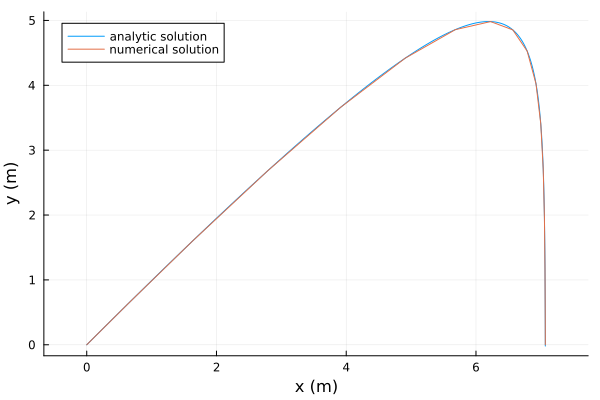
\includegraphics[width=\textwidth]{question8/unremarkable_trajectory.png}
         \caption{Numerical and Analytical Solutions}
         \label{fig:placeholder}
     \end{subfigure}
     \hfill
     \begin{subfigure}[b]{0.45\textwidth}
         \centering
         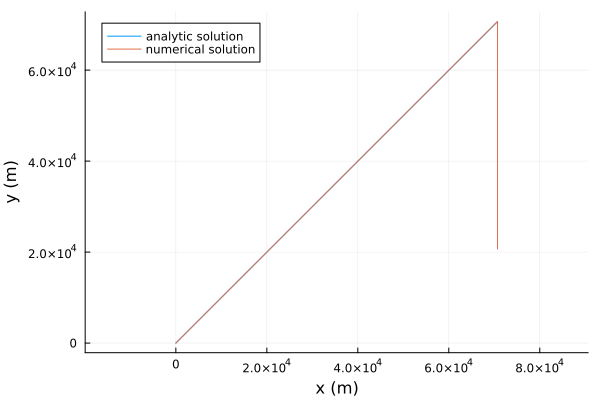
\includegraphics[width=\textwidth]{question8/large_v.png}
         \caption{Trajectory as $v \xrightarrow{} \infty$}
         \label{fig:placeholder}
     \end{subfigure}

    \caption{Projectile Trajectories}
\end{figure}

\begin{itemize}
    \item \textbf{Trajectory Matching:} The numerical solution using the \texttt{Tsit5()} integrator shows high visual agreement with the analytical solution. The use of a \texttt{ContinuousCallback} successfully terminates the simulation at the precise moment of ground impact (y=0).
    
    \item \textbf{Convergence:} The error at t=2 was evaluated against varying tolerances. The resulting log-log plot demonstrates that as the local error tolerances (abstol,reltol) are tightened, the global error decreases linearly on a logarithmic scale, confirming the stability and consistency of the solver.
\end{itemize}

\begin{figure}[h!]
    \centering
    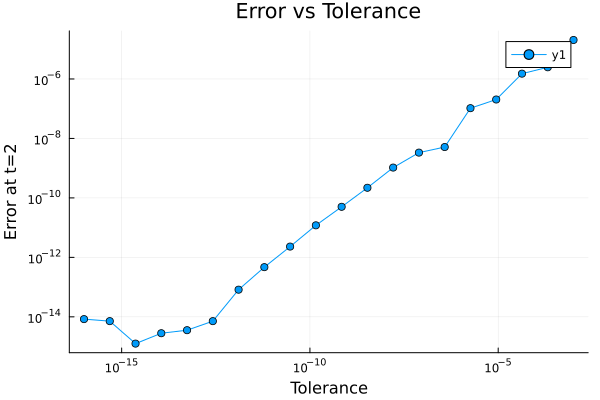
\includegraphics[width=0.5\textwidth]{question8/error_tol.png}
    \caption{}
\end{figure}

\section{Statics vs Dynamics of a Spring-Damper Mass System}

he system consists of a point mass $m$ located at position $\vec{r}_C = [x, y]^\top$. 
Gravity $g$ acts in the downward direction, denoted as $-g\hat{j}$. 

Two anchor points, $A$ and $B$, are fixed at $\vec{r}_A$ and $\vec{r}_B$, respectively. 
The mass is connected to each anchor by a spring and a dashpot arranged in parallel:
\begin{itemize}
    \item \textbf{Anchor A:} Connected via a spring with constant $k_A$ and rest length $L_A$, and a parallel dashpot with damping coefficient $c_A$.
    \item \textbf{Anchor B:} Connected via a spring with constant $k_B$ and rest length $L_B$, and a parallel dashpot with damping coefficient $c_B$.
\end{itemize}

Additionally, the mass is subject to an atmospheric drag force proportional to its speed through the air, characterized by the damping coefficient $c_d$. 

The dynamic state of the system is described by the vector $z = [x, y, v_x, v_y]^\top$, while the static equilibrium state is defined by $z = [x, y, 0, 0]^\top$.

The system may be described using Newton's Second Law of Motion with the vector equation

\begin{equation}
    m \frac{d^2\vec{r}_c}{dt^2} = -mg\hat{j} + \left[ k_A\delta_A + c_A \left( \frac{d\vec{l}_A}{dt} \cdot \hat{a} \right) \right] \hat{a} + \left[ k_B \delta_B + c_B \left( \frac{d\vec{l}_B}{dt} \cdot \hat{b} \right) \right] \hat{b} - c_d \frac{d\vec{r}_c}{dt}  
    \label{Eq:System9}
\end{equation}

where

\begin{eqnarray}
    \vec{r}_c & = & \vec{r}_{A/B} + \big( \vec{L}_{A/B} + \vec\delta_{A/B} \big) \\
    \vec{l}_{A/B} & = & \vec{L}_{A/B} + \vec\delta_{A/B} \nonumber \\
    \vec{a} & = & \vec{r}_c - \vec{r}_A \nonumber \\
    \vec{b} & = & \vec{r}_c - \vec{r}_B \nonumber
    \label{Eq:System9_helper}
\end{eqnarray}

and any vector $\vec{v} = ||v|| \; \hat{v}$.

In the static limit, this equation simplifies to 

\begin{equation}
    mg \; \hat{j} = k_A\delta_A \; \hat{a} + k_B\delta_B \; \hat{b}.
\end{equation}

\begin{minted}{julia}
function get_dparameters(sys::fparameters, r_c::Vector{Float64})
    a_vec = sys.rₐ - r_c
    b_vec = sys.rᵦ - r_c
    
    # Current scalar lengths
    lₐ_val = norm(a_vec)
    lᵦ_val = norm(b_vec)
    
    return dparameters(lₐ_val, lᵦ_val, a_vec, b_vec)
end

# ---- Define System Evolution ---- #

function spring_damper_mass_system!(du, u, p, t)
    # Unpack state
    r_c = u[1:2]
    v_c = u[3:4]

    # Unpack Parameters
    m = p.m 
    r_A, r_B = p.rₐ, p.rᵦ

    k_A, k_B = p.kₐ, p.kᵦ
    L_A, L_B = p.Lₐ, p.Lᵦ

    c_A, c_B, c_d = p.cₐ, p.cᵦ, p.c_d

    # -- Geometry -- #
    vec_to_A = r_A - r_c
    vec_to_B = r_B - r_c

    dist_A = norm(vec_to_A)
    dist_B = norm(vec_to_B)

    # Unit Vectors
    hat_A = vec_to_A / dist_A
    hat_B = vec_to_B / dist_B

    # -- Force Calculations -- #

    # - Springs - #
    delta_A = dist_A - L_A
    delta_B = dist_B - L_B
    
    F_spring_A = k_A * delta_A * hat_A
    F_spring_B = k_B * delta_B * hat_B

    # - Dampers - #
    vel_proj_A = dot(v_c, -hat_A)
    vel_proj_B = dot(v_c, -hat_B)

    F_damp_A = -c_A * dot(v_c, hat_A) * hat_A 
    F_damp_B = -c_B * dot(v_c, hat_B) * hat_B
    
    # - Drag - #
    F_drag = -c_d * v_c

    # - Gravity - #
    F_gravity = [0.0, -m * g]

    # -- Newton's Second Law -- #

    F_total = F_spring_A + F_spring_B + F_damp_A + F_damp_B + F_drag + F_gravity
    accel = F_total / m

    # -- Update State -- #
    du[1:2] = v_c    # dr/dt = v
    du[3:4] = accel  # dv/dt = F/m

end

# Initial Conditions
u0 = [5.0, 0.0, 0.0, 2.0] 

# Time Span
tspan = (0.0, 50.0)

prob = ODEProblem(spring_damper_mass_system!, u0, tspan, params)
sol = solve(prob, Tsit5(), saveat=0.1)

phase_space = plot(sol, idxs=(1,2), 
     title="Mass Trajectory", 
     xlabel="x position (m)", 
     ylabel="y position (m)", 
     label="Path", lw=2, aspect_ratio=:equal)

# ---- Solving for a Static System ---- #

function static_forces!(F, r_c, sys::fparameters)
    a_vec = sys.rₐ - r_c
    b_vec = sys.rᵦ - r_c
    
    lₐ = norm(a_vec)
    lᵦ = norm(b_vec)
    
    hat_a = a_vec / lₐ
    hat_b = b_vec / lᵦ
    
    delta_a = lₐ - sys.Lₐ
    delta_b = lᵦ - sys.Lᵦ
    
    gravity = [0.0, -sys.m * g]
    force_a = sys.kₐ * delta_a * hat_a
    force_b = sys.kᵦ * delta_b * hat_b
    
    # Update the F array in-place
    F[1] = gravity[1] + force_a[1] + force_b[1] 
    F[2] = gravity[2] + force_a[2] + force_b[2] 
end

# ---- Generate Steady State Solution Clusters ---- #

num_samples = 2000
solutions_x = Float64[]
solutions_y = Float64[]

# Wrap the function so NLsolve only sees F and x
target_func!(F, x) = static_forces!(F, x, params)

for i in 1:num_samples
    x0 = -5.0 + 20.0 * rand()
    y0 = -10.0 + 25.0 * rand()
    initial_guess = [x0, y0]
    
    
    res = nlsolve(target_func!, initial_guess, autodiff=:forward, ftol=1.5)
    
    # If successful, save the raw, unrounded coordinates
    if converged(res)
        push!(solutions_x, res.zero[1])
        push!(solutions_y, res.zero[2])
    end
end


# ---- Custom Steady State Clustering Algorithm ---- #
# Combine points for easier handling
points = tuple.(solutions_x, solutions_y)

# Round off to integers and find unique classes
rounded_points = tuple.(round.(Int, solutions_x), round.(Int, solutions_y))
unique_classes = unique(rounded_points)

println("Identified $(length(unique_classes)) integer class seeds.")

# Create a dictionary to hold the assigned points for each class
clusters = Dict(c => Tuple{Float64, Float64}[] for c in unique_classes)

# Assign each original point to the nearest integer class using Euclidean distance
for p in points
    best_class = unique_classes[1]
    min_dist = Inf
    
    for c in unique_classes
        # Euclidean distance formula
        dist = sqrt((p[1] - c[1])^2 + (p[2] - c[2])^2)
        if dist < min_dist
            min_dist = dist
            best_class = c
        end
    end
    push!(clusters[best_class], p)
end

# Centroids of each newly formed class
centroids_x = Float64[]
centroids_y = Float64[]

for (class_seed, cluster_points) in clusters
    if !isempty(cluster_points)
        # Calculate mean of X and Y
        cx = sum(p[1] for p in cluster_points) / length(cluster_points)
        cy = sum(p[2] for p in cluster_points) / length(cluster_points)
        
        push!(centroids_x, cx)
        push!(centroids_y, cy)
        
        println("Region Centroid: (X: $(round(cx, digits=4)), Y: $(round(cy, digits=4)))")
    end
end
\end{minted}

Solving for this system using a 5th order solver (TSit), one may observe obvious signs of a chaotic system

\begin{itemize}
    \item Sensitivity to initial conditions.
    \item Strange attractors in the phase space (clearly visible)
    \item Open loops (aperiodicity) in the phase space.
\end{itemize}

\begin{figure}[!h]
    \centering
    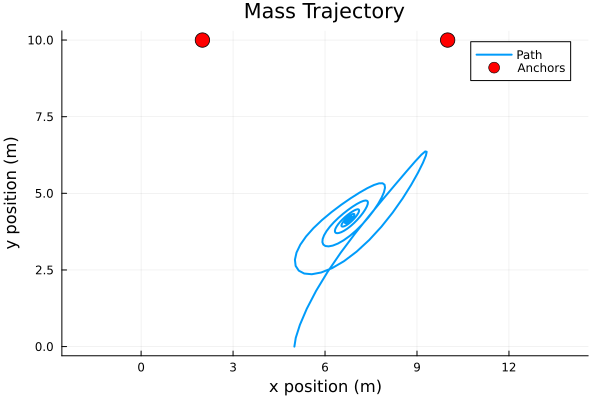
\includegraphics[width=0.8\linewidth]{question9/chaos1.png}
    \caption{TSit Numerical Solution -- Phase Space}
    \label{fig:placeholder}
\end{figure}

One may use Julia's NLsolve (similar to MatLab's fsolve) to identify the system's static solutions. The system is reduced to its static limit and fed into NLsolve, which identified 1737 (unique and non-unique) solutions in 2000 runs. \\
\\

\begin{figure}[!h]
    \centering
    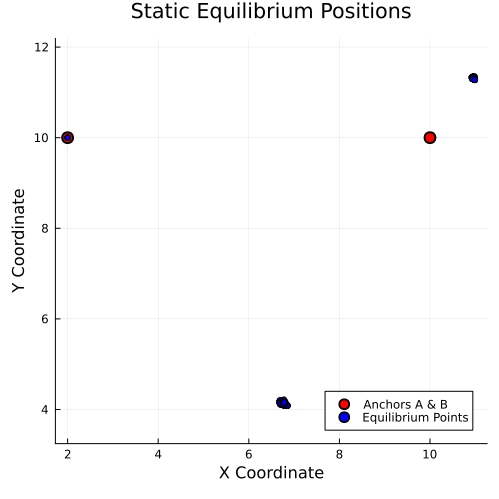
\includegraphics[width=0.4\linewidth]{question9/static_solutions.png}
    \caption{NLsolve Solutions}
    \label{fig:placeholder}
\end{figure}

One can clearly visualize that the solutions are far apart. Given the nature of the clusters, one may forgo using standard clustering algorithms in machine learning (such as KMeans or GMM) in place of much simpler algorithms. Here the following algorithm is used to define clusters.

\begin{enumerate}
    \item All solutions are reduced to their greatest integer forms. This can be done this the the error by NLsolve is smaller than $\mathcal{O}(1)$.
    \item Unique (integral) solutions are identified. Each unique solution is assigned an unlabeled class (or cluster) as a \textit{center point}.
    \item All the (unrounded) solutions from NLsolve are assigned a cluster based on the least Euclidean distance from the respective \textit{center point}.
    \item The centroid of all the points in each cluster is presented a point of equillibrium.
\end{enumerate}

\begin{figure}[h!]
    \centering
    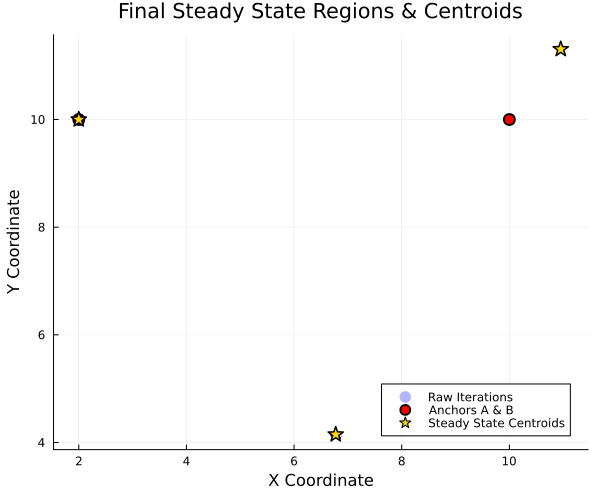
\includegraphics[width=0.4\linewidth]{question9/rounded_static_solutions.png}
    \caption{Clustered NLsolve Solutions for System Statics}
    \label{fig:placeholder}
\end{figure}

\begin{table}[htbp]
    \centering
    \caption{Final Steady State Regions (Centroids)}
    \label{tab:steady_state_centroids}
    \begin{tabular}{ccc}
        \hline
        \textbf{Region} & \textbf{X Coordinate (m)} & \textbf{Y Coordinate (m)} \\
        \hline
        1 & 6.7738 & 4.1472 \\
        2 & 2.0000 & 10.0000 \\
        3 & 10.9523 & 11.3063 \\
        \hline
    \end{tabular}
\end{table}

To evaluate the stability of the discovered fixed points, one may simulate the system with initial positions set to the fixed points and an arbitrarily small velocities to simulate a perturbation. Observing the behaviour of the system (converging back to the fixed point/ diverging from the fixed point) allows one to assess the stability.

In the system simulate here, three distinct fixed points were discovered. The system was simulated (as done above) using TSit5 from the fixed points with varying perturbations. It is discovered that two of the three fixed points are unstable. Following their respective perturbations, all three masses converge at the singular stable fixed point of the system.

\begin{figure}
    \centering
     % --- Row 1 ---
     \begin{subfigure}[b]{0.45\textwidth}
         \centering
         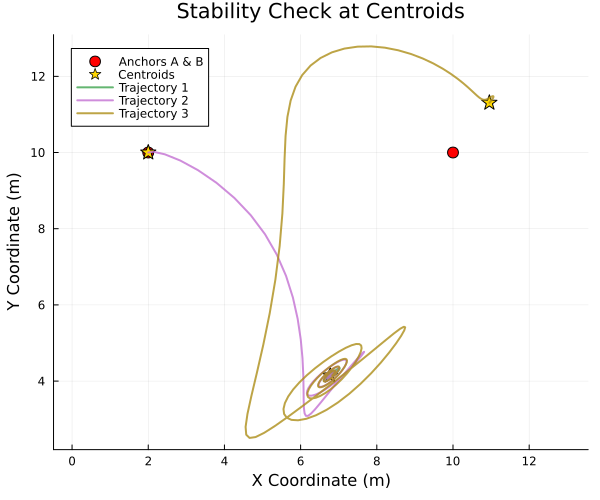
\includegraphics[width=\textwidth]{question9/stability.png}
         \caption{Perturbation of $\vec{v}_0 = (0.5 \;\hat{i}+ 0.5 \;{\hat{j})}\; \text{m/s}$}
         \label{fig:k0}
     \end{subfigure}
     \hfill
     \begin{subfigure}[b]{0.45\textwidth}
         \centering
         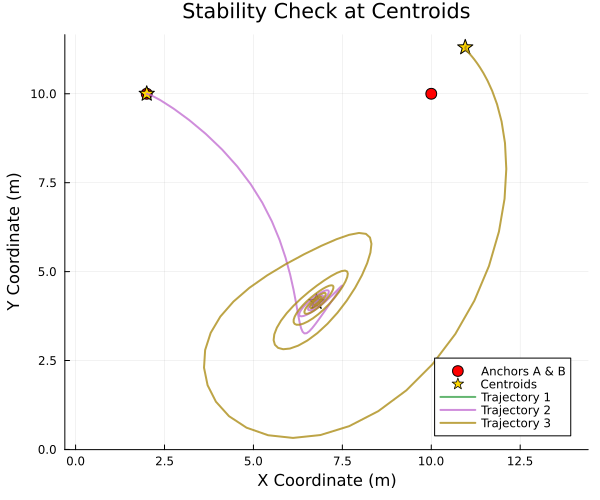
\includegraphics[width=\textwidth]{question9/stability2.png}
         \caption{Perturbation of $\vec{v}_0 = (0.1 \;\hat{i}+ 0.1 \;{\hat{j})}\; \text{m/s}$}
         \label{fig:rigid}
     \end{subfigure}

    \caption{Stability of Discovered Fixed Points}
\end{figure}

\section{Linear Ordinary Differential Equations}

It is useful to consider the solution to any linear ODE to be of the form $x(t) = Ce^{\lambda t}$ where $\lambda \in \mathbb{C}$. The general solution of linear ODEs is given as a linear combination of any solutions to the same ODE. Given a coupled system of linear differential equations

\begin{equation}
    \dot{X} = AX
\end{equation}

one may consider the solution of $X$ to be of the form 

\begin{equation}
    X = e^{\lambda t}v
\end{equation}

where $v$ is some arbitrary vector of the same dimensions. Thus,

\begin{equation}
    \dot{X} = \lambda e^{\lambda t}v.
\end{equation}

This yields the eigenvalue-eigenvector equation

\begin{equation}
    \lambda v = Av.
\end{equation}

The general solution of such a system is of the form

\begin{equation}
    X(t) = c_1 e^{\lambda t} + c_2 e^{\lambda t} + \dots
\end{equation}

which is used to solve the initial value problem $X_0 = X(t=0)$.

\begin{equation}
    X_0 = c_1v_1 + c_2v_2 + \dots
\end{equation}.

Considering an example system of 

\begin{equation}
    A = 
    \begin{pmatrix}
        3 & 1 \\
        1 & 3
    \end{pmatrix}
    \qquad X_0 =
    \begin{pmatrix}
        5 \\
        0
    \end{pmatrix}
\end{equation}

this analytical solution to compared to the solution obtained from a 5$^\text{th}$ order numerical solver.

\begin{figure}
    \centering
    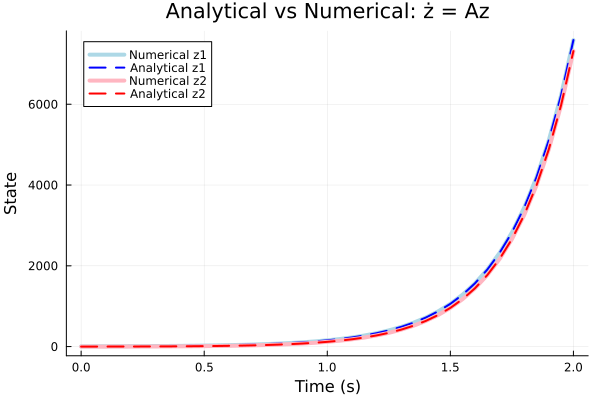
\includegraphics[width=0.5\linewidth]{question10/linear_ODEs.png}
    \caption{Linear ODEs: Numerical vs Analytical Solutions}
    \label{fig:placeholder}
\end{figure}

\section{Revisiting the Spring-Mass Damper System -- Analysis of Linear Stability}

The animation of the dynamics of the system is improved. Damped springs are animated (with great difficulty). The system is simulated with various parameters and various initial conditions.

\begin{figure}[h!]
    \centering
    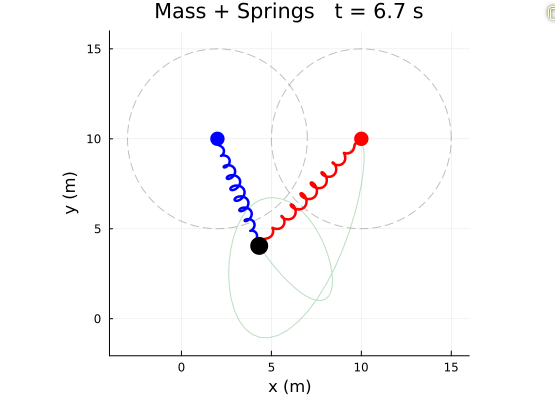
\includegraphics[width=0.5\linewidth]{question11/animated_springs_example.png}
    \caption{Animated Springs Example}
    \label{fig:placeholder}
\end{figure}

\begin{minted}{julia}
function get_spring_coords(p1, p2; R=0.35, coils=12, points=200, tilt=0.6)
    v = p2 - p1
    L = norm(v)
    
    # Unit vectors (axial and normal)
    u = v / (L + 1e-6)
    n = [-u[2], u[1]]
    
    xs = zeros(points)
    ys = zeros(points)
    
    t_vals = range(0, 1, length=points)
    for (i, t) in enumerate(t_vals)
        # Angle parameter for the helix
        theta = coils * 2π * t
        
        # Taper envelope to make ends connect cleanly to the points
        env = sin(π * t) 
        
        # Calculate offset in 3D and project to 2D
        # tilt controls how much the out-of-plane loop overlaps in 2D
        u_dist = L * t + (R * tilt * env) * sin(theta)
        n_dist = (R * env) * cos(theta)
        
        pos = p1 .+ u_dist .* u .+ n_dist .* n
        xs[i] = pos[1]
        ys[i] = pos[2]
    end
    
    return xs, ys
end

\end{minted}

\begin{figure}[!h]
    \centering
    % First subfigure
    \begin{subfigure}[b]{0.45\textwidth}
        \centering
        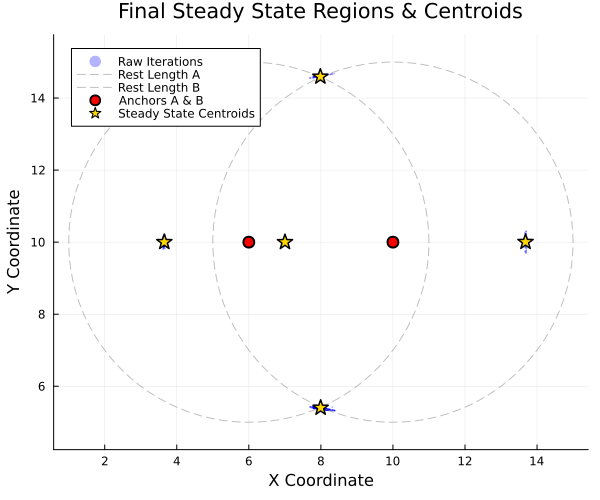
\includegraphics[width=\textwidth]{question11/compression.png}
        \caption{Anchors placed closer to each other than $L_A + L_B$}
        \label{fig:compression}
    \end{subfigure}
    \hfill
    % Second subfigure
    \begin{subfigure}[b]{0.45\textwidth}
        \centering
        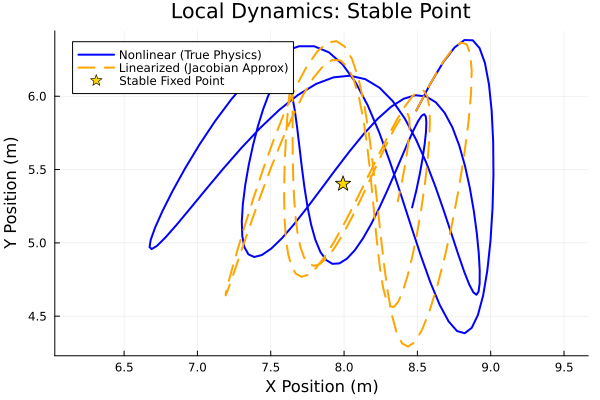
\includegraphics[width=\textwidth]{question11/compression_linear.png}
        \caption{System linearized about the fixed point.}
        \label{fig:compression_linear}
    \end{subfigure}
    
    \caption{Overall comparison of the two compression states}
    \label{fig:compression_combined}
\end{figure}

\begin{mdframed}[backgroundcolor=gray!10]
    \textbf{Careless Programming:}\\
    While carrying out the analysis of equilibria near the anchors, a critical zero-division bug in the code defining the system is identified. Specifically in the lines \texttt{hat\_A = vec\_to\_A / dist\_A} and \texttt{hat\_B = vec\_to\_B /dist\_B}. If the object happens to be placed at the same point as one of the anchors, the corresponding distances vanish. This error is fixed by introducing a small term $\epsilon = 10^{-6}$ in the denominators.
\end{mdframed}

\subsection{Why do fixed points show up frequently near anchors?}

One may assert that the neighborhoods of the anchors generally present more fixed points. The rationale for this assertion is as follows. Springs generate the largest compressive force possible at their respective anchors, and with a expansion vector with an undefined direction $\hat\delta = \frac{\vec\delta}{0}$, the repulsive spring force is awarded an extra degree of freedom , allowing it to point in any direction. This extra degree of freedom makes these points more likely to be equilibria, although always unstable. Examples of this phenomenon are demonstrated in Fig. \ref{fig:equilibria_on_anchors}.\\

\begin{equation}
    k_B\delta_B = k_A\delta_A\sin(\theta)
\end{equation}

where $\theta$ can be anything (extra degree of freedom). $\delta_A$ is arbitrarily small. 

\begin{figure}[htbp]
     \centering
     \begin{subfigure}[b]{0.45\textwidth}
         \centering
         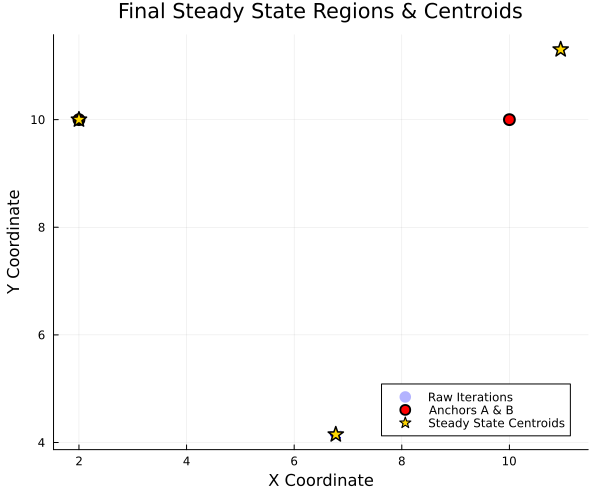
\includegraphics[width=\textwidth]{question11/anchor_equillibira_1.png}
         \caption{}
         \label{fig:}
     \end{subfigure}
     \hfill
     \begin{subfigure}[b]{0.45\textwidth}
         \centering
         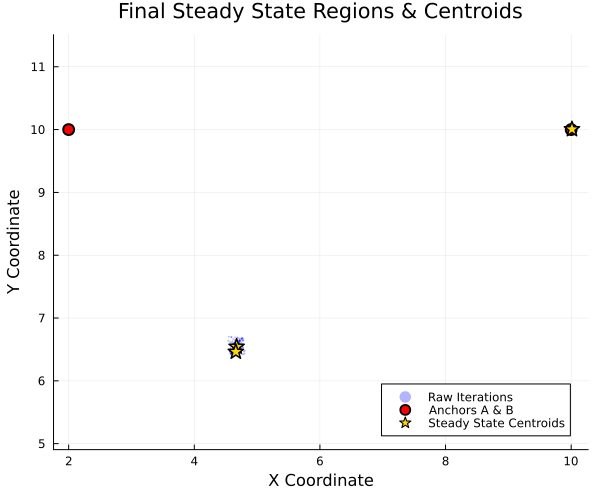
\includegraphics[width=\textwidth]{question11/anchor_equillibira_2.png}
         \caption{}
         \label{fig:}
     \end{subfigure}
        \caption{Examples of fixed points coinciding with the anchors.}
        \label{fig:equilibria_on_anchors}
\end{figure}

\subsection{Linearization}
One may use the Jacobian of a system to linearize it about a point. Here the system is linearized about identified stable and unstable fixed points. The nature of fixed points may be determined by analyzing the eigenvalues of the Jacobian matrix at the fixed point.

\begin{equation}
    \dot{\delta u} = J(u^*)\;\delta u \label{Eq:jacobian}
\end{equation}

While the root-finder \texttt{fsolve} from MATLAB directly allows the user to extract the Jacobian generated at runtine, Julia's root-finder \texttt{NLsolver} does not provide such convenience. Instead, to compute the Jacobian in Julia, the package \texttt{ForwardDiff} is used.\\
\\
The fixed points of the system were identified, and both stable and unstable fixed points were linearized about. The system was then solved for using a 5$^\text{th}$ order solver (\texttt{Tsit()}) analogous to \texttt{ODE45} and results were compared. It is observed that the linearized system closely follows the true system near stable fixed points, while it diverges rapidly from the unstable fixed points ($\sim 2.5s$).

\begin{figure}[htpb]
    \centering
    \begin{subfigure}[b]{0.45\textwidth}
        \centering
        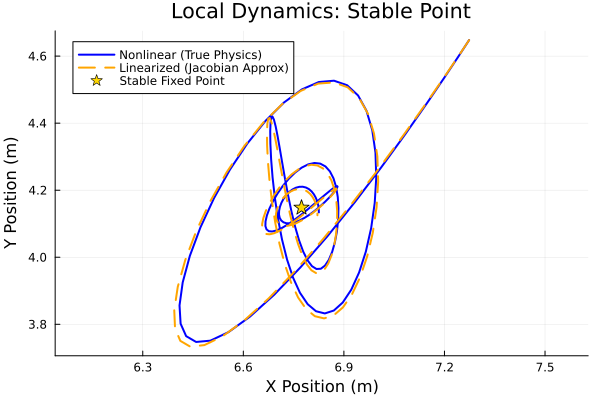
\includegraphics[width=\textwidth]{question11/stable_linear_vs_non_linear.png}
        \caption{Stable Fixed Point}
    \end{subfigure}
    \hfill
    \begin{subfigure}[b]{0.45\textwidth}
        \centering
        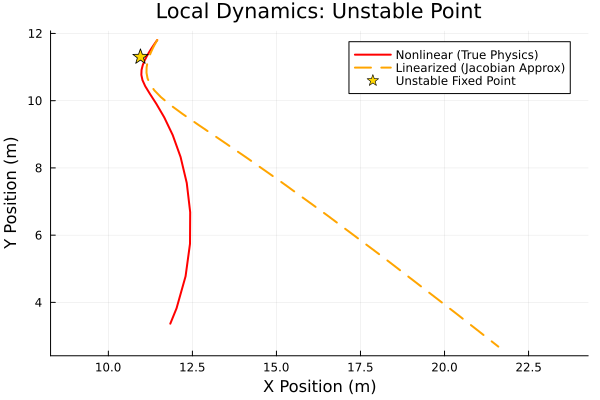
\includegraphics[width=\textwidth]{question11/unstable_linear_vs_non_linear.png}
        \caption{Unstable Fixed Point}
    \end{subfigure}
        \caption{Linear vs Non-Linear Behavior of Fixed Points}
        \label{fig:linear-vs-nonlinear-fixedpoints}
\end{figure}

\begin{table}[h!]
\centering
\small
\begin{tabular}{|c|c|l|l|}
\hline
\textbf{Real ($\alpha$)} & \textbf{Imag ($\beta$)} & \textbf{Type} & \textbf{Stability} \\ \hline
$\alpha < 0$ & $\beta = 0$ & Stable Node & Attracting \\ \hline
$\alpha < 0$ & $\beta \neq 0$ & Stable Focus & Attracting \\ \hline
Mixed Signs & Any & Saddle Point & Unstable \\ \hline
$\alpha > 0$ & $\beta = 0$ & Unstable Node & Repelling \\ \hline
$\alpha > 0$ & $\beta \neq 0$ & Unstable Focus & Repelling \\ \hline
$\alpha = 0$ & $\beta \neq 0$ & Center & Marginally Stable \\ \hline
\end{tabular}
\caption{Fixed Point Classification ($\lambda = \alpha \pm \beta i$)}
\label{tab:eigenvalue_classification}
\end{table}

\newpage
\begin{minted}{julia}

# ---- Linearization about Fixed Points ---- #
# -- Define Common Parameters -- #
tspan_s = (0.0, 15.0)
tspan_u = (0.0,  2.0)
δu0 = [0.5, 0.5, 1.0, 2.0] # State Offset

# -- Linearization and Plot Block -- #
# ---- Linearization about Fixed Points ---- #

# Define linearized ODE function
function linearized_system!(du, u, p, t)
    J_matrix = p
    mul!(du, J_matrix, u)
end


# -- Modular Linearization and Plot Function -- #
function linearize_and_plot(
    fixed_point::fixedpoint_properties,
    type_label::String, δu0::Vector{Float64},
    tspan::Tuple{Float64, Float64}, 
    sys_params,
    tcolor::Symbol
    )
    
    # Extract point specific data
    J_point = fixed_point.J_matrix
    u_point = [fixed_point.cx, fixed_point.cy, 0.0, 0.0]

    # State setups
    u0_linear = δu0
    u0_nonlinear = δu0 + u_point

    # --- Simulate Linear --- #
    prob_lin = ODEProblem(linearized_system!, u0_linear, tspan, J_point)
    sol_lin = solve(prob_lin, Tsit5(), saveat=0.1)

    # --- Simulate Nonlinear --- #
    prob_nonlin = ODEProblem(spring_damper_mass_system!, u0_nonlinear, tspan, sys_params)
    sol_nonlin = solve(prob_nonlin, Tsit5(), saveat=0.1) 
\end{minted}

\textbf{Linearization: Special Case, $L_A = L_B = 0$ and $c_A = c_B = 0$}\\
In the special case where both spring rest lengths $L_A$ and $L_B$ are set to zero, and the damping coefficients $c_A$ and $c_B$ are set to zero, the system fails to generate any unstable fixed points. Linearizing about the stable fixed point, it is observed that the linearized system perfectly follows the true (supposedly) non-linear system. To explain this behavior we examine the equations of motion of the system under these constraints.

\begin{equation}
    m \frac{d^2\vec{r}_c}{dt^2} = -mg\hat{j} + k_A l_A \hat{a} + k_B l_B\hat{b} - c_d \frac{d\vec{r}_c}{dt}     
\end{equation}

Consider either of the spring force terms $k_i l_i \hat{i}$. From Eq. \ref{Eq:System9_helper}, we see that $\hat{i} = -\frac{\vec{l}_i}{|l_i|}$. The spring force thus simplifies to

\begin{equation}
    \vec{F} = - k_i \vec{l_i}.
\end{equation}

This equation lacks the non linear term $|l_i| = \sqrt{x_i^2 + y_i^2}$, thus linearizing the system.

\begin{figure}[h!]
    \centering
    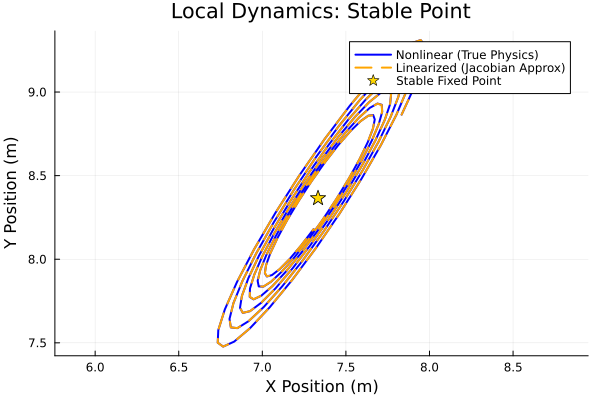
\includegraphics[width=0.5\linewidth]{question11/scase_true.png}
    \caption{$L_A = L_B = c_A = c_B = 0$}
    \label{fig:question11_specialcase}
\end{figure}

\section{Introducing Optimization}

In this problem, numerical optimization is introduced. The surface used here is 

\begin{equation}
    z = (x(x-y))^2 - \exp(-x^2-y^2) - cos(x) \label{intro-optimization-surface}
\end{equation}

subject to the constraints

\begin{eqnarray}
    x + y + \frac{z}{3} = 0 \label{intro-opti-constraint1} \\
    x^2 + y^2 + z^2 = 0. \label{3d_unit_circle-constraint}
\end{eqnarray}

The benchmark optimum is (apparently)  $(x, y, z) \approx (0.236, 0.364, −1.800)$.

\subsection{Grid Search}
The most primitive approach to this problem is to use a grid search and iteratively compute the value of $z$ at every point on the surface and pick the point with the lowest value.

\begin{minted}{julia}
function run_grid_search()
    step = 0.0001
    tol  = 0.001

    X_best = (0.0, 0.0)
    z_min = Inf64

    # Range limits
    r = 1.0
    x_range = -r:step:r
    y_range = -r:step:r

    # ---- Begin Grid Search ---- #
    for x in x_range
        for y in y_range

            if (x^2 + y^2) > r^2
                continue
            end

            z_surface = z(x,y)
            z_plane = p(x,y)

            if abs(z_plane - z_surface) < tol
                if z_plane < z_min
                    z_min = z_plane
                    X_best = (x,y)
                end
            end
        end
    end
    return X_best, z_min
end
\end{minted}

Running the grid search results in a computed minimum of $ (x, y, z) \approx (0.229, 0.371, -1.801)$.

\subsection{Solving Libraries -- Ipopt}
Instead of using a crude grid-search, one may use a large-scale non-linear optimization library such as \texttt{Ipopt} that is available as a Julia package. \texttt{Ipopt} can be used alongside \textit{Julia for Mathematical Programming} \texttt{JuMP}. This is a direct substitue to MATLAB's \texttt{fmincon}.

\begin{minted}{julia}
# ===== Engineering Mathematics -- Homework 4 ===== #
# Author: Esraaj Sarkar Gupta
# Date: 4th April, 2026

using JuMP
using Ipopt

# -- Define Surfaces -- #
# Define optimization surface
z(x,y) = (x * (x-y))^2 - exp(-x^2-y^2) - cos(x)

# Define constraint plane
p(x,y) = -3*(x+y)


function myFmincon()
    # Init optimizer model with Ipopt solver
    model = Model(Ipopt.Optimizer)
    
    # Quiet!
    set_silent(model)

    # Define variables
    @variable(model, -1.0 <= x <= 1.0)
    @variable(model, -1.0 <= y <= 1.0)
    @variable(model, z)

    # Initial guesses
    set_start_value(x, 0.2)
    set_start_value(y, 0.3)
    set_start_value(z, -1.5)

    # Define objective
    @objective(model, Min, z)

    # Define constraints
    @constraint(model, plane, x + y + z/3 == 0)
    
    # The unit circle inequality constraint
    @constraint(model, circle, x^2 + y^2 <= 1.0)
    
    # The surface equality constraint
    @constraint(model, surface, z == (x * (x - y))^2 - exp(-x^2 - y^2) - cos(x))

    # Run!
    optimize!(model)

    return value(x), value(y), value(z), termination_status(model)
end

# Execute the function
x_opt, y_opt, z_opt, status = myFmincon()

println("Solver Status: ", status)
println("Optimal x ≈ ", round(x_opt, digits=3))
println("Optimal y ≈ ", round(y_opt, digits=3))
println("Optimal z ≈ ", round(z_opt, digits=3))
\end{minted}

Ipopt yields a result of $(x,y,z) \approx (0.236, 0.364, -1.8)$.

\section{Basics of Periodic Solutions}

Consider a system defined by the equation of motion

\begin{equation}
    \ddot{\vec{r}} = - \frac{k}{m} \vec{r}.
\end{equation}

Using the same method used earlier, we consider a solution for $\vec{r}$ of the form

\begin{equation}
    \vec{r} = A\exp(\omega t)
\end{equation}

where $i = x,y,z$. Upon equating, one may observe that $A^2 = \sqrt{(-\omega^2)}$. Given that the general solution of any linear second order system can be expressed as the sum of its solutions, the general solution of this problem is arrived at -- a simple harmonic oscillator.

\begin{equation}
    r_i(t) = A_i \cos(\omega t) + B_i \sin(\omega t).
\end{equation}

It is thus evident that any such system has periodic solutions. We may confirm this numerically as is done in Figure \ref{fig:second_order_periodic_numerical_solution}. 

\begin{figure}[h!]
    \centering
    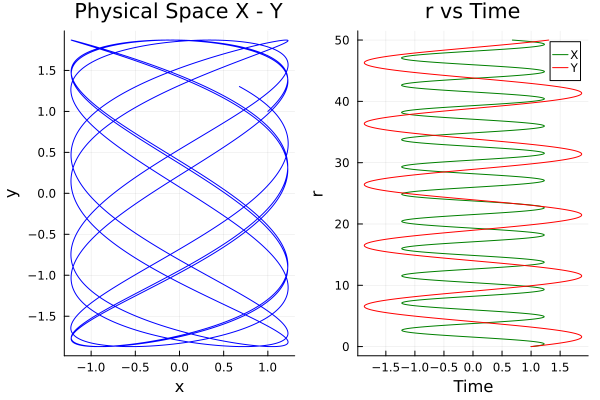
\includegraphics[width=0.5\linewidth]{question13/periodic_solutions.png}
    \caption{Periodic Solutions for Second Order Systems}
    \label{fig:second_order_periodic_numerical_solution}
\end{figure}

\subsection{Inverse Square Central Gravity}
In this section, a special second order system is explored. The Inverse Square Central Gravity system is given by

\begin{equation}
    \ddot\vec{r} = - G\frac{M}{r^3}\vec{r}.
\end{equation}

Despite having a cubed term in its denominator, this system is termed inverse "square" central gravity system since when the vector $\vec{r}$ is decomposed to a magnitude and direction $\vec{r} = r\hat{r}$, the right hand side expression simplifies to $-G\frac{M}{r^2}\hat{r}$.\\
\\
This can be solved analytically, and has been -- as the famous Kepler Problem. Here is it solved numerically using Julia. In the solutions given in Figure \ref{fig:keplers-problem}, it is assumed that $\frac{G}{M} = 10$.

\begin{figure}[h!]
    \centering
    \begin{subfigure}[b]{0.45\textwidth}
        \centering
        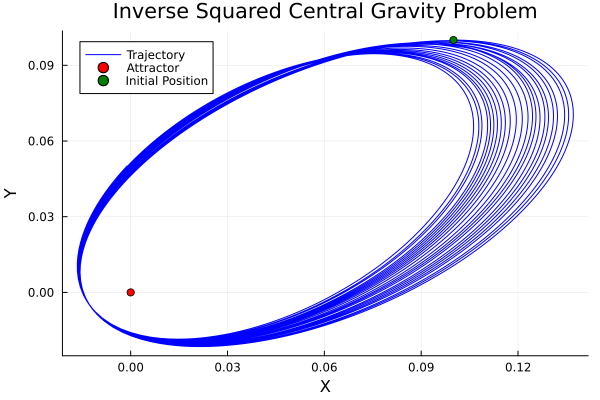
\includegraphics[width=\textwidth]{question13/periodic.png}
        \caption{Periodic Solution ($v_{x0} = 5$ m/s)}
    \end{subfigure}
    \hfill
    \begin{subfigure}[b]{0.45\textwidth}
        \centering
        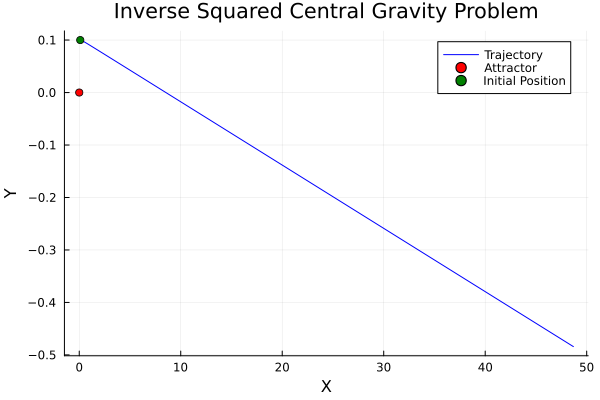
\includegraphics[width=\textwidth]{question13/inf.png}
        \caption{Solution extends to infinity ($v_{x0} = 0.5$) m/s}
    \end{subfigure}
        \caption{Numerical Solutions to Kepler's Problem}
        \label{fig:keplers-problem}
\end{figure}

One can check for numerical inaccuracy in trajectories such as the one presented in Fig. \ref{fig:keplers-problem} by simply reducing the tolerance of the solver and looking out for changes in the suspected inaccuracies. Luckily, when this experiment was carried out for this example, reducing the relative and absolute tolerances to \texttt{1e-8} yields a near-perfect solution.

\begin{figure}[htbp]
    \centering
    % First subfigure
    \begin{subfigure}[b]{0.45\textwidth}
        \centering
        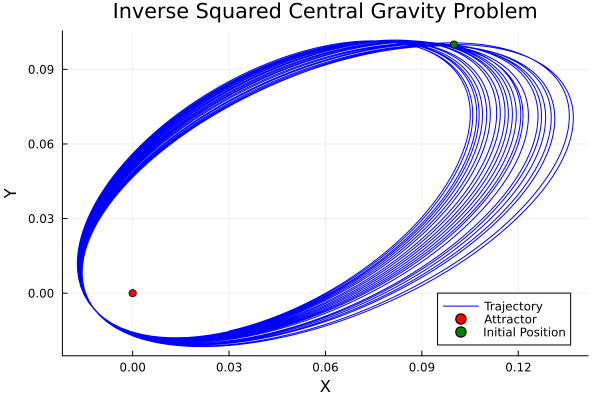
\includegraphics[width=\textwidth]{question13/1em3.png} 
        \caption{\texttt{tol = 1e-3}}
        \label{fig:sub1}
    \end{subfigure}
    \hfill
    \begin{subfigure}[b]{0.45\textwidth}
        \centering
        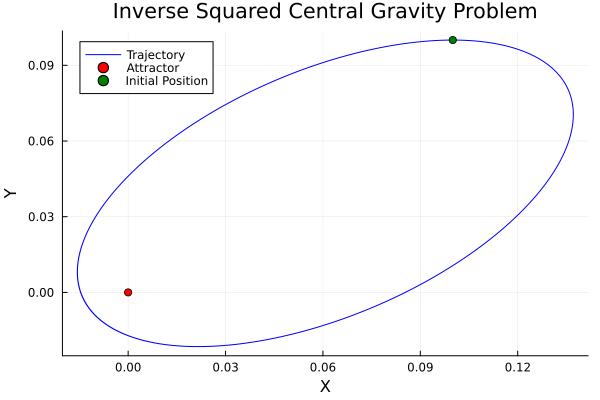
\includegraphics[width=\textwidth]{question13/1em8.png} 
        \caption{\texttt{tol = 1e-8}}
        \label{fig:sub2}
    \end{subfigure}
    
    \caption{Experiment to check for numerical inaccuracies}
    \label{fig:tolerance_comparison}
\end{figure}

\subsection{General Non-Linear Second Order Systems}

 The systems thus covered in this section may be generalized with the equation

\begin{equation}
    \ddot{\vec{r}} = -k r^{n-1} \vec{r}.
\end{equation}

In the special case where the system initially has no velocity and $k_X = k_y$, one may observe that the system propagates as a straight line. This can be visualised in Figure \ref{fig:question13_straightlines}.

\begin{figure}[h!]
    \centering
    % --- Top Row ---
    \begin{subfigure}[b]{0.48\textwidth}
        \centering
        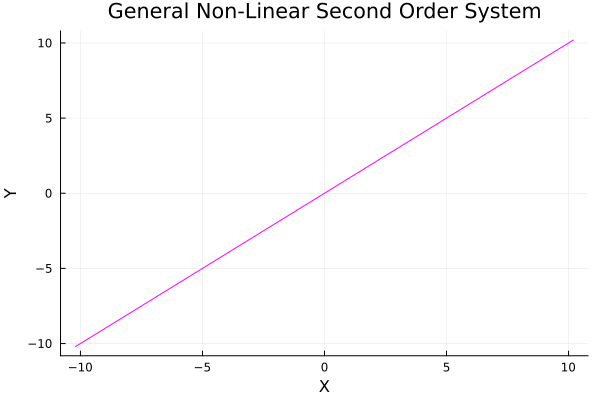
\includegraphics[width=\textwidth]{question13/nonLinear_secondOrder_3n.png}
        \caption{$n=3$}
        \label{fig:sub1}
    \end{subfigure}
    \hfill
    \begin{subfigure}[b]{0.48\textwidth}
        \centering
        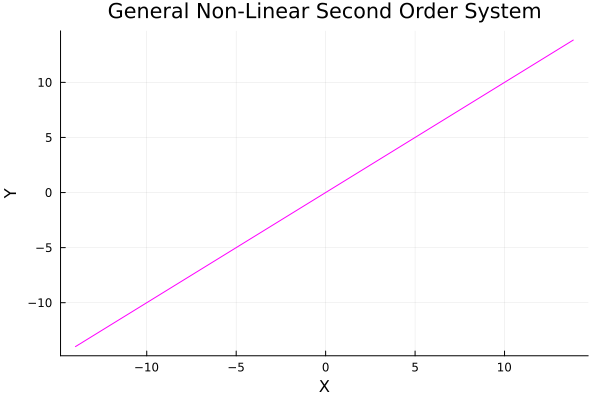
\includegraphics[width=\textwidth]{question13/nonLinear_secondOrder_5n.png}
        \caption{$n=5$}
        \label{fig:sub2}
    \end{subfigure}

    \vspace{0.5cm} % Adds vertical spacing between rows

    % --- Bottom Row ---
    \begin{subfigure}[b]{0.48\textwidth}
        \centering
        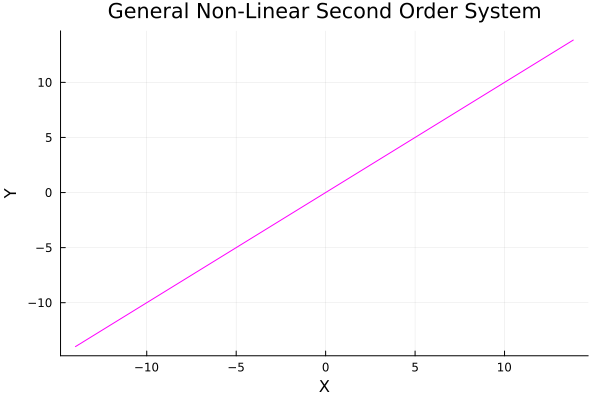
\includegraphics[width=\textwidth]{question13/nonLinear_secondOrder_10n.png}
        \caption{$n=10$}
        \label{fig:sub3}
    \end{subfigure}
    \hfill
    \begin{subfigure}[b]{0.48\textwidth}
        \centering
        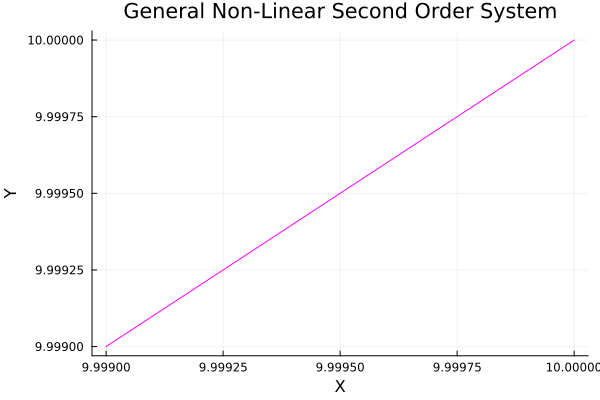
\includegraphics[width=\textwidth]{question13/nonLinear_secondOrder_m5n.png}
        \caption{$n=-5$}
        \label{fig:sub4}
    \end{subfigure}

    \caption{Results for any $n$ under the conditions $k_X = k_y$ and $\dot{r} = 0$}
    \label{fig:question13_straightlines}
\end{figure}

\vfill

\subsection{Using Root-Finding methods to Indetify Periodic Solutions}
A solution $u(t)$ is said to be periodic if, for an arbitrary $T$, it satisfies the condition

\begin{equation}
    u(0) = u(T).
\end{equation}

One may treat this as a Boundary Value Problem, with the condition that the initial value must be equal to the final value. Formally, this approach is known as the shooting method. The \textit{Flow Map} $\Phi_t(x_0) = x(t)$ is used to define the \textit{Shooting Function} $G(u_0, T)$.
\begin{minted}{julia}
# ---- Looking for a Periodic Solution ---- #
# Using the Shooting Function Method
x_fixed = 0.0 # Poincare Manifold

function shooting_residual!(F, vars)
    # Unpack guesses
    y_guess, vx_guess, vy_guess, T_guess = vars

    # Force x = 0.0 (Poincare Manifold)
    u_start = [x_fixed, y_guess, vx_guess, vy_guess]

    # Tight tolerance solving
    prob_shoot = ODEProblem(spring_damper_mass_system!, u_start, (0.0, T_guess), params)
    sol_shoot = solve(prob_shoot, Tsit5(), reltol=1e-11, abstol=1e-11)

    u_end = sol_shoot.u[end]

    # Check residuals
    F[1] = u_end[1] - x_fixed
    F[2] = u_end[2] - y_guess
    F[3] = u_end[3] - vx_guess
    F[4] = u_end[4] - vy_guess
end
\end{minted}

The parameter space is sampled using a uniform distribution.

\begin{minted}{julia}

function generate_random_guess(bounds::SearchBounds)
    ymin, ymax   = bounds.ymin, bounds.ymax
    vxmin, vxmax = bounds.vxmin, bounds.vxmax
    vymin, vymax = bounds.vymin, bounds.vymax
    Tmin, Tmax   = bounds.Tmin, bounds.Tmax

    y_rand  = ymin  + (ymax - ymin)   * rand()
    vx_rand = vxmin + (vxmax - vxmin) * rand()
    vy_rand = vymin + (vymax - vymin) * rand()
    T_rand  = Tmin  + (Tmax - Tmin)   * rand()

    # Return the formatted guess vector
    return [y_rand, vx_rand, vy_rand, T_rand]
end

search_space = SearchBounds(
    3.0, 7.0,   # Y position bounds
    5.0, 7.0,   # Vx bounds
    4.0, 15.0,  # Vy bounds
    15.0, 20.0  # Period bounds
)
\end{minted}

The program is then run \texttt{N} times. The loop breaks if a solution is found.

\begin{minted}{julia}
for attempt in 1:max_attempts
    # Generate the bounded random guess using our new function
    initial_guess_pos = generate_random_guess(search_space)
    
    result_pos = try
        nlsolve(
            shooting_residual!,
            initial_guess_pos,
            autodiff=:forward,
            show_trace=false, 
            iterations=50     
        )
    catch e
        nothing 
    end

    if result_pos !== nothing && converged(result_pos) && result_pos.zero[4] > 0
        global best_root = result_pos.zero
        global found_solution = true
        println("\n\nSuccess on attempt $(attempt)!")
        break
    end
end
\end{minted}

\begin{figure}[htbp]
    \centering

    % --- Top Row ---
    \begin{subfigure}[b]{0.48\textwidth}
        \centering
        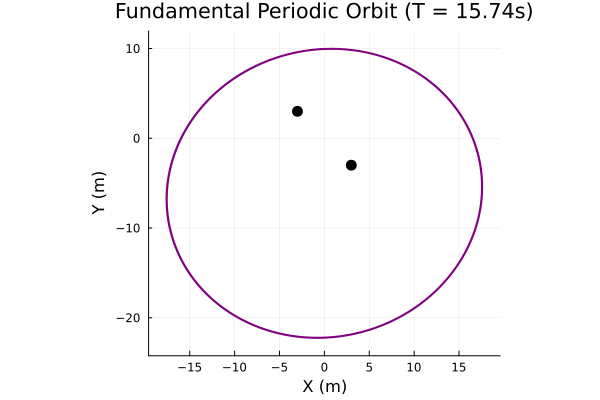
\includegraphics[width=\textwidth]{question13/periodic_orbit_static2.png}
        \caption{}
        \label{fig:top_left}
    \end{subfigure}
    \hfill % Pushes the subfigures apart
    \begin{subfigure}[b]{0.48\textwidth}
        \centering
        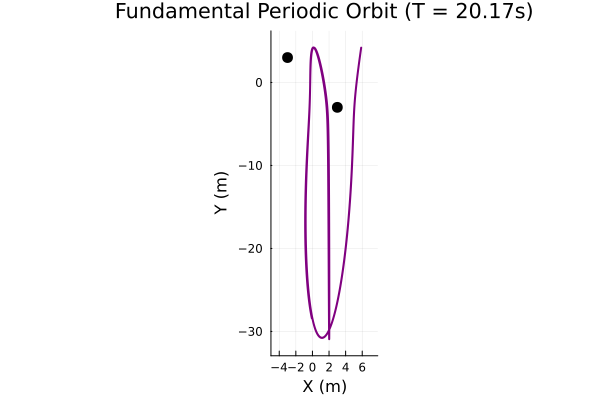
\includegraphics[width=\textwidth]{question13/periodic_orbit_static4.png}
        \caption{}
        \label{fig:top_right}
    \end{subfigure}

    \vspace{0.5cm} % Adds vertical space between the rows

    % --- Bottom Row ---
    \begin{subfigure}[b]{0.48\textwidth}
        \centering
        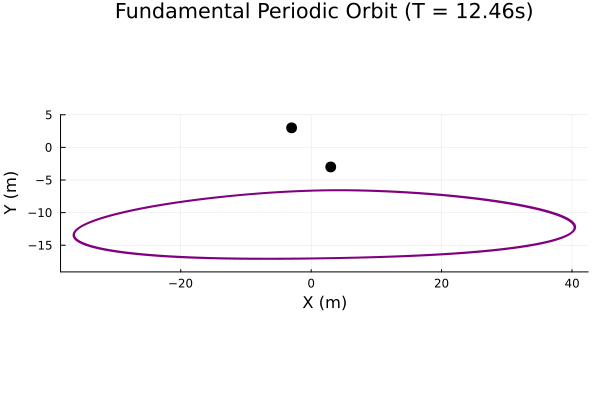
\includegraphics[width=\textwidth]{question13/periodic_orbit_static5.png}
        \caption{}
        \label{fig:bottom_left}
    \end{subfigure}
    \hfill
    \begin{subfigure}[b]{0.48\textwidth}
        \centering
        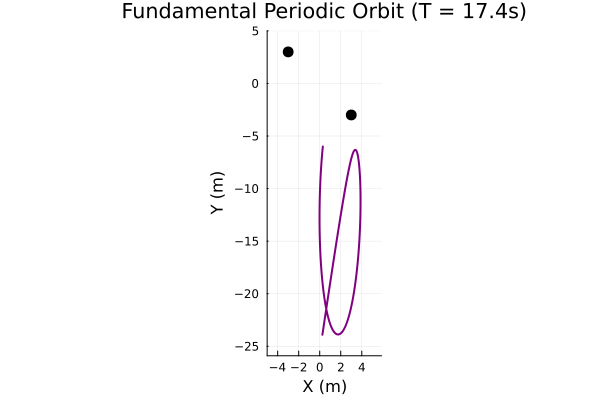
\includegraphics[width=\textwidth]{question13/periodic_orbit_static6.png}
        \caption{}
        \label{fig:bottom_right}
    \end{subfigure}

    \caption{Periodic solutions discovered from stricter tolerances ($10^{-11}$)}
    \label{fig:main_2x2_matrix}
\end{figure}

\begin{equation}
    G(u_0, T) = \Phi(u_0, T) - u_0 = 0
\end{equation}

However, for autonomous systems (where the rate of change of the system depends entirely on the state and not explicitly on time), translational invariance leads to an underdefined Shootiing Function. To combat this, a Poincare Map is used. The Poincare Map introduces a Constraint Plane $\Sigma$, asserting that the initial state $X_0$ must lie on $\Sigma$.


It is observed that the program finds significant fewer solutions when the tolerances of the fifth order solver used to solve for the sysem is lower ($10^{-8}$). The program is allowed to explore more solutions when the tolerances are reduced to the order of $10^{-11}$.

\vfill

\section{Systems with Periodic Motion}

\subsection{Neutrally Stable Periodic Motion}
Neutrally Stable Periodic Motion is the term given to periodic dynamics where perturbations to the system do not cause growth to infinity, nor does it cause the system to collapse to an attractor.\\

The best example of such a system is the \textbf{harmonic oscillator}. For a two-dimensional uncoupled system, the equations of motion are defined as:

\begin{equation}
    \begin{aligned}
        \ddot{x} &= -k_x x \\
        \ddot{y} &= -k_y y
    \end{aligned}
\end{equation}

\begin{figure}[h!]
    \centering
    \begin{subfigure}[b]{0.45\textwidth}
        \centering
        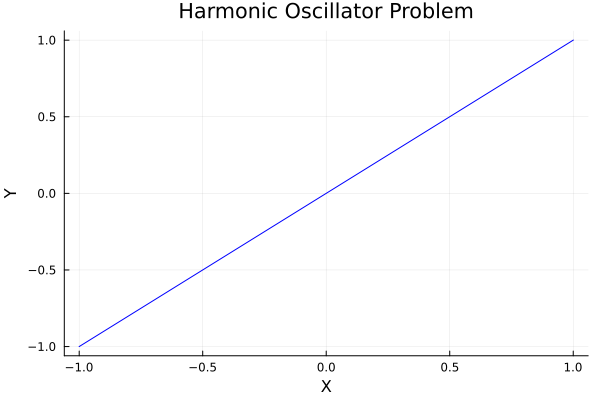
\includegraphics[width=\textwidth]{question14/harmonic.png}
        \caption{Unperturbed harmonic osicalltor}
    \end{subfigure}
    \hfill
    \begin{subfigure}[b]{0.45\textwidth}
        \centering
        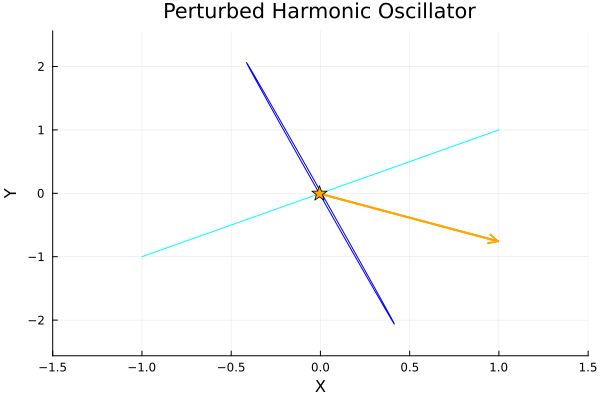
\includegraphics[width=\textwidth]{question14/perturbed_harmonic_oscillator.png}
        \caption{Perturbed harmonic osicallator}
    \end{subfigure}
    \caption{Phase portrait of a neutrally stable harmonic oscillator.}
    \label{fig:harmonic-oscillator}
\end{figure}

\subsection{Unstable Periodic Motion}
Unstable periodic motion occurs when a system possesses a periodic orbit, but any infinitesimal perturbation causes the trajectory to diverge violently from that orbit -- either escaping to infinity, collapsing into a stable fixed point, or transitioning into chaotic behavior (as is seen with the Lorenz Attractor).

\subsubsection{The Unstable Circular Repeller}
The Unstable Circular Repeller features a geometric circle as its unstable limit cycle. A particle starting exactly on the defined radius $R$ will orbit indefinitely, but any deviation will cause it to spiral inward to the origin or outward to infinity. The Cartesian state equations are

\begin{equation}
    \begin{aligned}
        \dot{x} &= y + x(x^2 + y^2 - R^2) \\
        \dot{y} &= -x + y(x^2 + y^2 - R^2)
    \end{aligned}
\end{equation}

\begin{figure}[h!]
    \centering
    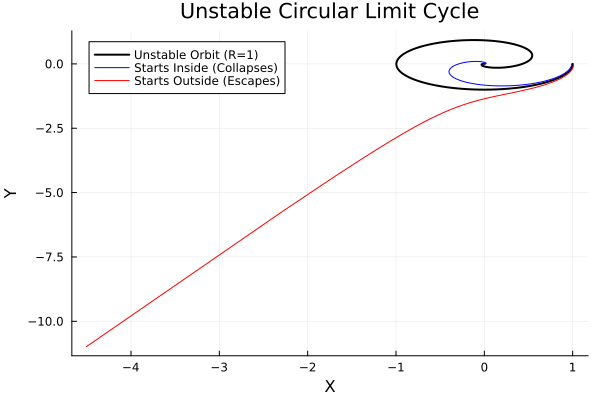
\includegraphics[width=0.6\textwidth]{question14/circular_repeller.png}
    \caption{Phase portrait demonstrating trajectories fleeing the unstable circular limit cycle.}
    \label{fig:circular-repeller}
\end{figure}

\subsubsection{The Reversed Van der Pol Oscillator}
Unlike the geometric repeller, the reversed Van der Pol oscillator represents a system with non-linear damping. By flipping the sign of the damping coefficient $\mu$ from the standard model, the traditional stable limit cycle becomes an unstable "ridge" in phase space. The governing second-order differential equation is

\begin{equation}
    \ddot{x} + \mu(1 - x^2)\dot{x} + x = 0
\end{equation}

\begin{figure}[h!]
    \centering
    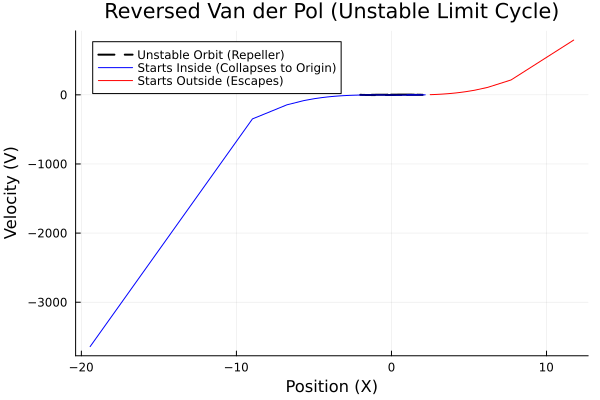
\includegraphics[width=0.6\textwidth]{question14/reverse_vdp.png}
    \caption{Phase space trajectories diverging from the reversed Van der Pol limit cycle.}
    \label{fig:reversed-vdp}
\end{figure}

\subsubsection{The Lorenz Attractor}
While the Lorenz system is globally bounded (trajectories do not escape to infinity), it exhibits extreme local instability within its strange attractor. Two infinitesimally close trajectories will exponentially diverge over time, demonstrating chaotic sensitive dependence on initial conditions. Visually this system does not exhibit obvious "unstable" behavior due to its chaotic nature. The system is defined by

\begin{equation}
    \begin{aligned}
        \dot{x} &= \sigma(y - x) \\
        \dot{y} &= x(\rho - z) - y \\
        \dot{z} &= xy - \beta z
    \end{aligned}
\end{equation}

\begin{figure}[h!]
    \centering
    \begin{subfigure}[b]{0.45\textwidth}
        \centering
        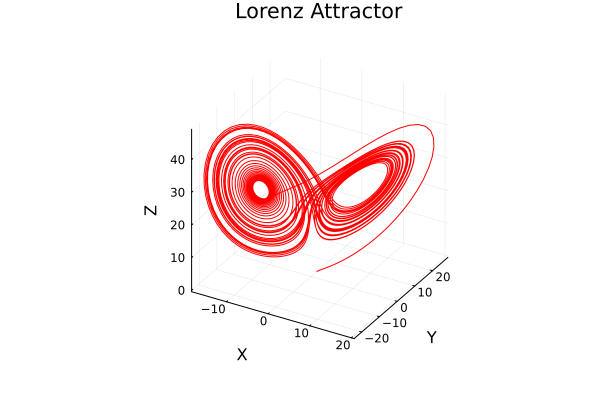
\includegraphics[width=\textwidth]{question14/loerentz.png}
        \caption{Standard Trajectory}
    \end{subfigure}
    \hfill
    \begin{subfigure}[b]{0.45\textwidth}
        \centering
        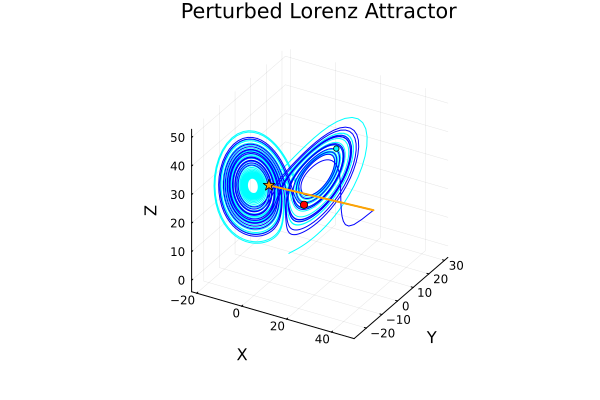
\includegraphics[width=\textwidth]{question14/perturbed_lorenz_final.png}
        \caption{Perturbed Trajectory ($\Delta = 10^{-5}$)}
    \end{subfigure}
    \caption{Chaotic divergence in the Lorenz attractor due to a microscopic initial perturbation.}
    \label{fig:lorenz-comparison}
\end{figure}

\subsection{Asymptotically Stable Periodic Motion}
Asymptotic stability in periodic systems is characterized by a \textbf{limit cycle}. This is a closed trajectory in phase space such that at least one other trajectory spirals into it as time approaches infinity. Unlike conservative systems, these are dissipative systems where energy is balanced non-linearly.

The most prominent example is the \textbf{Van der Pol Oscillator}. The system is governed by a second-order non-linear differential equation where the damping coefficient depends on the position $x$:

\begin{equation}
    \ddot{x} - \mu(1 - x^2)\dot{x} + x = 0
\end{equation}

In this system, $\mu$ represents the non-linearity and damping strength. For any initial condition $u_0 \neq (0,0)$, the trajectory eventually "locks" onto the limit cycle. This convergence is shown in Figure \ref{fig:vdp-stable}, where paths starting both inside and outside the cycle converge to the same steady-state periodic motion.



\begin{figure}[h!]
    \centering
    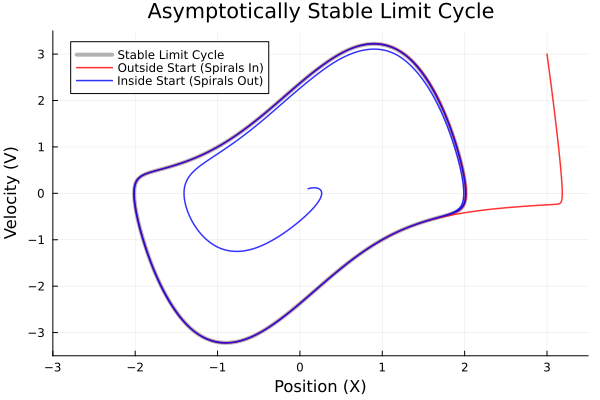
\includegraphics[width=0.7\textwidth]{question14/vdp.png}
    \caption{Phase portrait of the Van der Pol oscillator ($\mu = 1.5$). The red and blue trajectories represent transient states converging asymptotically to the black limit cycle.}
    \label{fig:vdp-stable}
\end{figure}


\section{Initial Value Problem with Collocation}

\subsection{Review: Euler's Method}

Given a system

\begin{equation}
    \ddot{x}(t) = -1 \qquad t \in 0, 1
\end{equation}

which is reduced to a coupled first order system

\begin{eqnarray}
    \ddot{x} = \dot{v} = -1 \nonumber \\
    v = \dot{x}.
\end{eqnarray}

The initial conditions are assumed to be $x(0) = 0$ and $v(0) = 0.5$.\\
\\
The Euler Integration Formula is utilized to solve for this system.

\begin{figure}[h!]
    \centering
    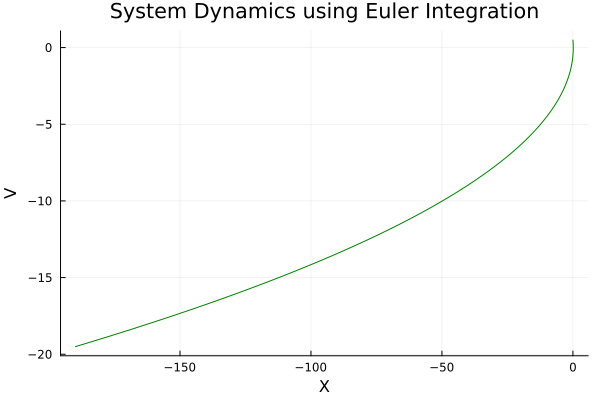
\includegraphics[width=0.6\textwidth]{question15/euler.png}
    \caption{Euler Integration Solution}
\end{figure}


\subsection{Trapezoidal Intgration}

It is hypothesised that one may improve the accuracy of the integrator should they use the trapezoidal integrator in place of Euler's integrator.

\begin{equation}
    z_{n+1} = z_n + h \frac{\dot{z}_n + \dot{z}_{n+1}}{2}
\end{equation}

\begin{minted}{julia}
function trapezoid_integration(u, time_step = 0.01)
    x, v = u
    dx, dv = system!(u)
    v_new = v + time_step * dv # Because dv is a constant here
    x_new = x + (time_step / 2.0) * (v + v_new)
    return x_new, v_new
end
\end{minted}

\begin{figure}[h!]
    \centering
    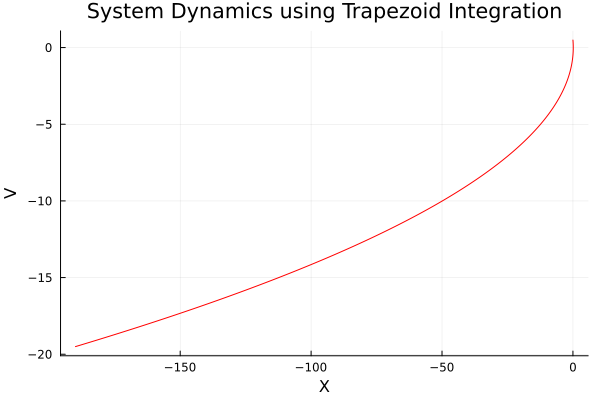
\includegraphics[width = 0.6\textwidth]{question15/trap_integration.png}
    \caption{Trapezoid Integration Solution}
\end{figure}

To confirm the earlier hypothesis, one may observe the error of the solutions against the analytic solution of the system.

\begin{eqnarray}
    v(t) = \int -1 \; dt = -t + v_0 = -t + 0.5 \nonumber \\
    x(t) = \int v \; dt = \int (0.5 - t) \; dt = 0.5t - 0.5t^2
\end{eqnarray}

\begin{figure}[h!]
    \centering
    \begin{subfigure}[b]{0.45\textwidth}
        \centering
        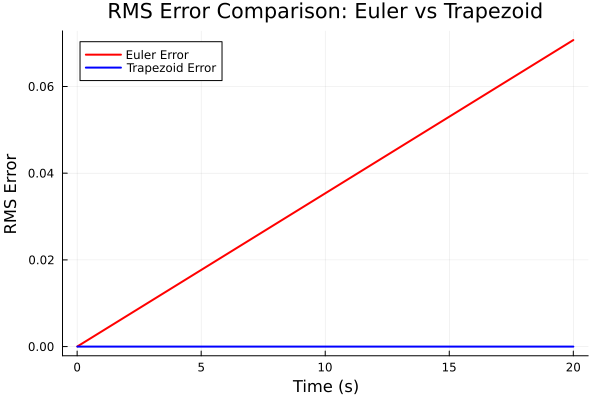
\includegraphics[width=\textwidth]{question15/error_comparison.png}
        \caption{Error Comparison}
    \end{subfigure}
    \hfill
    \begin{subfigure}[b]{0.45\textwidth}
        \centering
        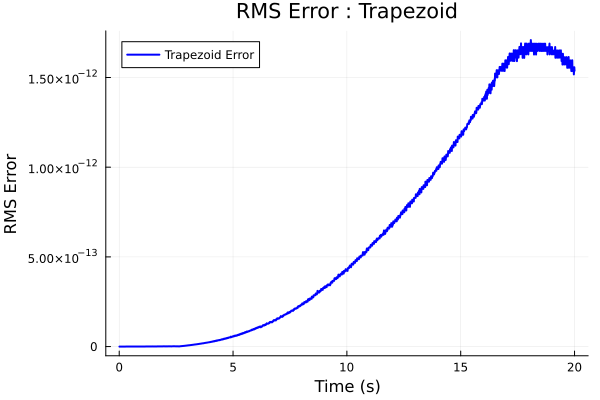
\includegraphics[width=\textwidth]{question15/trap_error.png}
        \caption{RMS Error : Trapezoidal Integration}
    \end{subfigure}
    \caption{Integration Errors}
    \label{fig:lorenz-comparison}
\end{figure}

It is abundantly clear that the trapezoidal integrator has significantly lesser error that its single-order counterpart.

\begin{figure}[h!]
    \centering
    \begin{subfigure}[b]{0.45\textwidth}
        \centering
        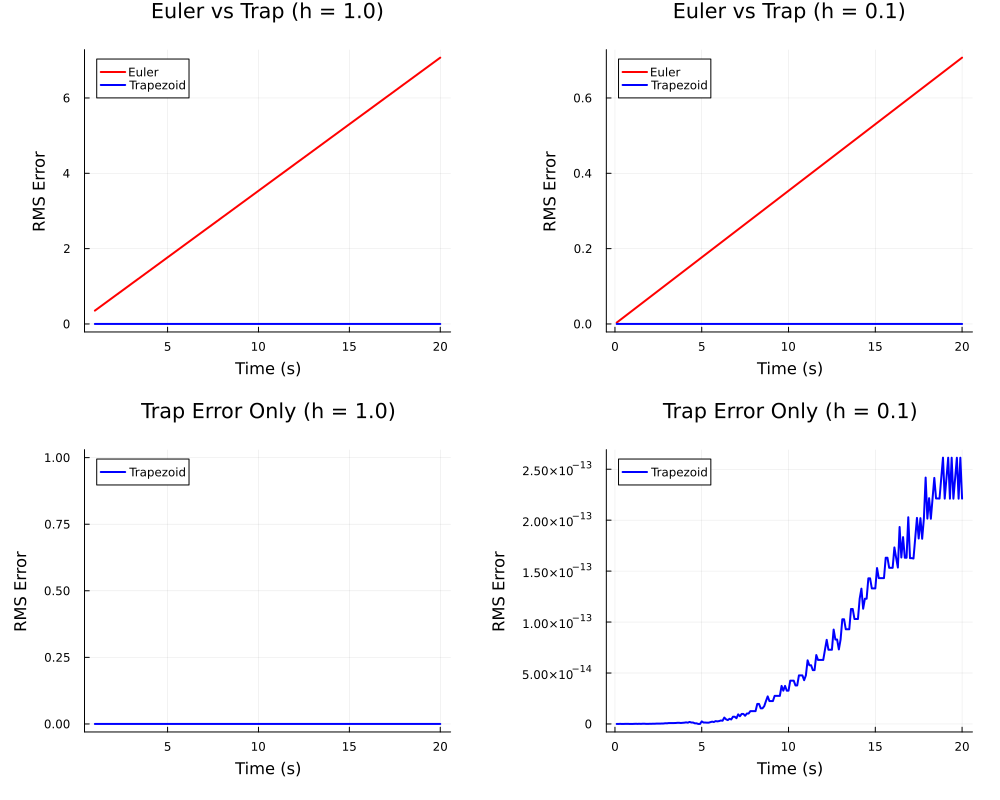
\includegraphics[width=\textwidth]{question15/error_with_h1.png}
    \end{subfigure}
    \hfill
    \begin{subfigure}[b]{0.45\textwidth}
        \centering
        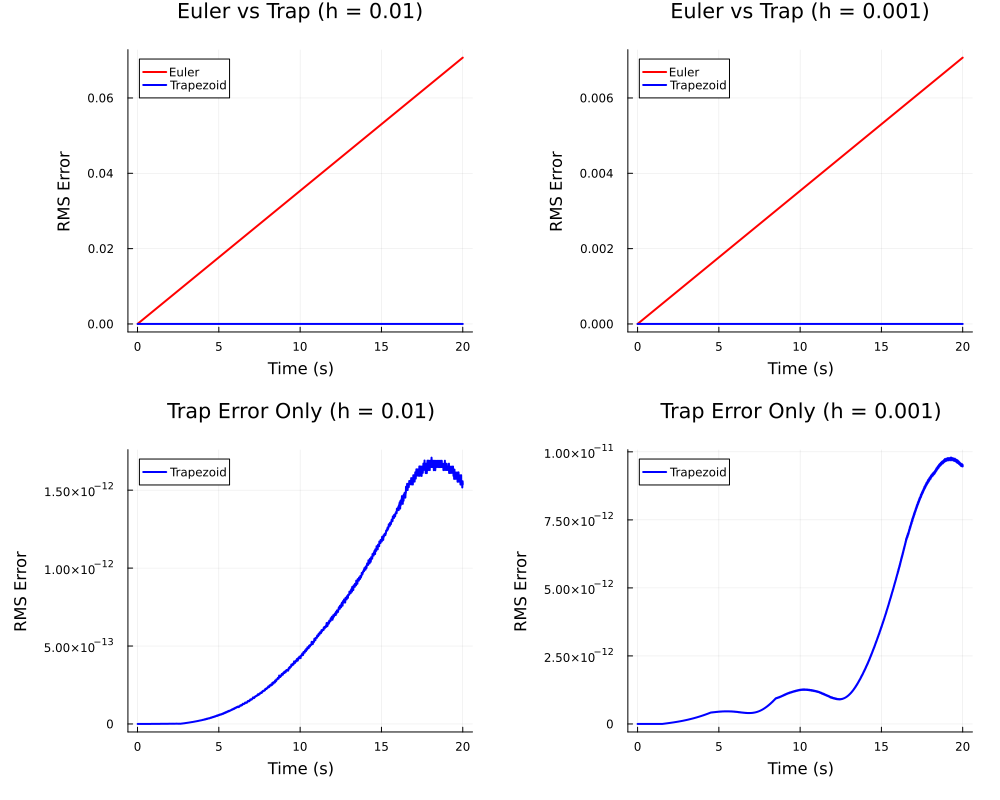
\includegraphics[width=\textwidth]{question15/error_with_h2.png}
    \end{subfigure}
    \caption{Integration Errors}
    \label{fig:lorenz-comparison}
\end{figure}

\section{Boundary Value Problems and The Shooting Method}

Consider a Boundary Value Problem

\begin{eqnarray}
    \ddot{x}(t) = -1 \nonumber \\
    x(0) = 0, \quad x(1) = 0. \\
\end{eqnarray}

In order to solve this problem, first one must define a shooting function $F$.

\begin{equation}
    F(s) = x(t = 1; s)
\end{equation}

for some value $s$. In other words, $x(1;s) = x(t = 1)$ given that $\dot{x}(0) = s$. To visualize this, one may plot a $F(s)$ vs $s$ graph.\\

\begin{figure}[!h]
    \centering
    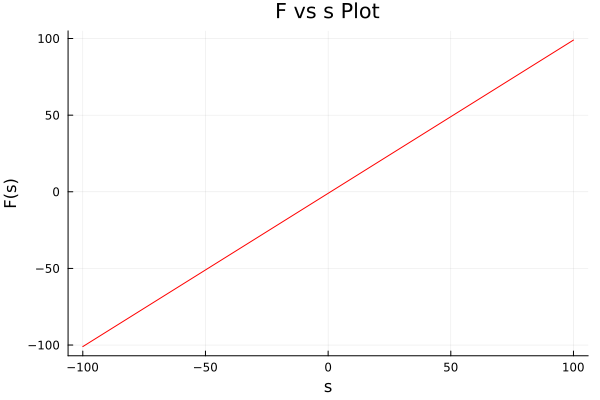
\includegraphics[width=0.5\textwidth]{question16/F_vs_s_plot.png}
    \caption{$F$ vs $s$ Plot}
\end{figure}

One may solve for the residual of the shooting function and required final value of $x$ using a numerical root-finding method to determine a suitable value for $s$. Here, the \textit{bisection method} is used. An example program in julia is given below.
\newpage

\begin{minted}{julia}
function bisection_solve(
    func,
    a,
    b,
    tol = 1e-5,
    max_iter = 1e+5
)
    fa = func(a)
    fb = func(b)

    # NOTE: f(a) and f(b) must have different signs in order for the method to work
    # Check for the above Conditions

    if (fa * fb > 0)
        return true  # Return true :: Error flag = 1
    end

    # Init midpoint
    c = a
    
    for i in 1:max_iter
        c = (a+b)/2
        fc = func(c)

        if (abs(fc) < tol) || ((b - a) / 2 < tol)
            return c
        end

        # Check for sign changes
        if (fa * fc < 0)
            # Discard right hand side
            fb = fc 
            b = c
        elseif (fb * fc < 0)
            # Discard left hand side
            fa = fc 
            a = c
        end
    end

    return c
end  
\end{minted}

The program returns a result of $v(0) = 0.500$. One may verify this result analytically.

\begin{figure}[h!]
    \centering
    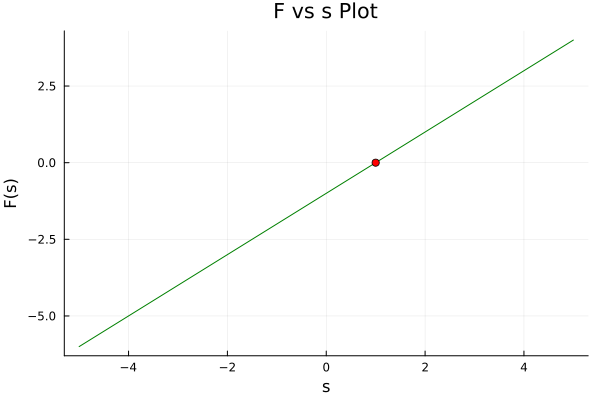
\includegraphics[width=0.3\textwidth]{question16/FS_solution.png}
    \caption{Numerical Solution}
\end{figure}

\section{Introduction to Collocation}

In this section, the discussion shifts from forward methods (like Euler Integration) and shooting methods to the concept of \textit{collocation}.

\subsection{The Theory}
A first-order system similar to the system used in the last two questions is used as an example. Between $t_0$ and $t_f$, some $N$ points are chosen uniformly spread apart, essentiially dividing the system into $N+1$ evenly spcaed intervals. A vector $z$ is used to hold all of the $x$ and $v$ values at each interval point.

\begin{equation}
    z = 
    \begin{bmatrix}
    x_1, x_2, x_3, \dots , v_1, v_2, v_3, \dots    
    \end{bmatrix}
\end{equation}

From the given boundary conditions, it is known that $x_1 = x_0$ and $x_{N+1} = x_f$. The remaining $N-2$ equations are written out to follow Euler's Method.

\begin{eqnarray}
    x_{k+1} = x_k + h \cdot v_k \nonumber \\
    v_{k+1} = v_k + h \cdot a \nonumber \\ \text{where } a = \ddot{x} \text{ is a constant.}
\end{eqnarray}

This part needs to be completed...

\subsection{Execution}
\begin{minted}{julia}
function collocation_solve(N, t_start = 0.0, t_end = 1.0)
    h = (t_end - t_start) / N
    num_points = N + 1

    # Extract system acceleration
    _, a = system!((0,0))

    # Total unknowns
    total_vars = 2 * num_points

    # Init matrices
    A = zeros(total_vars, total_vars)
    b = zeros(total_vars) # Collocation

    # x(1) = 0
    A[1,1] = 1.0
    b[1] = 0.0

    # x(N+1) = 0
    A[2, num_points] = 1.0
    b[2] = 0.0

    # -- Enforce Euler Discretization -- #
    row = 3 # 1 and 2 have been used up in the boundary Conditions
    for k in 1:N
        # -- Index Helpers -- #
        idx_xk = k
        idx_xnext = k + 1
        idx_vk = num_points + k
        idx_vnext = num_points + k + 1

        # -- Populate Matrices -- #
        # Rule: x_{k+1} - x_k - h*v_k = 0
        A[row, idx_xnext] = 1.0
        A[row, idx_xk] = -1.0
        A[row, idx_vk] = -h
        b[row] = 0.0
        row += 1
        # Rule: v_{k+1} - v_k = a*h
        A[row, idx_vnext] = 1.0
        A[row, idx_vk] = -1.0
        b[row] = a*h

        row += 1
    end
    # --- Solve for the Linear System Az = b ---- #
    z = A \ b
    # ---- Upack Solution ---- #
    x_sol = z[1:num_points]
    v_sol = z[num_points+1:end]
    time_array = range(t_start, t_end, length = num_points)

    return time_array, x_sol, v_sol
end
\end{minted}

\begin{figure}[htbp]
    \centering
    
    % --- Row 1 ---
    \begin{subfigure}{0.48\textwidth}
        \centering
        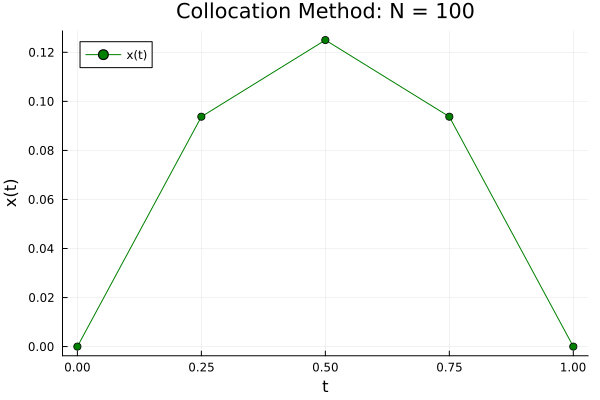
\includegraphics[width=\linewidth]{question17/collocationxt_4.png}
        \caption{}
        \label{fig:row1_left}
    \end{subfigure}
    \hfill
    \begin{subfigure}{0.48\textwidth}
        \centering
        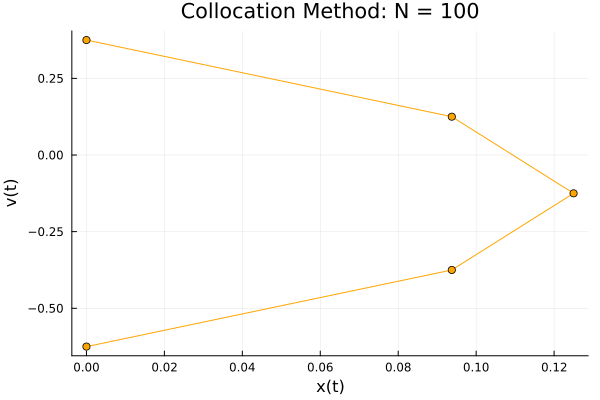
\includegraphics[width=\linewidth]{question17/collocation_4.png}
        \caption{}
        \label{fig:row1_right}
    \end{subfigure}

    \vspace{1em} % Space between rows

    % --- Row 2 ---
    \begin{subfigure}{0.48\textwidth}
        \centering
        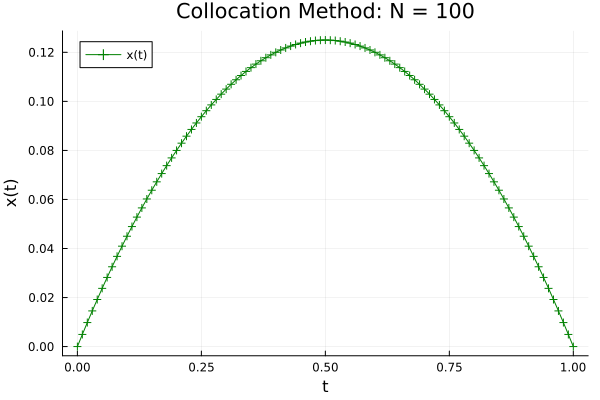
\includegraphics[width=\linewidth]{question17/collocationxt_100.png}
        \caption{}
        \label{fig:row2_left}
    \end{subfigure}
    \hfill
    \begin{subfigure}{0.48\textwidth}
        \centering
        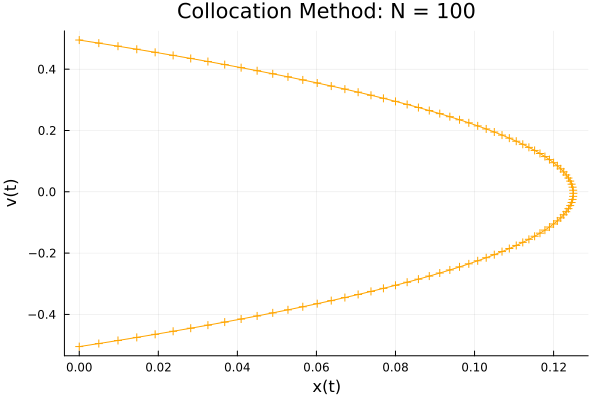
\includegraphics[width=\linewidth]{question17/collocation_100.png}
        \caption{}
        \label{fig:row2_right}
    \end{subfigure}

    \vspace{1em} % Space between rows

    % --- Row 3 ---
    \begin{subfigure}{0.48\textwidth}
        \centering
        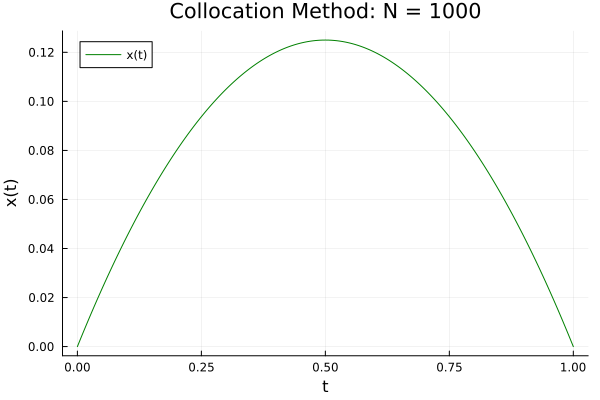
\includegraphics[width=\linewidth]{question17/collocationxt_1000.png}
        \caption{}
        \label{fig:row3_left}
    \end{subfigure}
    \hfill
    \begin{subfigure}{0.48\textwidth}
        \centering
        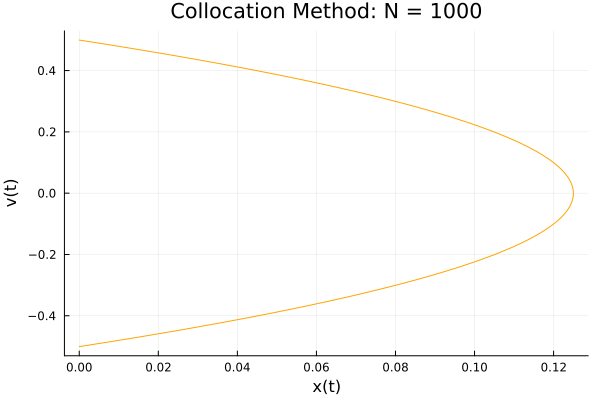
\includegraphics[width=\linewidth]{question17/collocation_1000.png}
        \caption{}
        \label{fig:row3_right}
    \end{subfigure}

    \caption{Collocation Results}
    \label{fig:six_panel_grid}
\end{figure}

\newpage 

\subsection{Comparing Results to the Shooting Method}

Both methods utilize the same Euler discretization. Any residual between the two methods should be driven primarily by the tolerance in the Bisection Method.

\begin{figure}[htbp]
    \centering
    % First Image (Left)
    \begin{subfigure}{0.48\textwidth}
        \centering
        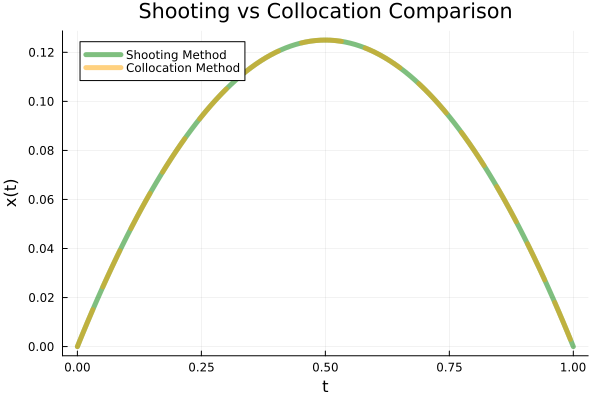
\includegraphics[width=\linewidth]{question17/compare_to_shooting.png}
        \caption{}
        \label{fig:left_image}
    \end{subfigure}
    \hfill % This is the magic that pushes them to the margins
    % Second Image (Right)
    \begin{subfigure}{0.48\textwidth}
        \centering
        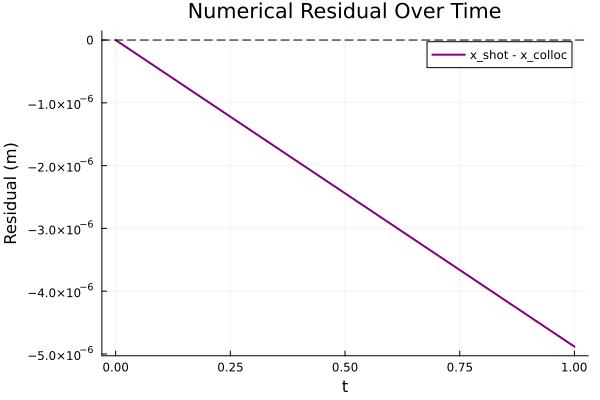
\includegraphics[width=\linewidth]{question17/compare_residual.png}
        \caption{}
        \label{fig:right_image}
    \end{subfigure}

    \caption{Comparing Collocation to the Shooting Method Results}
    \label{fig:side_by_side_comparison}
\end{figure}

The maximum residue observed here was $\delta = 4.88 \times 10^{-6}$ --- negligible. This is while the Bisection Method has \texttt{tol} = $10^{-5}$.

\section{Optimal Control : Euler Integration}

The objective of this problem is to find the optimal control force $u(t)$ that moves a unit mass ($m=1$) from rest at the origin to a target position at rest, while minimizing the total energy expended. The system dynamics are governed by the differential equations:
\begin{align}
    \dot{x}(t) &= v(t) \\
    \dot{v}(t) &= u(t)
\end{align}
with the boundary conditions defined as starting at rest ($x(0)=0, v(0)=0$) and ending at rest at the target position one second later ($x(1)=1, v(1)=0$).\\
\\
The continuous objective function to minimize the energy of the system that is directly propotionate to $J$ given as
\begin{equation}
    J = \int_{0}^{1} u(t)^2 \, dt .
\end{equation}

To solve this continuous Boundary Value Problem (BVP) numerically, it is converted into a discrete optimization problem using the collocation method. The time domain $t \in [0, 1]$ is divided into $N$ equal intervals of step size $h = 1/N$.

The integral objective function is approximated as a discrete sum:
\begin{equation}
    \min_{x, v, u} \sum_{k=1}^{N} h \cdot u_k^2
\end{equation}

The continuous system dynamics are enforced as algebraic constraints at every time step using forward Euler discretization. For $k = 1, 2, \dots, N$:
\begin{align}
    x_{k+1} - x_k - h \cdot v_k &= 0 \\
    v_{k+1} - v_k - h \cdot u_k &= 0
\end{align}

This formulation transforms the differential equations into a constrained quadratic programming problem. The system was implemented in Julia using the \texttt{JuMP.jl} modeling language and solved via the \texttt{Ipopt} interior-point optimizer, effectively mirroring the functionality of MATLAB's \texttt{fmincon}.

\begin{minted}{julia}
using JuMP
using Ipopt

function optimize_trajectory(
    N;
    method = :euler
)
    t_start, t_end = t_span
    h = (t_end - t_start) / N

    # Initialize the Optimization Model
    model = Model(Ipopt.Optimizer)
    set_silent(model) # Shush

    # Define unknowns
    @variables(model, begin
        x[1:N+1]
        v[1:N+1]
        u[1:N+1]
    end)

    # Define Objective
    @objective(
        model,
        Min,
        sum(u[k]^2 * h for k in 1:N+1) # Minimize Energy
    )

    # -- Enforce Constraints -- #

    # Boundary
    @constraint(model, x[1] == x_span[1])
    @constraint(model, x[N+1] == x_span[2])
    
    @constraint(model, v[1] == v_span[1])
    @constraint(model, v[N+1] == v_span[2])

    # Physics
    if method == :euler
        for k in 1:N
            @constraint(model, x[k+1] == x[k] + h * v[k])
            @constraint(model, v[k+1] == v[k] + h * u[k])
        end
    elseif method == :trapezoid
        for k in 1:N
            @constraint(model, x[k+1] == x[k] + h/2 * (v[k] + v[k+1]))
            @constraint(model, v[k+1] == v[k] + h/2 * (u[k] + u[k+1]))
        end
    else
        error("Unrecognized integration method. Use :euler or :trapezoid")
    end

    # Solver
    optimize!(model) # Yay

    time_array = range(t_span[1], t_span[2], length = N+1)

    return time_array, value.(x), value.(v), value.(u)
end
\end{minted}

Figure \ref{fig:optimal_euler} displays the resulting state trajectories $x(t)$ and $v(t)$ alongside the optimal control sequence $u(t)$ for $N=50$ intervals. 

\begin{figure}[h!]
    \centering
    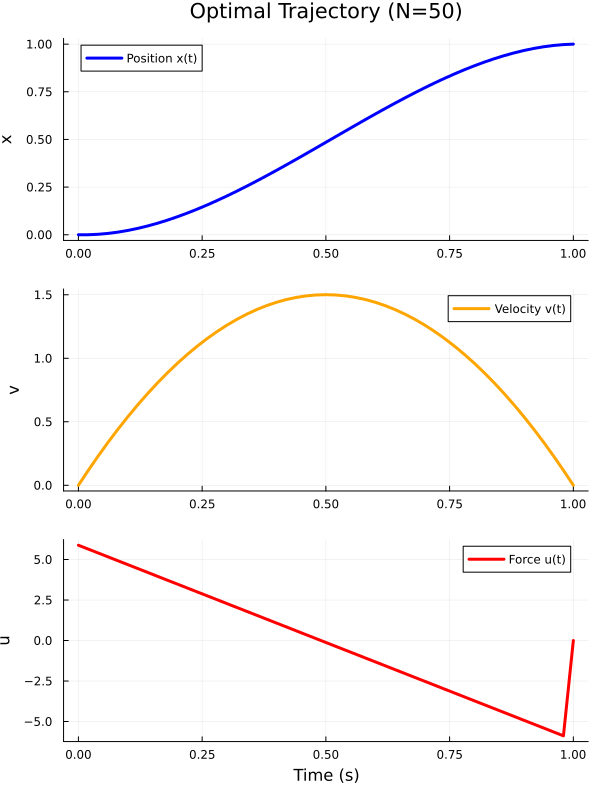
\includegraphics[width=0.5\textwidth]{question18/plot_euler.png}
    \caption{Optimal control trajectory using Euler discretization ($N=50$). Notice the slight asymmetry in the control force $u(t)$ resulting from the first-order temporal lag inherent to the Euler method.}
    \label{fig:optimal_euler}
\end{figure}

\section{Optimal Control : Trapezoid Integration}

In the previous section, an optimal control problem was solved using Euler Discretization. The same problem is solved using Trapezoidal Discretization in this section.

\begin{minted}{julia}
if method == :euler
        for k in 1:N
            @constraint(model, x[k+1] == x[k] + h * v[k])
            @constraint(model, v[k+1] == v[k] + h * u[k])
        end
    elseif method == :trapezoid
        for k in 1:N
            @constraint(model, x[k+1] == x[k] + h/2 * (v[k] + v[k+1]))
            @constraint(model, v[k+1] == v[k] + h/2 * (u[k] + u[k+1]))
        end
    else
        error("Unrecognized integration method. Use :euler or :trapezoid")
    end
\end{minted}

\begin{figure}[!h]
    \centering
    \begin{subfigure}{0.48\textwidth}
        \centering
        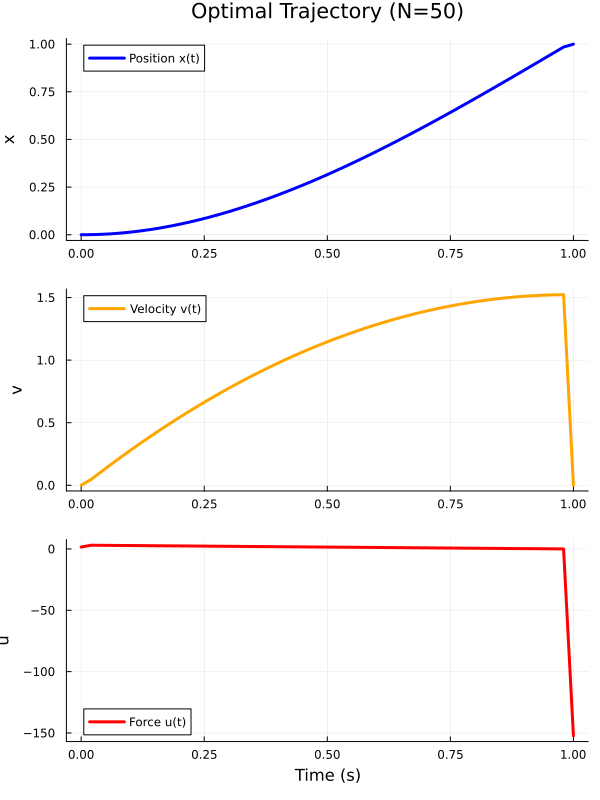
\includegraphics[width=\textwidth]{question18/plot_trapezoid.png}
    \end{subfigure}%
    \hfill
    \begin{subfigure}{0.48\textwidth}
        \centering
        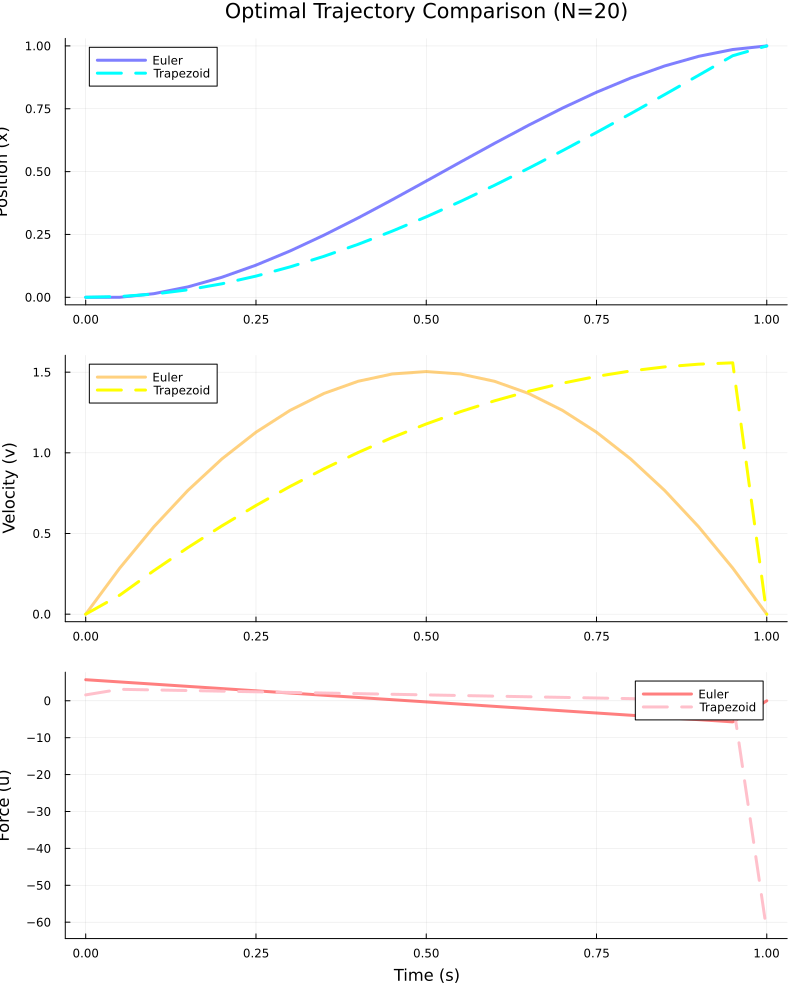
\includegraphics[width=\textwidth]{question18/compare.png}
    \end{subfigure}

    \caption{Trapezoidal Integration Collocation Results}
\end{figure}

It is evident that there are obvious differences between the trajectories optimized using Euler Discretization and Trapezoidal Discretization.

\section{Matrix Reconstruction and Numerical Jacobians}

\subsection{Reconstructing a Linear Black-Box (Matrix A)}
Suppose we have a black-box function that applies a linear transformation $u = A v$, where $A$ is an unknown $4 \times 4$ matrix:
\begin{equation}
    A = \begin{bmatrix}
    a_{11} & a_{12} & a_{13} & a_{14} \\
    a_{21} & a_{22} & a_{23} & a_{24} \\
    a_{31} & a_{32} & a_{33} & a_{34} \\
    a_{41} & a_{42} & a_{43} & a_{44}
    \end{bmatrix}
\end{equation}

To determine the individual elements of $A$ without analytical access, we systematically evaluate the function using the standard basis vectors. For example, multiplying $A$ by the first basis vector $e_1 = [1, 0, 0, 0]^T$ isolates the first column:
\begin{equation}
    A e_1 = \begin{bmatrix}
    a_{11} & a_{12} & a_{13} & a_{14} \\
    a_{21} & a_{22} & a_{23} & a_{24} \\
    a_{31} & a_{32} & a_{33} & a_{34} \\
    a_{41} & a_{42} & a_{43} & a_{44}
    \end{bmatrix}
    \begin{bmatrix} 1 \\ 0 \\ 0 \\ 0 \end{bmatrix}
    = \begin{bmatrix} a_{11} \\ a_{21} \\ a_{31} \\ a_{41} \end{bmatrix}
\end{equation}

By probing the system iteratively with $e_2, e_3,$ and $e_4$, we extract the remaining columns. The complete matrix is reconstructed by horizontally concatenating the resulting vectors. This is mathematically equivalent to passing the identity matrix $I_4$ through the system:
\begin{equation}
    A = \Big[ f(e_1) \;\Big|\; f(e_2) \;\Big|\; f(e_3) \;\Big|\; f(e_4) \Big] = A I_4
\end{equation}

\subsection{The Non-Linear Case (Numerical Jacobian)}
For non-linear systems, such as a full ODE simulation mapping an initial state $x_0$ to a final state $f(x_0)$, no global matrix $A$ exists. Instead, we seek the local linear approximation: the Jacobian matrix $J$.\\
\\
We construct $J$ column-by-column using a forward finite-difference approximation. We apply a small scalar perturbation $\epsilon$ in the direction of each standard basis vector $e_j$. The change in the system's output relative to the nominal unperturbed trajectory isolates the rate of change with respect to that specific state variable:
\begin{equation}
    \Delta y = f(x_0 + \epsilon e_j) - f(x_0)
\end{equation}
Dividing by the step size yields the $j$-th column of the Jacobian:
\begin{equation}
    J_{*, j} \approx \frac{f(x_0 + \epsilon e_j) - f(x_0)}{\epsilon}
\end{equation}

To build the full $n \times n$ Jacobian matrix, this finite-difference probing is repeated for all state variables. The resulting matrix $J$ can then be analyzed for its eigenvalues to determine the local stability of the system.

\section{Optimal Planning and Control}

\textbf{Problem Setup}
Consider a 2D point-mass model representing a drone or lander governed by the following equations of motion:
\begin{align}
    \dot{x} &= v_x \\
    \dot{z} &= v_z \\
    \dot{v}_x &= u_x \\
    \dot{v}_z &= u_z - g
\end{align}
where $g = 1.62 \text{ m/s}^2$ represents the gravitational acceleration (e.g., lunar gravity).

\textbf{Boundary Conditions}
The system is subject to the following initial conditions at $t = 0$:
\begin{equation}
    x(0) = x_0, \quad z(0) = z_0, \quad v_x(0) = v_{x0}, \quad v_z(0) = v_{z0}
\end{equation}
The target final conditions at an unspecified or specified terminal time $T$ require a precise landing at the origin with zero velocity:
\begin{equation}
    x(T) = 0, \quad z(T) = 0, \quad v_x(T) = 0, \quad v_z(T) = 0
\end{equation}

\textbf{Constraints}
\begin{itemize}
    \item \textbf{Control Constraint:} The total thrust magnitude is bounded by a maximum capability $u_{\max}$:
    \begin{equation}
        \sqrt{u_x^2 + u_z^2} \le u_{\max}
    \end{equation}
    \item \textbf{State Constraint:} The vehicle must remain above or at ground level throughout the trajectory:
    \begin{equation}
        z \ge 0
    \end{equation}
\end{itemize}

\subsection{Optimal Plan}
With the objective of minimizing the control effort

\begin{equation}
    \min \int_0^T ||u(t)||^2 dt
\end{equation}

this can be posed as an optimization problem. The system is given the initial state $(x, z, v_x, v_z) = (5, 10, -1, -2)$ and solved using collocation.

\begin{figure}
    \centering
    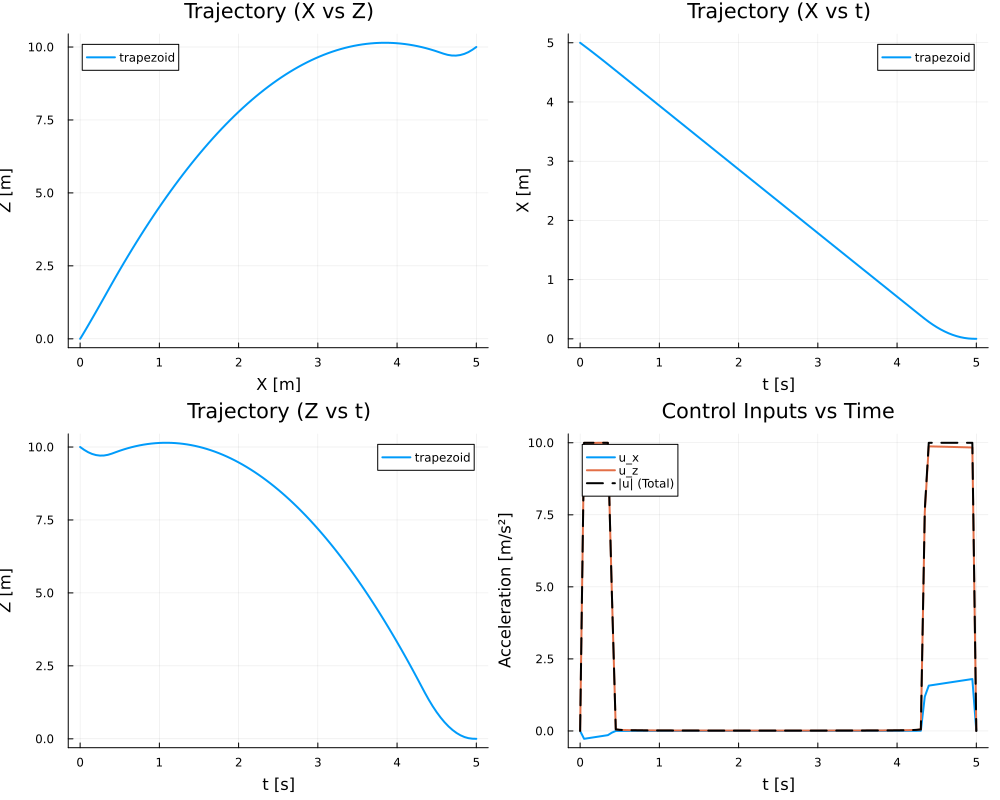
\includegraphics[width=0.7\textwidth]{question21/all.png}
    \caption{Trajectory and Control of the Ideal System}
\end{figure}

\subsection{Controllable Region Estimation}
This subsection focuses on estimating a controllable region. This section is unnecessarily overcomplicated.

\subsubsection{Monte Carlo Sampling}
The first approach considered was an Monte Carlo approach. With fixed initial velocities, the $x$--$z$ space is sampled using a uniform distribution. The system run through the non-linear optimizer. Chosen points are classified into ``Feasible'' and ``Infeasible'' classes depending on whether or not the optimizer could solve the problem locally or not.

\begin{minted}{julia}
# ---- Monte Carlo Engine ---- #
function MC(num_samples, x_bounds, z_bounds)
    x_dist = Uniform(x_bounds[1], x_bounds[2])
    z_dist = Uniform(z_bounds[1], z_bounds[2])

    # Store raw MC data
    mc_x = Float64[]
    mc_z = Float64[]
    mc_status = Float64[] # 1.0 for feasible, 0.0 for infeasible

    for i in 1:num_samples
        sample_x = rand(x_dist)
        sample_z = rand(z_dist)
        
        state_zero = (sample_x, sample_z, -1.0, -2.0)
        state_end = (0.0, 0.0, 0.0, 0.0)

        # Using N=80 for slightly faster MC iterations
        is_feasible = optimize_trajectory(80, state_zero, state_end, (0.0, 5.0), 15.0, :trapezoid)

        push!(mc_x, sample_x)
        push!(mc_z, sample_z)
        push!(mc_status, is_feasible ? 1.0 : 0.0)
        
        if i % 50 == 0
            println("Completed $i / $num_samples samples...")
        end
    end

    println("Finished sampling! Interpolating data for contour plot...")
    return mc_x, mc_z, mc_status
end
\end{minted}

\begin{figure}[h!]
    \centering
    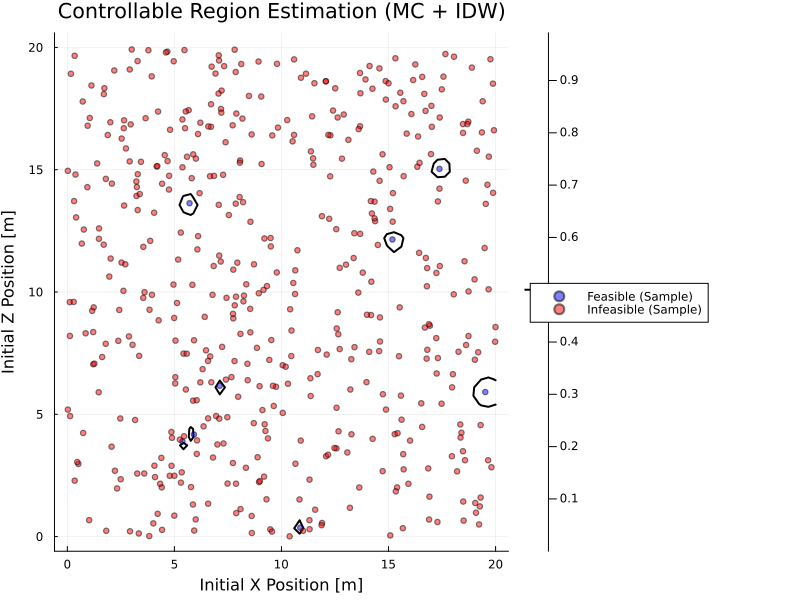
\includegraphics[width=0.5\textwidth]{question21/MC_contours.png}
    \caption{MC Convergence Contours}
\end{figure}

This approach was time consuming, and the results make it fairly clear that this was an unwise approach.

\subsubsection{Random Walks}
The next approach considered was Random Walks. The system was initialized at the final state of the problem and allowed to carry out a random walk -- the direction of the control was chosen randomly and the maximum available magnitude of control was applied. This method is much cheaper computationally, allowing a total of $10^8$ data points. Unfortunately, this method yields a probability distribution around the inital point, instead of the maximum reach. In hindsight, this too was an unwise approach.

\begin{minted}{julia}
function backward_random_reachability(num_samples, T, N, u_max)
    h = T / N
    
    valid_x0 = Float64[]
    valid_z0 = Float64[]
    valid_vx0 = Float64[]
    valid_vz0 = Float64[]

    println("Starting Backward Reachability Sampling ($num_samples trajectories)...")

    for i in 1:num_samples
        x, z = 0.0, 0.0
        vx, vz = 0.0, 0.0
        
        # Initialize random controls at the end-state
        theta = rand(Uniform(0, 2*pi))
        r = u_max * sqrt(rand()) 
        ux = r * cos(theta)
        uz = r * sin(theta)

        valid_trajectory = true

        for k in 1:N
            # Random Walk Controls
            ux += rand(Normal(0.0, 1.5))
            uz += rand(Normal(0.0, 1.5))
            
            # Clamp thrust vector magnitude to u_max
            mag = sqrt(ux^2 + uz^2)
            if mag > u_max
                ux = (ux / mag) * u_max
                uz = (uz / mag) * u_max
            end

            # Reverse Euler Integration
            vx_prev = vx - h * ux
            vz_prev = vz - h * (uz - g)
            
            x_prev = x - h * vx_prev
            z_prev = z - h * vz_prev

            # Update state for the next backward step
            x, z = x_prev, z_prev
            vx, vz = vx_prev, vz_prev

            if z < 0.0
                valid_trajectory = false
                break
            end
        end

        if valid_trajectory
            push!(valid_x0, x)
            push!(valid_z0, z)
            push!(valid_vx0, vx)
            push!(valid_vz0, vz)
        end
    end
\end{minted}

However, the idea that the system can be evolved backwards to see where it can start from and end up in the desired end-point can be pursued with smarter methods.

\begin{figure}[h!]
    \centering
    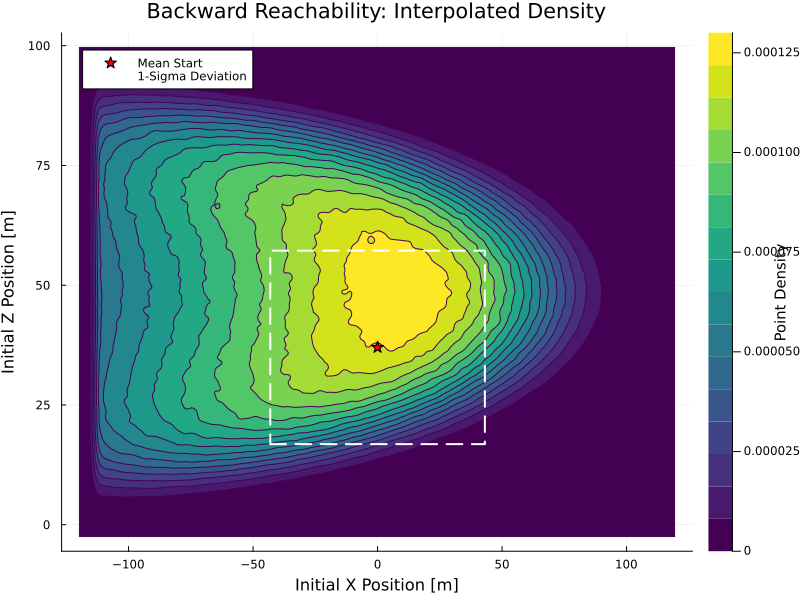
\includegraphics[width=0.5\textwidth]{question21/controled_randomwalk.png}
    \caption{Random-Walk Finishing Point Contours}
\end{figure}

\subsubsection{Maximum Reverse}
Instead of allowing the point to carry out a random walk, the point is assigned an angle at the start; control is applied at maximum magnitude in this direction for the entire duration of the simulation. This, very simply yields the maximum reach of control.

\begin{minted}{julia}
# ---- Deterministic Boundary Mapping ---- #
function map_reachability_boundary(
    num_angles, 
    T, 
    N, 
    u_max
)
    h = T / N
    
    # Arrays to store the discovered t=0 boundary states
    boundary_x0 = Float64[]
    boundary_z0 = Float64[]

    println("Starting Deterministic Boundary Sweep ($num_angles angles)...")

    # Sweep theta from 0 to 2π
    angles = range(0, 2*pi, length=num_angles)

    for (i, theta) in enumerate(angles)
        # Start at the target origin at T_final
        x, z, vx, vz = 0.0, 0.0, 0.0, 0.0
        
        valid_trajectory = true

        # Lock the max control effort in the current direction theta
        ux = u_max * cos(theta)
        uz = u_max * sin(theta)

        # Step backward in time
        for k in 1:N
            # Reverse Euler Integration
            vx_prev = vx - h * ux
            vz_prev = vz - h * (uz - g)
            
            x_prev = x - h * vx_prev
            z_prev = z - h * vz_prev

            # Update state for the next backward step
            x = x_prev
            z = z_prev
            vx = vx_prev
            vz = vz_prev

            # State constraint: Check if trajectory goes underground
            if z < 0.0
                valid_trajectory = false
                break
            end
        end

        # Only save the start points that never violate the ground constraint
        if valid_trajectory
            push!(boundary_x0, x)
            push!(boundary_z0, z)
        end
        
        if i % 100 == 0
            println("Swept $i / $num_angles directions...")
        end
    end

    println("Finished! Mapped $(length(boundary_x0)) boundary points.")
    return boundary_x0, boundary_z0
end 
\end{minted}

\begin{figure}[h!]
    \centering
    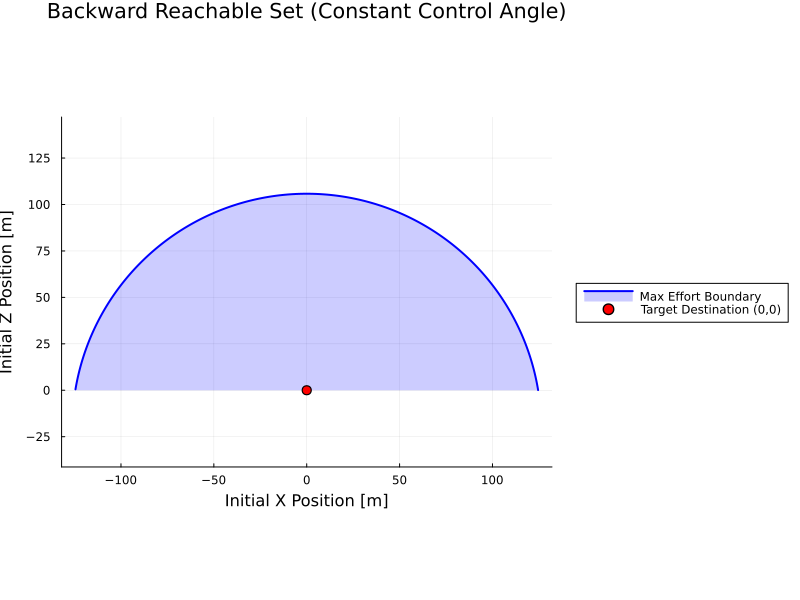
\includegraphics[width=0.5\textwidth]{question21/max_reach_contour.png}
\end{figure}

\section{Optimal Control with Perturbations}

In this section, it is demonstrated that path planning with optimal control is not useful in real-world applications where disturbances are introduced to the control. This section focuses on the same problem as the last section.

\begin{equation}
    u_\text{true} = \alpha u_\text{ideal}
\end{equation}

A disturbance is introduced to $u$ by introducing a term $\alpha$. An open-loop trajectory optimizer does not take this into account; and thus the planner fails.\\
\\
The optimizer is run as it is in the previous question, and the controls for each step are frozen. The disturbances are introduced to the system and the dynamics of the system are rerun from the initial state with these frozen weights. Here $\alpha \in [0.70, 0.90]$ .

\begin{minted}{julia}
for k in 1:N
    # Apply runtime disturbance
    α = rand() * (0.9 - 0.7) + 0.7
    
    # Step physics forward using frozen controls
    x_dist[k+1] = x_dist[k] + h * vx_dist[k]
    z_dist[k+1] = z_dist[k] + h * vz_dist[k]

    # Evolve with the frozen "nominal" controls
    vx_dist[k+1] = vx_dist[k] + h * ux_nom[k] * α
    vz_dist[k+1] = vz_dist[k] + h * (uz_nom[k] * α - g)
    
    # Calculate spatial error at the new step
    dx = abs(x_dist[k+1] - x_nom[k+1])
    dz = abs(z_dist[k+1] - z_nom[k+1])
    
    step_distance_error[k+1] = sqrt(dx^2 + dz^2)
    cumulative_difference[k+1] = cumulative_difference[k] + step_distance_error[k+1]
end
\end{minted}

As expected, the control fails. 

\begin{figure}[h!]
    \centering
    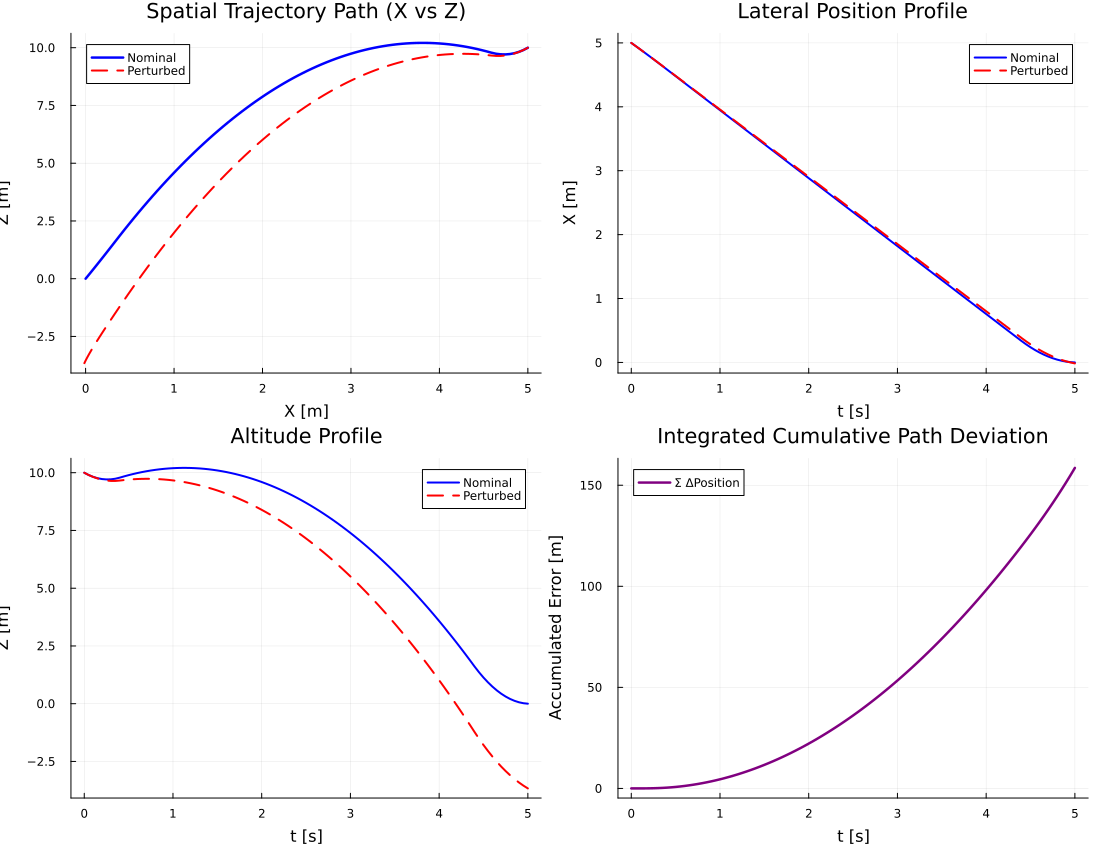
\includegraphics[width=0.6\textwidth]{question22/failure.png}
    \caption{Failure of open-loop control}
\end{figure}

\section{Model Predictive Control}

In order to introduce real-time control to a trajectory optimizer, one must update the controls with every step, taking into account the disturbance in the present and previous states.\\
\\
This is executed by first computing the ideal trajectory without any disturbance. Next, the real-time controller is given a cost function that punishes the system for deviating from the ideal trajectory. Conventionally, larger residuals in position are deemed costlier than residuals in velocity.\\
\\

The real-time controller is thus allowed to look $N_p$ steps into the future, allowing it to take into account future steps for its present control. The value $N_p$ is called the horizon distance.

The real-time cost function is given as

\begin{equation}
    \min \sum_{i=0}^{Np} 
    \Big(X - X_\text{ref}\Big)^T Q \Big(X - X_\text{ref}\Big)
    u^T R u
\end{equation}

where the matrices $Q$ and $R$ are used to assign cost weights to the positions and velocities, and the control effort respectively. Generally, $Q$ and $R$ are disgonal matrices. In this script, these matrices are diagonal and decomposed into a series of simple algebraic terms.

\begin{minted}{julia}
@objective(model, Min,
        sum(
            q[1] * (x[k]  - state_ref_horizon[k][1])^2 +
            q[2] * (z[k]  - state_ref_horizon[k][2])^2 +
            q[3] * (vx[k] - state_ref_horizon[k][3])^2 +
            q[4] * (vz[k] - state_ref_horizon[k][4])^2 +
            r[1] * ux[k]^2 +
            r[2] * uz[k]^2
            for k in 1:Np+1
        )
    )
\end{minted}

In this run, the disturbance $\alpha \sim \mathcal{N}(0.8, 0.33)$ is sampled from a normal distribution, and clamped between 0 and 1, \texttt{α = clamp(α, 0.0, 1.0)}.

\begin{minted}{julia}
function simulate_mpc_run(Np, n_steps, state_initial, ref_trajectory, Q, R, step_t, u_max, g, μ, σ)
    println("Running MPC Simulation for Np = $Np...")
    state_actual = copy(state_initial)
    trajectory_mpc = [copy(state_actual)]
    
    for t in 1:n_steps
        reference_start = t
        reference_end = min(t + Np, n_steps + 1)
        
        # Slice the dynamically feasible path
        state_ref_horizon = ref_trajectory[reference_start:reference_end]

        # Pad with the final target state
        while length(state_ref_horizon) < Np + 1
            push!(state_ref_horizon, ref_trajectory[end])
        end

        # Calculate optimal control
        ux_opt, uz_opt = solve_mcp(state_actual, state_ref_horizon, Q, R, Np, step_t, u_max)

        # Inject the Gaussian disturbance
        α = μ + σ * randn()
        α = clamp(α, 0.0, 1.0) # Keep efficiency strictly between

        u_applied = [α * ux_opt, α * uz_opt]

        # Step the true physics forward with the degraded control
        state_actual = step_dynamics(state_actual, u_applied, step_t, g)
        push!(trajectory_mpc, copy(state_actual))

        # Check for crashes
        if state_actual[2] <= 0.0
            break
        end
    end
    
    return trajectory_mpc
end
\end{minted}

\begin{figure}[h!]
    \centering
    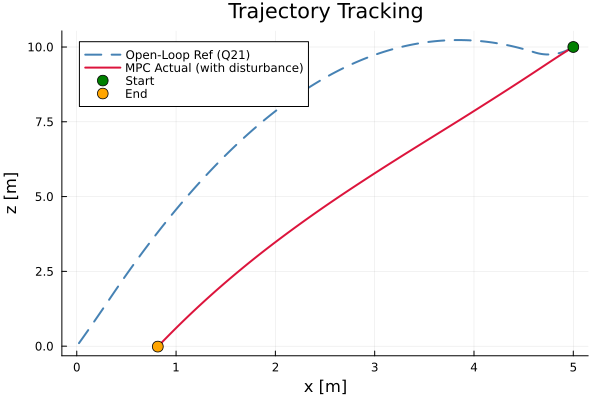
\includegraphics[width=0.6\textwidth]{question23/mpc.png}
    \caption{MPC, $N_p$ = 5}
\end{figure}

\subsection{Results of Varying the Horizon Distance}

Varying the horizon distance allows the optimizer to plan further ahead into the future. It is intuitively and experimentally evident that larger values of $N_p$ yield better results from the predictive controller.

\begin{figure}[h!]
    \centering
    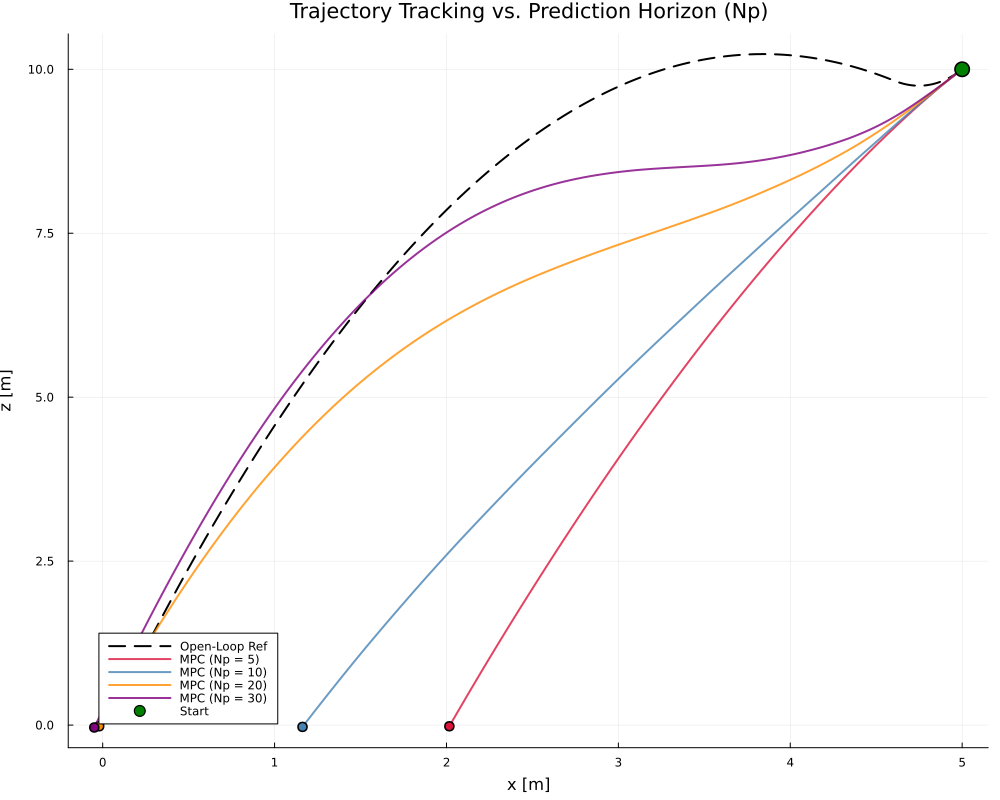
\includegraphics[width=0.6\textwidth]{question23/varying_NP.png}
    \caption{Results from varying $N_p$}
\end{figure}


\end{document}
